%Written by: The Smart Eraser Senior Design team!
%Project Manager: Heather Libecki
%Team Members: Chris Quesada and Juan Colin
%Let's get started!

\RequirePackage{filecontents}
\begin{filecontents*}{reference.bib}
	@misc{de1,
	author			={Altera},
	title			={{DE1\_SoC Reference Manual}},
	note			=	{\url{http://www.ee.ic.ac.uk/pcheung/teaching/ee2digital/DE1SoCUsermanual.pdf},
	}
}
	@misc{SM,
	author			={Oyostepper},
	title			={{23Hs22-2804S data sheet}},
	note			=	{\url{https://www.oyostepper.com/images/upload/File/23HS22-2804S.pdf},
	}
}
	@misc{SMD,
	author			={Leadshine Technology CO, Ltd},
	title			={{DM542 User Manual}},
	note			=	{\url{http://robokits.download/datasheets/Leadshine\%20DM542.pdf},
	}
}
	@misc{wifiStandards,
	author			={IEEE Standards Association},
	title			={{IEEE 802.15.3e-2017 - IEEE Standard for 
					High Data Rate Wireless Multi-Media Networks--Amendment 1: High-Rate Close Proximity Point-to-Point Communications}},
	note			=	{\url{https://standards.ieee.org/standard/802\_15\_3e-2017.html}
	}
}
	@misc{armStandards,
	author			={ARM Limited},
	title			={{Procedure Call Standard for the 
					ARM Architecture}},
	note			=	{\url{http://infocenter.arm.com/help/topic/com.arm.doc.ihi0042f/IHI0042F\_aapcs.pdf}
	}
}
	@misc{ieee,
	author			={IEEE},
	title			={{IEEE Editorial Style Manual }},
	note			=	{\url{https://www.ieee.org/content/dam/ieee-org/ieee/web/org/conferences/style\_references\_manual.pdf}
	}
}
	@misc{nema1,
	author			={National Electrical Manufacturers Association},
	title			={{NEMA Standards Publication ICS 16
					Motion/Position Control Motors,
					Controls, and Feedback Devices}},
	note			=	{\url{https://www.nema.org/Standards/SecureDocuments/ICS16.pdf}
	}
}
	@misc{nema2,
	author			={National Electrical Manufacturers Association},
	title			={{Occupancy Motion Sensors Standard}},
	note			=	{\url{https://www.nema.org/Standards/Pages/Occupancy-Motion-Sensors-Standard.aspx\#download}
	}
}
	@misc{cam,
	author			={sv3c},
	title			={{WiFi Camera Outdoor, SV3C 
				Surveillance CCTV, 1080P HD Night 
				Vision Bullet Cameras, Waterproof 
				Security Camera, IR LED Motion Detection 
				IP Cameras for Indoor Outdoor, Support Max 
				128GB SD Card }},
	note			=	{\url{https://www.amazon.com/dp/B07789DM4R/?coliid=I1G2VVNW6NF88L\&colid=22YAOKWOJAKA9\&psc=0\&ref\_=lv\_ov\_lig\_dp\_it}
	}
}
	@misc{raspB,
	author			={Raspberry Foundation},
	title			={{Products Page }},
	note			=	{\url{https://www.raspberrypi.org/products/raspberry-pi-3-model-b/}
	}
}
	@misc{smR,
	author			={STEPPERONLINE},
	title			={{Nema 23 CNC Stepper Motor 
					2.8A 178.5oz.in/1.26Nm CNC Stepping Motor DIY CNC Mill}},
	note			=	{\url{https://www.amazon.com/dp/B00PNEPF5I/?coliid=I3APKEM9Y17HEP\&colid=22YAOKWOJAKA9\&psc=0\&ref\_=lv\_ov\_lig\_dp\_it}
	}
}
	@misc{smdataR,
	author			={STEPPERONLINE},
	title			={{Stepper Motor}},
	note			=	{\url{https://www.omc-stepperonline.com/download/23HS22-2804S.pdf}
	}
}
	@misc{smdataD,
	author			={STEPPERONLINE},
	title			={{STEPPERONLINE CNC Stepper Motor Driver 1.0-4.2A 20-50VDC 1/128 Micro-step 
					Resolutions for Nema 17 and 23 Stepper Motor }},
	note			=	{\url{https://www.amazon.com/dp/B06Y5VPSFN/?coliid=I1R941FDJ72L0R\&colid=22YAOKWOJAKA9\&psc=0\&ref\_=lv\_ov\_lig\_dp\_it}
	}
}
	@misc{smdataDD,
	author			={STEPPERONLINE},
	title			={{User's Manual for DM542T}},
	note			=	{\url{https://www.omc-stepperonline.com/download/DM542T.pdf}
	}
}
	@misc{kuman,
	author			={Kuman},
	title			={{kuman 3 pcs nRF24L01+PA+LNA Antenna Wireless Transceiver RF Transceiver Module for Arduino KY67 }},
	note			=	{\url{https://www.amazon.com/dp/B06VSYJ7HN/?coliid=I2N6U5HO8N5E5L\&colid=22YAOKWOJAKA9\&psc=0\&ref\_=lv\_ov\_lig\_dp\_it}
	}
}
	@misc{wifi,
	author			={Terasic},
	title			={{USB WiFi Dongle}},
	note			=	{\url{https://www.terasic.com.tw/cgi-bin/page/archive.pl?Language=English\&CategoryNo=78\&No=1027}
	}
}
	@misc{ebl,
	author			={EBL},
	title			={{EBL Li-ion 9V Battery Charger 5 Bay 9V 6F22 Lithium-ion Rechargeable Batteries}},
	note			=	{\url{https://www.amazon.com/dp/B07GB3TSKH/?coliid=I3FJDEJ8MXP6RY\&colid=22YAOKWOJAKA9\&ref\_=lv\_ov\_lig\_dp\_it\&th=1}
	}
}
	@misc{accuride,
	author			={Accuride},
	title			={{Instructions Manual}},
	note			=	{\url{https://www.accuride.com/amfile/file/download/file\_id/155/product\_id/2909/}
	}
}
	@misc{hobby,
	author			={HobbyUnlimited},
	title			={{4pcs Nema 23 Stepper Motor Steel Mounting Bracket with Mounting Screws }},
	note			=	{\url{https://www.amazon.com/dp/B073V77VLD/?coliid=I3S0XHJ6LUPARP\&colid=22YAOKWOJAKA9\&psc=0\&ref\_=lv\_ov\_lig\_dp\_it}
	}
}
	@misc{uxcell,
	author			={Uxcell},
	title			={{uxcell Aluminum GT2 40 Teeth 6.35mm Bore Timing Belt Pulley Flange Synchronous Wheel for 3D Printer}},
	note			=	{\url{https://www.amazon.com/dp/B0728PDWY5/?coliid=I3K7SWFRMQ3A2F\&colid=22YAOKWOJAKA9\&psc=0\&ref\_=lv\_ov\_lig\_dp\_it}
	}
}
	@misc{merc,
	author			={Mercury},
	title			={{Mercurry 5 Meters GT2 timing belt width 6mm Fit for RepRap Mendel Rostock Prusa GT2-6mm Belt }},
	note			=	{\url{https://www.amazon.com/dp/B071K8HYB4/?coliid=I3KCLVNOTYFU5Y\&colid=22YAOKWOJAKA9\&psc=0\&ref\_=lv\_ov\_lig\_dp\_it}
	}
}
	@misc{hd1,
	author			={Home Depot},
	title			={{Sheathing Plywood (Common: 15/32 in. x 4 ft. x 8 ft.; Actual: 0.438 in. x 48 in. x 96 in.)}},
	note			=	{\url{https://www.homedepot.com/p/Sheathing-Plywood-Common-15-32-in-x-4-ft-x-8-ft-Actual-0-438-in-x-48-in-x-96-in-20159/206827282}
	}
}
	@misc{hd2,
	author			={Home Depot},
	title			={{4 in. x 4 in. x 6 ft. Pressure-Treated Cedar-Tone Moulded Fence Post}},
	note			=	{\url{https://www.homedepot.com/p/Outdoor-Essentials-4-in-x-4-in-x-6-ft-Pressure-Treated-Cedar-Tone-Moulded-Fence-Post-162525/204126782}
	}
}
	@misc{hd3,
	author			={Home Depot},
	title			={{5 in. Swivel with Brake Non-Marking Rubber Caster}},
	note			=	{\url{https://www.homedepot.com/p/Everbilt-5-in-Swivel-with-Brake-Non-Marking-Rubber-Caster-4031545EB/203672648}
	}
}
	@misc{hd4,
	author			={Home Depot},
	title			={{
			Linden 5 in. x 5 in. x 9 ft. White Vinyl Routed Fence End Post}},
	note			=	{\url{https://www.homedepot.com/p/Veranda-Linden-5-in-x-5-in-x-9-ft-White-Vinyl-Routed-Fence-End-Post-73013274/203109195}
	}
}
	@misc{hd5,
	author			={Home Depot},
	title			={{Sheathing Plywood (Common: 15/32 in. x 4 ft. x 8 ft.; Actual: 0.438 in. x 48 in. x 96 in.)}},
	note			=	{\url{https://www.homedepot.com/p/Sheathing-Plywood-Common-15-32-in-x-4-ft-x-8-ft-Actual-0-438-in-x-48-in-x-96-in-20159/206827282}
	}
}
	@misc{improc1,
	author			={Dwayne Phillips},
	title			={{mage Processing in C Second Edition}},
	note			=	{\url{http://homepages.inf.ed.ac.uk/rbf/BOOKS/PHILLIPS/cips2ed.pdf}
	}
}
	@misc{camellia,
	author			={Camellia},
	title			={{Image Processing and Computer Vision Library}},
	note			=	{\url{http://camellia.sourceforge.net}
	}
}
	@misc{maker,
	author			={Maker.IO},
	title			={{Raspberry Pi 3 B and B+ - How to Configure Wi-Fi and Bluetooth}},
	note			=	{\url{https://www.digikey.com/en/maker/blogs/raspberry-pi-3---how-to-connect-wi-fi-and-bluetooth}
	}
}
	@misc{rec709,
	author			={Wikipedia contributors},
	title			={{Rec. 709}},
	note			=	{\url{https://en.wikipedia.org/wiki/Rec._709}
	}
}
	@misc{arducam,
	author			={ArduCAM.com},
	title			={{ArduCAM-Mini-5MP-Plus OV5642 Camera Module}},
	note			=	{\url{http://www.arducam.com/downloads/shields/ArduCAM_Mini_5MP_Plus_OV5642_Camera_Module_Hardware_Application_Note.pdf}
	}
}
	@misc{rgb565,
	author			={gnovice},
	title			={{How can I convert between RGB565 and RGB24 image formats in MATLAB?}},
	note			=	{\url{https://stackoverflow.com/questions/3578265/how-can-i-convert-between-rgb565-and-rgb24-image-formats-in-matlab}
	}
}
	@misc{sobel,
	author			={Sean Sodha},
	title			={{An Implementation of Sobel Edge Detection}},
	note			={\url{https://www.projectrhea.org/rhea/index.php/An_Implementation_of_Sobel_Edge_Detection}
	}
}
	@misc{socket,
	author			={Astik Anand},
	title			={{Client and Server Chatting Application in Python}},
	note			={\url{https://www.kodefork.com/articles/client-and-server-chatting-application-in-python/}
	}
}
	@misc{arducamcam,
	author			={Amazon.com},
	title			={{Arducam Mini Module Camera Shield 5MP Plus OV5642 Camera Module for Arduino UNO Mega2560 Board}},
	note			={\url{https://www.amazon.com/Arducam-Module-Camera-Arduino-Mega2560/dp/B013JUKZ48}
	}
}
	@misc{huzzah,
	author			={Adafruit.com},
	title			={{Assembled Adafruit HUZZAH32 – ESP32 Feather Board - with Stacking Headers}},
	note			={\url{https://www.adafruit.com/product/3619}
	}
}
	@misc{bracket,
	author			={Amazon.com},
	title			={{4pcs Nema 23 Stepper Motor Steel Mounting Bracket with Mounting Screws}},
	note			={\url{https://www.amazon.com/dp/B073V77VLD/?coliid=I3S0XHJ6LUPARP&colid=22YAOKWOJAKA9&psc=0&ref_=lv_ov_lig_dp_it}
	}
}
	@misc{Helland,
	author			={Tanner Helland},
	title			={{Seven grayscale conversion algorithms (with pseudocode and VB6 source code)}},
	note			={\url{http://www.tannerhelland.com/3643/grayscale-image-algorithm-vb6/}
	}
}
	@misc{SPI,
	author			={SURF VHDL},
	title			={{How to Design SPI Controller in VHDL)}},
	note			={\url{https://surf-vhdl.com/how-to-design-spi-controller-in-vhdl/}
	}
}
	@misc{I2C,
	author			={Circuit Basics},
	title			={{Basics of the I2C Communication Protocol}},
	note			={\url{http://www.circuitbasics.com/basics-of-the-i2c-communication-protocol/}
	}
}
	@misc{Arducam,
	author			={Arducam},
	title			={{ArduCAM-Mini-5MP-Plus OV5642 Camera Module5MP SPI Camera User Guide}},
	note			={\url{http://www.arducam.com/downloads/shields/ArduCAM_Mini_5MP_Plus_OV5642_Camera_Module_DS.pdf}
	}
}
	@misc{UARToverview,
	author			={Robert Keim},
	title			={{Back to Basics: The Universal Asynchronous Receiver/Transmitter (UART)}},
	note			={\url{https://www.allaboutcircuits.com/technical-articles/back-to-basics-the-universal-asynchronous-receiver-transmitter-uart/}
	}
}
	@misc{UARTmessage,
	author			={Circuit Basics},
	title			={{Basics of UART Communication}},
	note			={\url{http://www.circuitbasics.com/basics-uart-communication/}
	}
}
	@misc{UARTstandard,
	author			={electronicsnotes},
	title			={{Serial data transmission standards}},
	note			={\url{https://www.electronics-notes.com/articles/connectivity/serial-data-communications/transmission-standards.php}
	}
}
	@misc{mkr,
	author			={Arduino},
	title			={{ARDUINO MKR1000 WIFI}},
	note			={\url{https://store.arduino.cc/usa/arduino-mkr1000}
	}
}
	@misc{trans1,
	author			={How to Mechatronics},
	title			={{Arduino Wireless Communication – NRF24L01 Tutorial}},
	note			={\url{https://howtomechatronics.com/tutorials/arduino/arduino-wireless-communication-nrf24l01-tutorial/}
	}
}
	@misc{uno,
	author			={Bob5421},
	title			={{which pins should i take for i2c on arduino uno}},
	note			={\url{https://stackoverflow.com/questions/42022000/which-pins-should-i-take-for-i2c-on-arduino-uno/42022566}
	}
}
	@misc{socket,
	author			={Nathan Jennings},
	title			={{Socket Programming in Python (Guide)}},
	note			={\url{https://realpython.com/python-sockets/#multi-connection-client}
	}	
}
	@misc{JohanL,
	author			={JohanL},
	title			={{Convert python byte array to int array}},
	note			={\url{https://stackoverflow.com/questions/48988266/convert-python-byte-array-to-int-array}
	}	
}
@misc{Ultra1,
	author			={Jessie Wong},
	title			={{How Do Ultrasonic Sensors Work}},
	note			={\url{https://www.bjultrasonic.com/how-do-ultrasonic-sensors-work/}
	}	
}
@misc{Ultra2,
	author			={ElecFreaks},
	title			={{Ultrasonic Ranging Module HC - SR04}},
	note			={\url{https://www.mouser.com/ds/2/813/HCSR04-1022824.pdf}
	}	
@misc{supply,
	author			={Digikey.com},
	title			={{ TDK Lambda LS 150W Series}},
	note			={\url{https://www.digikey.com/product-detail/en/tdk-lambda-americas-inc/LS150-15/285-1812-ND/1918823}
	}	
@misc{batt,
	author			={Adafruit.com},
	title			={{USB Battery Pack - 2200 mAh Capacity - 5V 1A Output}},
	note			={\url{https://www.adafruit.com/product/1959}
	}	

}
\end{filecontents*}

\documentclass[12pt,onecolumn]{IEEEtran}			
\usepackage{dtk-logos}						
\usepackage{graphics}
\usepackage{float}
\usepackage{caption} 
\usepackage[export]{adjustbox}
\usepackage{hyperref}
\usepackage{placeins}
\usepackage{listings}
\usepackage{color}
\definecolor{dkgreen}{rgb}{0,0.6,0}
\definecolor{gray}{rgb}{0.5,0.5,0.5}
\definecolor{mauve}{rgb}{0.58,0,0.82}
\usepackage{xcolor}
\usepackage{rotating}


\hypersetup{
	colorlinks=true,
	linkcolor=black,
	filecolor=black,      
	urlcolor=black,
	citecolor=black,
}

\title{ \hfill  \vspace{2in} \\ Smart Eraser \vspace{0.05in} }	

\author{Final Project Report \\ \vspace{0.6in}
\vspace{12pt} 

Project Manager: Heather Libecki\\
\vspace{5pt}
Team Members: Chris Quesada, Juan Colin \\
\vspace{5pt}
Technical Advisors: Dr. Hovannes Kulhandjian, Prof. Roger Moore	\\			
\vspace{12pt} 								
Friday, May 10, 2019 \\ 
\vspace{3.2in}
ECE 186B - Senior Design II \\ 					
Spring 2019 - Dr. Aaron Stillmaker \\
\vspace{5pt}
California State University, Fresno \\
Electrical and Computer Engineering Department \\ 

\vspace{2in}							


\vspace{4in}}							
										

\begin{document}


\maketitle									%This generates the title from the information given above.
\thispagestyle{empty}						%This removes the page number from the title page.
\newpage
\thispagestyle{empty}
\setcounter{page}{1}
\section*{Revision History}
\addcontentsline{toc}{section}{Revision History}
\begin{table} [H]	
	\normalsize
	\centering
	\begin{tabular}{|l|l|l|l|}
		\hline
		\multicolumn{1}{|c|}{\textbf{Version \#}} & 
		\multicolumn{1}{|c|}{\textbf{Date Finalized}} &
		\multicolumn{1}{|c|}{\textbf{Name of Editor}} & 
		\multicolumn{1}{|c|}{\textbf{Changes Made}} \\
		\hline
	  1 & 10/25/18 	 & Heather Libecki                 & The initial rough draft of the Project Charter was \\ 
	     &			 & Chris Quesada   		   & created, included proper sections and figures \\ 
	     &			 & Juan Colin     		   & specified by Dr. Stillmaker.\\
		\hline
	   2 & 12/9/18 	 & Heather Libecki  		   & Revisions were made regarding system components:\\ 
	      &			 & Chris Quesada  		   & Ethernet and most of the planned wired connections\\
	      &			 &				   & were removed and replaced with wireless solutions. \\ 
	      &			 &				   & 	\\
	      &			 &				   & References were included in necessary figures and \\
	      &			 &				   & statements. \\
	      &			 &				   & 	\\
	      &			 &				   & Strengths and Weaknesses section was moved to a \\
	      &			 &				   & more appropriate location.\\
	      &			 &				   & Figures and tables were added and updated;\\
	      &			 &				   & Figure 2: not skipped anymore\\
	      &         		 &                			   & Figure 3: updated\\
	      &			 &				   & Figure 4: referenced correctly\\
	      &          		 &                			   & Figure 5: removed\\
	      &			 &				   & Figure 7: removed\\
	      &			 &				   & Figure 8: removed\\
	      &			 &				   &	\\
	      &			 & 				   & New figures were added.\\
	      &			 &				   &	\\
	      &			 &				   & Updated GANTT chart to more clearly show\\
	      &			 &				   & dependencies.\\
	      &			 &				   &	\\
	      &			 &				   & More research and background references were used.\\
	      &			 &				   &	\\
	      &			 &				   & Test plan was added.\\
 	      &			 &				   & Added links to items in budget and hyperlinks \\
 	      &          		 &                 			   & throughout document in LaTeX.\\
 	     	 \hline
 	   3 & 4/12/19  	 & Heather Libecki & Updated Final Budget \\ 
 	      &          		 & Chris Quesada  	 	   & 	\\
 	      &			 & Juan Colin     		   & Revisions were made regarding system components: \\ 
 	      &			 &                 			   & Camera and main microcontroller were replaced with \\
 	      &			 &				   & better options. 	\\
 	      &          		 &               			   & 	\\
 	      &          		 &              			   & Removed Raspberry Pi from design considerations. \\
 	      &         		 &               			   & 	\\
 	      &         		 &             			   & Removed wireless dongle from design considerations. \\
 	      &        		 &              			   & \\
 	      &         		 &            		              & Added Arduino Uno 3 microcontrollers to control \\
 	      &        		 &                			   & stepper motor units \\
 	      &         		 &              			   & \\
 	      &         		 &               			   & Added sections pertaining to SPI and I\textsuperscript{2}C \\
 	      &         		 &              			   & communications, updated information on image \\
 	      &        		 &                 			   &  processing implementation. \\
		\hline
\end{tabular} 
\end{table} 	
\thispagestyle{empty}      
\begin{table} [H]	
	\normalsize
	\centering
	\begin{tabular}{|l|l|l|l|}
		\hline
		\multicolumn{1}{|c|}{\textbf{Version \#}} & 
		\multicolumn{1}{|c|}{\textbf{Date Finalized}} &
		\multicolumn{1}{|c|}{\textbf{Name of Editor}} & 
		\multicolumn{1}{|c|}{\textbf{Changes Made}} \\
		\hline
		&         		 &              			   & Modified components used to build prototype stand. \\
 	    &          		 &                			   & stay in scope of final product.\\
 	      \hline
	 4 & 4/12/19  	 & Heather Libecki 		   & Changed the Arduino Uno 3 microcontrollers and  \\ 
	    &          		 & Chris Quesada   		   & the Kuman nRF24 wireless transceivers to 3  \\
	    &        		 &                 			   & HUZZAH32 Feather Board microcontrollers for the  \\ 	
	    &         		 &                			   & wireless communications.	\\      
 	      \hline
 	 5 & 4/21/19  	 & Heather Libecki		   & Updated Milestone Schedule, GANTT Charts, and \\ 
 	    &         		 & Chris Quesada  		   & Test Plan.	\\ 	
 	    \hline
 	 6 & 4/21/19  	 & Heather Libecki		   & Put finishing touches on each section in \textit{Analysis}\\ 
 	    &         		 & Chris Quesada  		   & \textit{and Design} section of report.\\
 	    &				 & Juan Colin			& \\
 	    &				&						&	Added ultrasonic proximity sensor \\
 	    &                &                      & functionality.\\
	      
		\hline
	\end{tabular} 
\end{table}
 \newpage
 \thispagestyle{empty}
 \section*{Abstract}
 \addcontentsline{toc}{section}{Abstract}

The Smart Eraser is an apparatus that scans, detects, and intelligently erases markings on a whiteboard. A camera at a fixed location facing the board records an image and sends it wirelessly to a microcontroller where image-processing is performed in order to locate the markings on the whiteboard. Another programmed algorithm then determines a path to erase all markings on the board, and creates instructions that are sent wirelessly to the x-y axis stepper motors. These motors are attached to the pulleys that move the linear tracking system, which allows the eraser to move across the whiteboard to the marking locations. The eraser then returns to its standby position. An ultrasonic sensor is also attached to face the front of the whiteboard which detects if an object is too close to the mechanical system. This sensor flashes a warning light when an object is detected to be too close to the board while it is in motion.

 \newpage
 \thispagestyle{empty}
 \tableofcontents
  \addcontentsline{toc}{section}{Table of Contents}
 \newpage
 \listoffigures
 \addcontentsline{toc}{section}{List of Figures}
 \thispagestyle{empty}
 \newpage
 \listoftables
 \addcontentsline{toc}{section}{List of Tables}
 
 \newpage

 \section{Introduction}
 The idea of the Smart Eraser originated from the need to maximize the class time utilized for learning. It aims to assist teachers who write lengthy, involved examples on a whiteboard while lecturing by erasing the board in between examples so the teacher can continue to lecture. This would allow students to learn in an environment with less interruptions and distractions from the material being taught, resulting in improved overall time efficiency of the amount of material being taught.
 \par
\setlength{\parindent}{2.5ex}The Smart Eraser is an automatic whiteboard eraser. The main deliverable of this project is an eraser which can move left-to-right on a track, and up-and-down on another motion system attached to the track. This system is able to detect where markings are on a whiteboard through the use of a camera and an image-processing program. In the final rendition of the project, a smart phone took the place of the camera; the smart phone takes an image of the whiteboard, and the image taken is fed into a 3rd party program to resize and change the format of the image to what is required for the image processing program. The camera would have ideally been mounted across from the whiteboard, and it would have sent the image of the whiteboard to the microcontroller. The microcontroller processes the image, detects where the markings are, and traverses a path to erase all of the markings via two separate algorithms: one that finds the outer edges of the text, and one that creates a serpentine-like path that will traverse the entire area. Once the path is created, its locations are converted to a coordinate system that the mechanical aspects of the eraser are able to read. This coordinate system converts the locations of the markings into rotations of the stepper motors attached to the tracks, allowing the eraser to move. Finally, the eraser is sent to its stand-by position once all of the markings have been erased. \par
\setlength{\parindent}{2.5ex}Due to memory constraints in place on the microcontroller used to do all of the image processing, the final rendition of the project needed the instructions for the stepper motors to be split into 3 parts: the top 1/3 of the board, the middle 1/3, and the bottom 1/3. Therefore, the program tells the eraser to move to the markings in the top 1/3, then the middle, then the bottom. In between each step, the eraser moves back to its stand by position to get ready for the next set of instructions. 
\newpage
\par
\setlength{\parindent}{2.5ex}Figure~\ref{fig:rough} is a simple pictorial representation of the final product.

\begin{figure}[H]
	\centering
	{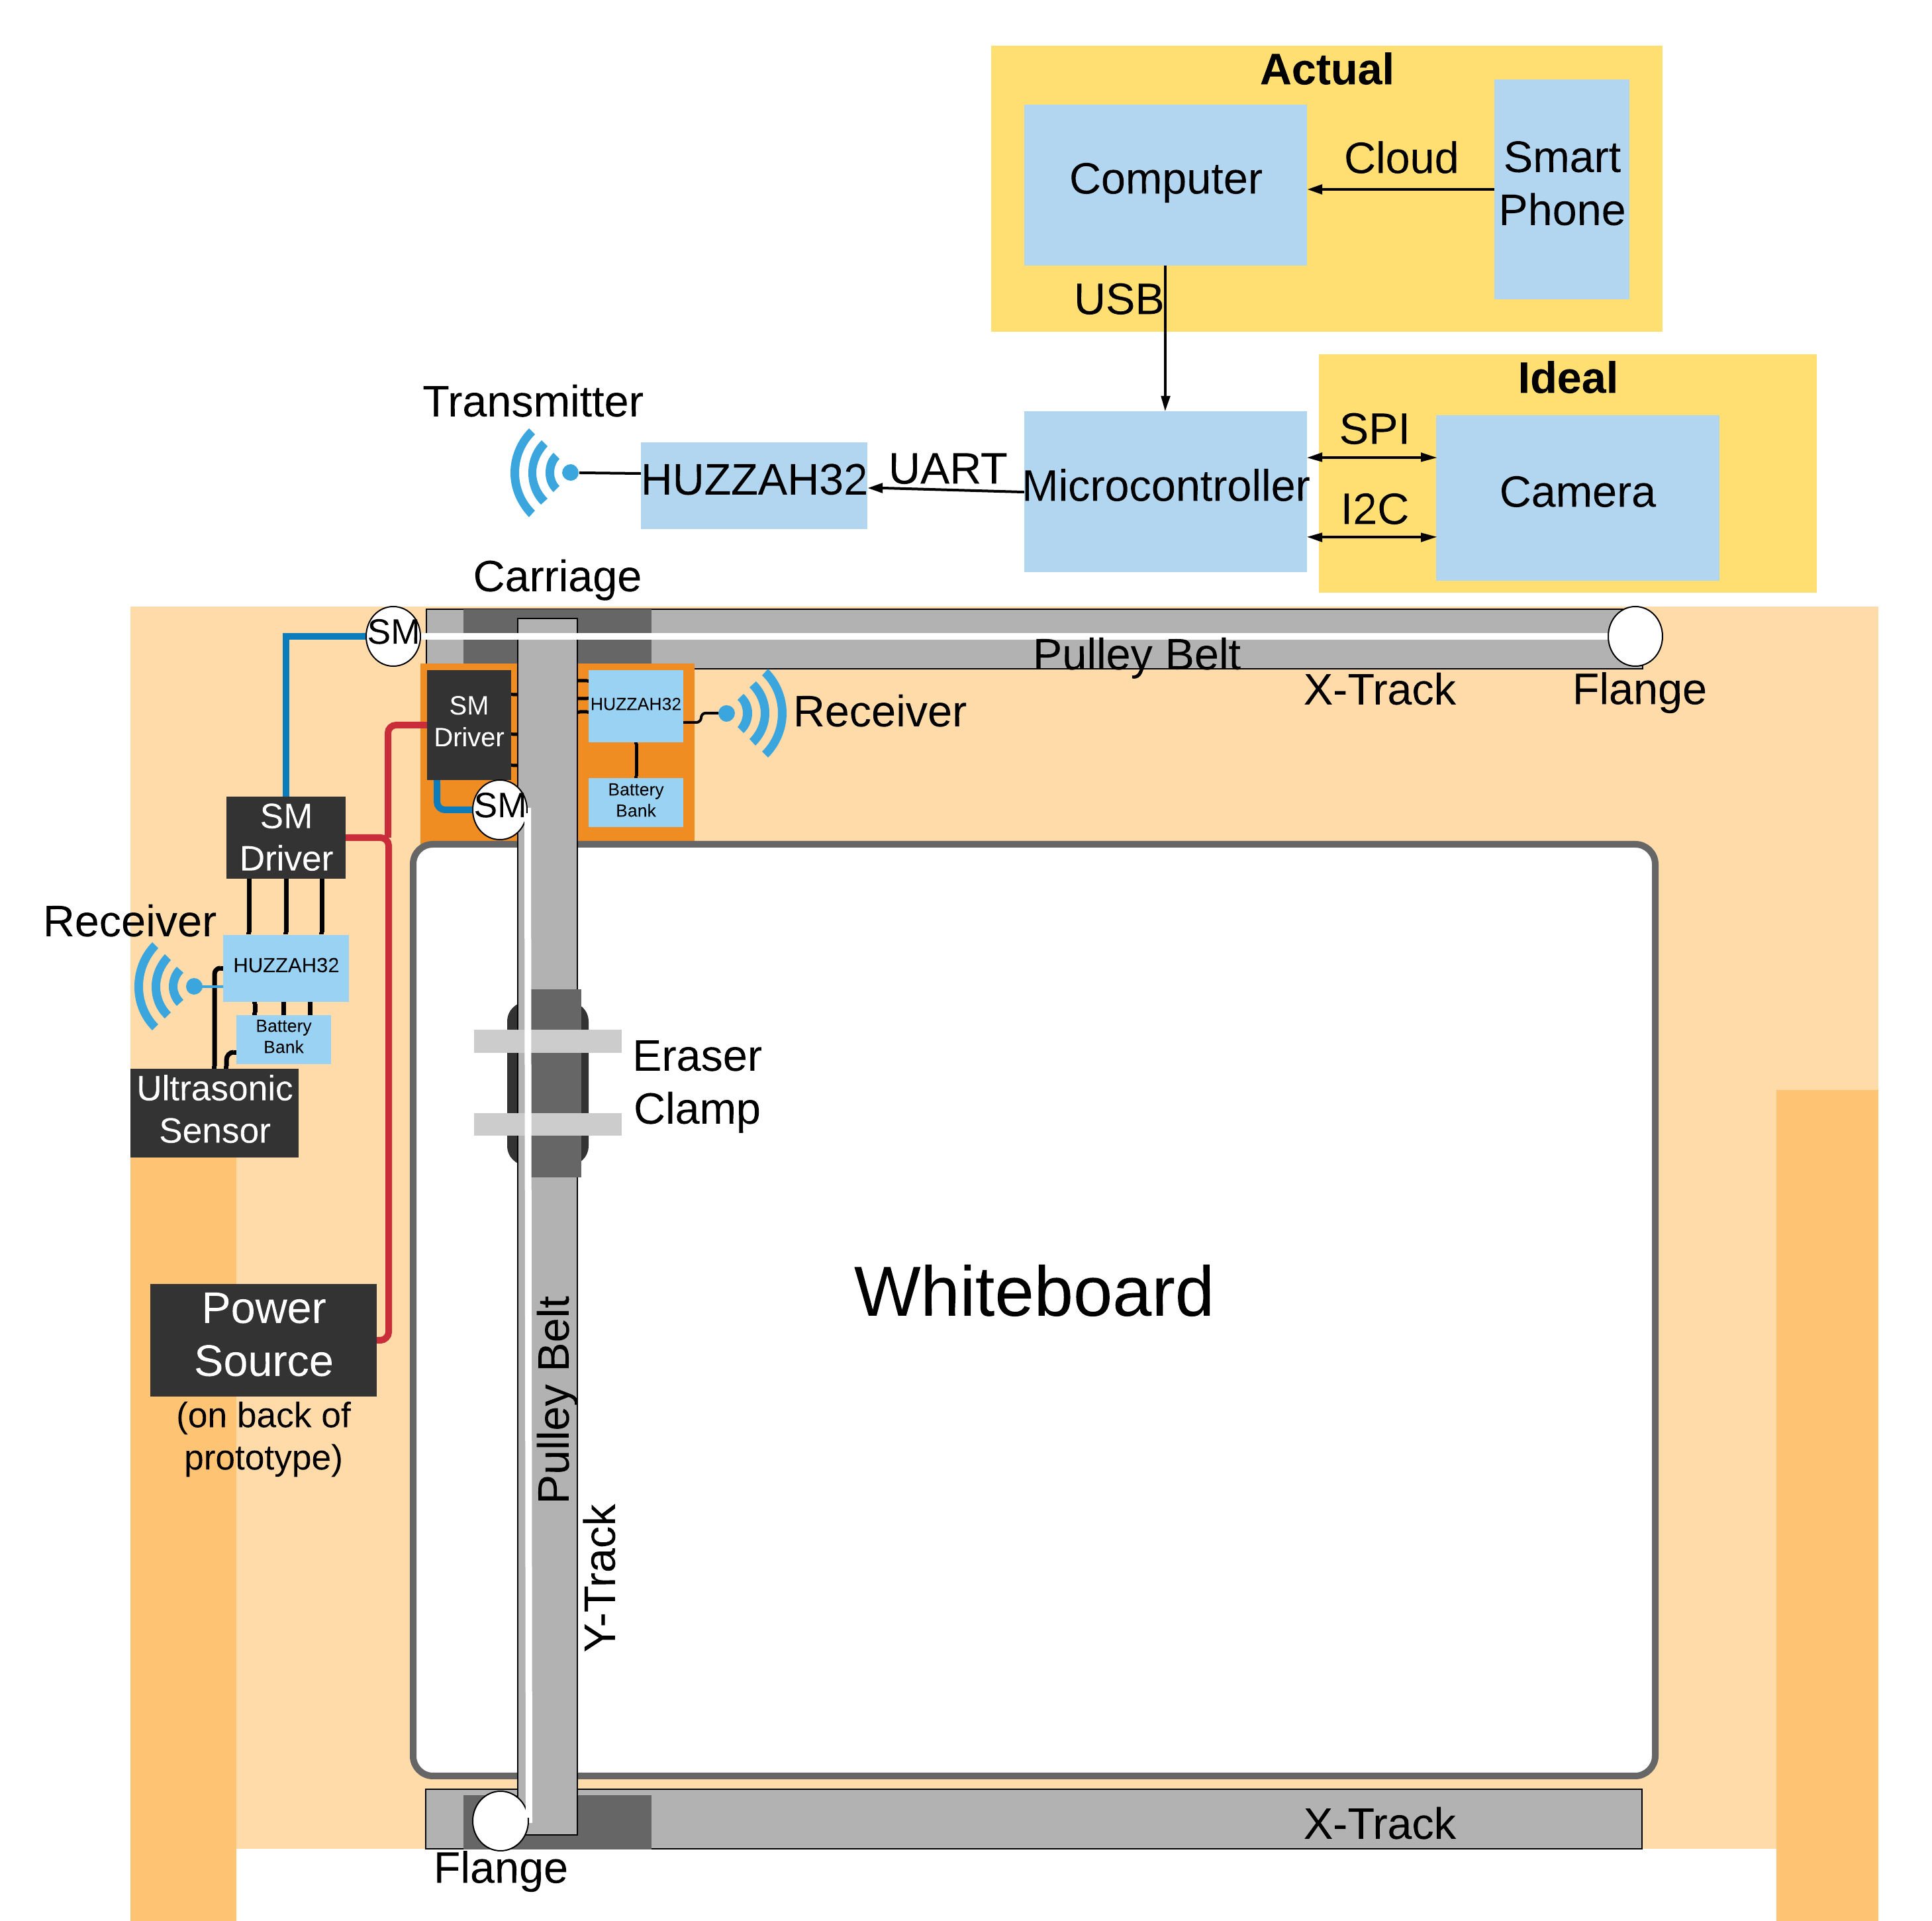
\includegraphics[max size={\textwidth}{\textheight}, scale=0.9]{Images/designOverview.png}}
	\caption{Design overview of the final product}
	\label{fig:rough}
\end{figure}

Figure~\ref{fig:rough} shows an overview of the final deliverable's mechanical and electrical components assembled with names of each item. These components and a small description of their role are listed next. For a more detailed description of each component and its role, see the \textit{Project Description and Boundaries} section of this report.

\begin{itemize}
	\item \textit{Camera}: the Arducam ideally would have captured an image of a predefined (fixed) area on the whiteboard.
	\item \textit{SPI}: Serial Peripheral Interface is one of two communication protocols that would have been used to communicate with the camera through the microcontroller and trigger a capture of an image.
	\item \textit{I\textsuperscript{2}C}: Inter-Integrated Circuit is the other of two communication protocols that would have been used to initialize the resolution and compression type of the image that is being captured by the camera.
	\item \textit{Smart Phone}: the device that takes an image of the whiteboard for the image processing program.
	\item \textit{Cloud}: the method of transferring the image taken by the smart phone to the computer that changes its format.
	\item \textit{Computer}: the system that changes the dimensions and format of the image in order to prepare it to be processed by the microcontroller.
	\item \textit{USB}: the method of transferring the newly cropped and formatted image to the microcontroller.
	\item \textit{Microcontroller}: the PSoC 6 microcontroller receives the image of the markings on the whiteboard and performs image processing to turn the image to grayscale, then uses sobel edge detection to convert where there are markings on the whiteboard to an array of 0s and Fs (with 0s representing black, blank space and Fs representing white, marked space). It then traverses the array of edges that have been detected and finds the top-most, left-most, bottom-most, and right-most locations of the markings. These four values are put into an array that is sent to the HUZZAH32 board.
	\item \textit{UART}: serial communication protocol that transfers instruction data between the microcontroller and the HUZZAH32, which sends the instructions to the stepper motors.
	\item \textit{HUZZAH32}: acts as an intermediary device for the microcontroller and the stepper motors, and acts as the wireless transceivers that allow wireless communication of information between the PSoC 6 board and the stepper motors.
	\item \textit{Transmitter}: also known as the server, reads in the stepper motor instruction array of top-most, left-most, bottom-most, and right-most values from the microcontroller and sends them sequentially to the stepper motors via a wireless connection.
	\item \textit{Receiver}: also known as the client, receives the instructions sent by the transmitter and uses an algorithm to create a serpentine-like path from the instructions that the stepper motors will understand and follow. The receiver also controls the stepper motor movement itself.
	\item \textit{Battery Pack}: mobile battery unit that is used to power the HUZZAH32s on the receiving end.
	\item \textit{SM}: stepper motors that allow the eraser to move in the X and Y axis directions. The stepper motors are connected to flanges on the opposite side of their axes with a pulley belt to allow movement.
	\item \textit{SM Driver}: regulates the voltage, current, and rotation instructions for the stepper motors, allowing them to move the way they should with little to no risk of burnout.
	\item \textit{Flange}: connects to the stepper motors via a pulley belt in order to allow movement.
	\item \textit{Pulley Belt}: the belt that wraps around the flange on the stepper motor and the other flange attached opposite to the stepper motor that moves the system.
	\item \textit{Carriage}: component within the track that actually moves back and forth. The carriage connects to the pulley belt that runs between the stepper motors and the flanges via washers and nuts. This connects the devices that need to move to the parts that do the movement.
	\item \textit{X-Track}: the two tracks that allow the eraser to move in the X-axis direction.
	\item \textit{Y-Track}: the track that allows the eraser to move in the Y-axis direction.
	\item \textit{Eraser Clamp}: metal braces and brackets that clamp to the eraser and connect it to the Y-axis carriage in order to move it.
	\item \textit{Whiteboard}: surface that is written on and erased.
	\item \textit{Power Source}: an extra power source, besides the battery packs, which is attached to the back of the finished system. It is used to power the stepper motor drivers, and in turn, also powers the stepper motors themselves.
	\item \textit{Ultrasonic Sensor}: sensor that detects changes in proximity to it. It is used as a safety precaution to those who may be standing too close to the board while it is moving.
	\item \textit{Neopixel LEDs}: LEDs connected to the ultrasonic sensor that flash green when no one is close to the board, and red when someone is standing too close to it.
	 
\end{itemize} \par
\subsection{Work Distribution}
\setlength{\parindent}{2.5ex} Heather Libecki was responsible for being the project manager of the Smart Eraser project. She was in charge of the stepper motors and all of their various components, including their drivers, and connection between the motors and the microcontroller, as well as the code that was written to move them. She also created the wireless connections between the receiver stepper motor HUZZAH32 boards and the transmitter HUZZA32 board. She also had Chris' assistance with writing the code for the wireless communication, as he was more experienced with Micropython. Finally, she was in charge of the algorithms used to find the outer-most edges of the markings on the board based on the array Chris got after processing the image, and using these to create instructions for the stepper motors so it would move the eraser to the markings found on the whiteboard, and erase them in a serpentine-like pattern before moving back to its standby position. Therefore, she was in charge of the setup of the stepper motors, the movement of the Smart Eraser, and the wireless communication between the receiver HUZZAH32 attached to the stepper motors and transmitter HUZZAH32, which got the instructions to where they needed to go. \par
\setlength{\parindent}{2.5ex} Chris Quesada was in charge of the research into and understanding of the PSoC 6 microcontroller, including its comprehensive Integrated Development Environment (IDE). He was then responsible for developing a working SPI and I\textsuperscript{2}C communication between the PSoC 6 and the camera that was ideally going to be used. The I\textsuperscript{2}C communication was used to configure the image sensor to output RGB565 with a 320x240 resolution, and the reading of the image data was done with SPI. After an image was received, he developed an image processing program which takes in an image, converts it to grayscale, then uses a sobel edge detection algorithm to detect edges of objects in the image. To know if this algorithm worked correctly, he had to set up the PSoC 6 to display images on the included TFT display. He headed the creation of the UART communication between the HUZZAH32 and the PSoC 6 with assistance from Juan. To allow for easier program management, he was in charge of adding virtual memory to the PSoC 6 to allow for an entire image to be processed, rather than parts of the image. Therefore, he was in charge of the image processing brain behind the Smart Eraser, configuration of the PSoC 6 hardware, graphical display of image, addition of virtual memory, and any wired communications to and from the PSoC 6.
 \par
\setlength{\parindent}{2.5ex} Juan Colin was in charge of the initial conception, design, and execution of the physical mechanical system and its interconnections. He was also in charge of drafting and making the wooden prototype stand and mounting all of the components together so as to ensure spacial efficiency and visual impact. He also assisted in setting up the Arducam via an Arduino platform to analyze the SPI and I\textsuperscript{2}C signals being sent from the camera. He also created a program on one of the HUZZAH32 boards that would connect to an ultrasonic sensor in order to detect if people were standing to close to the whiteboard while it is moving. Therefore, he was in charge of the entire physical prototype construction of the Smart Eraser, as well as the safety precautions advertised by the board to those around it.
 \par
\setlength{\parindent}{2.5ex} During the project's life cycle, there were a number of deliverables that needed to be submitted to Dr. Stillmaker which were worked on by all three members to ensure a consistent flow of information throughout all written documentation, including the Project Charter and this report.

 \section{Project Objectives and Success Criteria}
This section describes the objectives of the Smart Eraser. A more detailed description of the project can be found in the \textit{Project Description and Boundaries} section of this report.
\subsection{Main Objectives}
The main objectives the Smart Eraser have are listed next.
 \begin{itemize}
 \item Create a functioning mechanical system that allows the eraser to move in the x and y plane in order to erase the entire whiteboard.
 \item Create a functioning Smart Eraser that erases detected markings in a timely manner.
 \item Create an image processing program to detect said markings on the whiteboard.
 \item Create a coordinate system based on the processed image to move the eraser to specific markings.
 \item Create an algorithm to determine a path for the stepper motors to take in order to eraser all markings.
 \item Create a motion-detection program to check for people too close to the whiteboard while the system is in motion.
 \end{itemize} \par

\subsection{Simple success criteria}
\setlength{\parindent}{2.5ex} The specific criteria that need to be met in order to consider this project a success are listed next. These criteria help to measure the success of the final product. Simple success criteria are first listed which describe the tangible goals for the project to be considered a success. Then more ambitious success criteria that describe a more ideal version of the project are listed, which include additional features that would have been added if there was more time after the completion of the simple success criteria.\\

\subsubsection{Completed}
\begin{itemize}
\item The tracking system moves the eraser to all parts of the whiteboard.
\item Eraser erases the entire whiteboard with no smart processing.
\item Location of markings in an image are found through an edge-detection image processing program.
\item Image captured can be processed to find markings on board.
\item Array with locations of markings can be converted to stepper motor rotations to move eraser to proper destination.
\item Image processing program on microcontroller works with the image taken to find the markings on the whiteboard.\\
\item Motion detection is utilized for safety precautions to warn those standing too close to the whiteboard.
\end{itemize}
\subsubsection{Not Completed}
\begin{itemize}
\item Shortest path determined through Dijkstra's analysis of the array with the marking locations.
	\begin{itemize}
	\item This was unable to be completed within the allotted time. An alternative algorithm that erases the markings within a boundary in a serpentine-like pattern was used instead.
	\end{itemize}
\item Camera connects wirelessly to the microcontroller then stores it to its SDRAM.
	\begin{itemize}
	\item It was determined that the hardwired camera prototype needed to be abandoned; because of the outputted format of the camera to the microcontroller being JPEG rather than RGB565, the connection between the two wound up being more complicated than originally anticipated. The ``camera'' wound up being a smart phone image which was cropped, converted to RGB565 format, then sent into the image processing program.
	\end{itemize}
\end{itemize}

\subsection{Ambitious success criteria}
Ambitious success criteria detail functionalities that would have been completed if there was more time to work on the project.\\
\subsubsection{Completed}
\begin{itemize}
	\item Unfortunately, because not all of the simple success criteria were completed, none of the ambitious success criteria were able to be started.\\
\end{itemize}
\subsubsection{Not Completed}
 \begin{itemize}
 	\item Phone or tablet application that shows a live feed of the whiteboard from the camera
 		\begin{itemize}
 		\item Application can send specific coordinates to the whiteboard to ``pick and choose'' what section of the board to erase.
 		\end{itemize}
 	\item Attachable spray system applies whiteboard cleaning liquid solution to perform ``full clean'' of whiteboard.
 		\begin{itemize}
		\item Timer tells eraser to perform a ``full clean'' during the night when no one is using the classroom.
		\end{itemize}
 	\item Eraser can be raised off of whiteboard surface and subsequently re-pressed onto the board as needed.
 	\item Store images each time the board gets erased to provide the teacher with the class notes for the day.
 	\item Add remote control capabilities to control eraser at-will.
 	\item Smart Eraser patent.
 \end{itemize}

 \section{High-Level Requirements}
The high-level requirements associated with the completion of this project are outlined in the following list. \par
\setlength{\parindent}{2.5ex} The project should:
\begin{itemize}
\item Be completed within the outlined budget.
\item Be implementable within 2 semesters.
\item Be complex enough to warrant the title ``senior design project''.
\item Produce a complete Project Charter outlining the various project information, figures, and tables of the Smart Eraser.
\item Have significant, roughly equal portions of the project be completed by each team member.
\item Utilize material learned in core and technical elective classes throughout college careers.
\item Produce a Final Project Report outlining all information needed to be met for the project, as well as all analysis, design, and result information received during the completion of the project.
\item Produce a deliverable that can be presented in the Senior Project Presentation Day event held in the Satellite Student Union building.
\end{itemize}

\section{Assumptions, Constraints, and Standards}

This section outlines the various assumptions that were made for the requirements of this project based on previously learned course information, the constraints the project had during its conception, and the standards that were used and followed throughout the completion of this project.\par

\subsection{Assumptions}
The Smart Eraser was the first large-scale project that the students involved had worked on. Therefore, there were many assumptions made about the components that would be used to complete it, the skill-set and course information needed to complete it, and the amount of time it would take to actually complete the project. Some of the major assumptions made that wound up not being followed included the budget outlined, using the DE1\_SoC microcontroller for the main brain behind the Smart Eraser, using the Raspberry Pi microcontroller with wireless transceivers for the wireless communications, and the amount of time it would take to put together the wireless communication system. Because the first attempt at creating the wireless system ended in failure, a new system had to be conceptualized and created from scratch with 3 weeks left before the due date of the final working product.

\subsection{Constraints}
A few of the constraints foreseen at the beginning of the project were the additional power supplies needed to make the stepper motors and their drivers operate without having to constantly change batteries, and how the power is supplied to the system, especially the moving components. These were solved with an additional power supply and a long cord going to the stepper motor drivers and a battery pack for the moving HUZZAH32 board.

\subsection{Relevant Information Learned from Past Courses}
The following list outlines the relevant courses and the material they contain that were used throughout the project's lifecycle.\par
\begin{itemize}
\item ECE 70 - Engineering Computations
	\begin{itemize}
		\item C programming 
	\end{itemize}
\item ECE 85 - Digital Logic Design 
	\begin{itemize}
		\item Developing PCB for stepper motor connections
		\item Any state diagrams needed for logic between processes
	\end{itemize}
\item ECE 90 - Principles of Electrical Circuits
	\begin{itemize}
		\item Developing the power scheme and parameters for the stepper motors, stepper motor drivers and track system
	\end{itemize}
\item ECE 106 - Switching Theory and Logical Design
	\begin{itemize}
		\item Developing flow charts and block diagrams of the overall system
	\end{itemize}
\item ECE 118 - Microprocessor Architecture and Programming
	\begin{itemize}
		\item Recursion programming and algorithms developed for shortest path
		\item Determining how to store memory in a microcontroller
		\item Working with GPIO connectors on a microcontroller
		\item Using stepper motors, their drivers, and an additional power supply to operate the motors with a microcontroller
		\item Programming push-buttons on a microcontroller
	\end{itemize}	
\item ECE 122L - Micropython Lab
	\begin{itemize}
		\item Setting up the wireless communication on the specific HUZZAH32 microcontroller board chosen to be the wireless transceivers for the stepper motors.
		\item The Python language that is used to program the HUZZAH32 microcontroller board.
	\end{itemize}
\item ECE 146 - Computer Networks
	\begin{itemize}
		\item Wireless connection between systems and how data is transferred over this connection
	\end{itemize}
\item ECE 174 - Computer Architecture and Organization
	\begin{itemize}
		\item Knowing how memory is set up and the different methods of accessing it for the storage and access of the image taken from the camera.
	\end{itemize}
\item ECE 178 - Embedded Systems
	\begin{itemize}
		\item Development of algorithms
		\item Basic foundation of and general layout of hardware in microcontrollers, as well as the IDE that is specific to it
		\item Interfacing with peripherals on the microcontroller
		\item UART, SPI and I\textsuperscript{2}C communication
	\end{itemize}
\end{itemize}\par
 
Based on the courses provided in the previous list, the following information was extracted from the knowledge gained while taking these classes over the last 3-4 years. Because the following information is from notes taken during these courses, there are no sources provided for where it was learned. More in depth research obtained from external sources and their references are located in the \textit{Project Description and Boundaries} section of this report.\\

\subsubsection{Data Storage}
The images taken from the camera need to be saved to the microcontroller in order to allow the image processing program to access them. Due to knowledge gained from the \textit{Computer Architecture and Organization} class, attempts at adding memory were made in order to account for the minimal memory provided by the 1 MB of flash. However, after ample time was spent trying to get it to work, this was abandoned in order to focus on delivering a working prototype that met our simple success criteria. Because virtual memory was not able to be added, only the flash memory was used to run our entire system which led to design changes in our algorithms. For example, only 80 rows of pixels could be stored in an array during a given processing cycle. This means that one-third of the image is processed at a time and then overwritten by the next one-third instead of being able to process all image data at once.\\
\subsubsection{Translate Detected Markings into Coordinate System (Stepper Motor Rotations)}
Through team collaboration, it was decided that each stepper motor rotation would represent one pixel length. This is how a coordinate system can be developed. For example, if the image processing algorithm picks up a mark that is 56 pixels from the left of the image, and 178 pixels from the top of the image, this would result in 56 partial rotations to the right on the x-axis motor and 178 partial rotations down on the y-axis motor. Further testing determined the partial angle of rotation needed to represent one pixel length, and is discussed further in the \textit{Stepper Motor Movement} sub-subsection of \textit{The Current Wireless Communication System} subsection of the \textit{Analysis and Design} section of this report. In order to line up the physical layout of the board with a 320x240 image window, indicators are placed on the board in order to know where the image area actually is.\\
\subsubsection{Stepper Motor System Design}
The stepper motors themselves have 6.35mm teeth bore flanges. These ``teeth'' are used to grip the pulleys that drive the movement of the linear motion system. In order to rotate the stepper motors. Specific stepper motor drivers (DM542T) are used in order to drive them. This stepper motor ``system'' is designed on a PCB in order to minimize odd connections and loose wires in the final product. Also attached to these stepper motor system's PCBs are an Adafruit HUZZAH32 Feather Board microcontroller that receives the instructions needed to make the stepper motors rotate the desired distance.\\
\subsubsection{Microcontroller Involvement}
The process of learning the hardware and IDE of a microcontroller, which was gained from the Embedded Systems course, was implemented with the PSoC 6 microcontroller. Their IDE, Modus Toolbox, is an all-in-one hardware configurator, debugger, and program downloader that is based off Eclipse. The hardware configuration is very straightforward when compared to other programs like Quartus and makes developing and implementing a system much easier with everything in one place. The programs are written in C and any hardware designs that are generated create structures that can be used with provided API's(functions and macros) in order to interact with said hardware. Development of the C programs used in the system took experience gained from the Engineering computations class to employ modular programming and a more optimized flow. \\

\subsubsection{Shortest Path Algorithm}
The original plan to create a shortest path algorithm came from the knowledge of Dijkstra's algorithm gained from the \textit{Computer Networks} course. This idea was abandoned, however, due to the time constraints on the project. An algorithm that finds the outer-most edges of the markings on the whiteboard, then erases the markings in a serpentine-like pattern was chosen instead.\\

\subsubsection{Image Processing}
One of the main components of the Smart Eraser is its image processing capabilities. The PSoC 6 is fed an image through a wired SPI and I\textsuperscript{2}C communication with the camera and store that image in memory. Once the image has completed its processing and the array of the image data needs to be sent to the HUZZAH32, it does so through a UART serial connection to the board. All of these methods of communication were learned in the \textit{Embedded Systems} course. The rest of the image processing algorithm and other information pertaining to it had to be researched outside of the course information learned.\\

\subsubsection{Wireless Connectivity}
The instructions for the stepper motors need to be received wirelessly from the PSoC 6. The chat room program that was assigned in the \textit{Computer Networks} course was used as a template for the wireless transmission of these instructions between the transmitter HUZZAH32 and the two receiving HUZZAH32s. This program was made with the MicroPython programming language, and was also used as an assignment in the \textit{Micropython Lab} course.\\

\subsubsection{Ultrasonic Sensor Proximity Detection}
One of the original goals for this project was to have a motion detection system to detect if a person was moving in front of the whiteboard. Rather than detecting motion, however, the ultrasonic sensor that is used in the project detects a change in proximity of an object to the sensor. Therefore, if it detects an object to be a specified distance away, it will warn the object that it is getting too close to the system. The Micropython and mechanics behind the sensor were learned about and used in the \textit{Micropython Lab} course.\\

Additional research pertaining to these topics and how they were implemented in the project are in the \textit{Project Description and Boundaries} section of this report.   

\subsection{Standards}
\setlength{\parindent}{2.5ex} Based on the components and parts that were used in this project, the following standards were found to apply, and were followed during the creation and implementation of the Smart Eraser.
\begin{itemize}
	\item IEEE 802.15.3e-2017 - IEEE Standard for High Data Rate Wireless Multi-Media Networks--Amendment 1: High-Rate Close Proximity Point-to-Point Communications
	\begin{itemize}
		\item Applies to the wireless communication and data transfer between components in the system \cite{wifiStandards}
	\end{itemize}
	\item IEEE Editorial Style Manual
	\begin{itemize}
		\item Standards to follow when writing this Project Charter and any other reports that were written for this project \cite{ieee}
	\end{itemize}
	\item NEMA Standards Publication ICS 16 Motion/Position Control Motors, Controls, and Feedback Devices
	\begin{itemize}
		\item Applies to the stepper motors being used and their operation \cite{nema1}
	\end{itemize}
	\item SPI Communications
	\begin{itemize}
		\item Defacto standard
	\end{itemize}
	\item I\textsuperscript{2}C Communications
	\begin{itemize}
		\item Defacto standard
	\end{itemize}
	\item ITU-R Recommendation BT.709
	\begin{itemize}
		\item Applies to the coefficients used in the grayscale algorithm conversion \cite{rec709}
	\end{itemize}
		\item RS232 Serial Communications standard
	\begin{itemize}
		\item Applies to the UART communication between the PSoC 6 and HUZZAH32 \cite{UARTstandard}
	\end{itemize}
\end{itemize}
 
\section{Project Description and Boundaries}
This section contains a list of the major and minor components that are used in this project, as well as a quick overview of each of these components and how they play a role in the Smart Eraser project, and some boundaries that were overcome in order to ensure the success of this project. For a more detailed description of the procedure followed and the actual implementation of each part, see the \textit{Analysis and Design} section of this report. \par
\setlength{\parindent}{2.5ex}The following lists contain the major and minor components used in this project. More details about each major component's specifications and model numbers can be found in the \textit{Equipment and Budget} section of this report.


\subsection{Major Components}
\begin{itemize}
	\item PSoC 6 Development Kit
	\item Arducam
	\item Stepper motors
	\item Stepper motor drivers
	\item HUZZAH32 boards
	\item PCBs
	\item Rechargeable 9V batteries
	\item Linear motion tracks (X \& Y direction)
	\item Linear motion carriages (X \& Y direction)
	\item Timing belt
	\item Timing belt pulley flange
	\item Eraser
	\item Whiteboard
	\item Logic analyzer
	\item Ultrasonic sensor
\end{itemize}

\subsection{Minor Components}
\begin{itemize}
	\item Wire jumpers
	\item Stepper motor mounting brackets
	\item Various screws, nuts, and bolts
	\item Wooden plywood board (for mobile prototype)
	\item Wooden frame (for mobile prototype)
	\item Wheels (for mobile prototype)
\end{itemize}

\subsection{Software Components}
\subsubsection{SPI Communication}
SPI communication is used in order to talk to the SPI interface of the Arducam-5MP- mini- plus. The PSoC 6 acts as the master and the Arducam acts as the slave. In order for successful communication between the the two, the PSoC 6 needs to send a command byte where the MSB is either a 1 for `write' or 0 for `read' and the other 6 bits represent an address in the Arducam. If the command bytes sent is a write command, the byte sent directly after is the data to be written to the register address. If the command byte sent is a read command, the byte sent directly after does not matter, often referred to as a dummy byte. The purpose of the SPI communication is to initiate captures from the image sensor and to then poll register 0x41 for a capture complete signal of 0x08. Once a capture complete signal has been read, transferring of the image data can ensue. These processes are shown in Figure~\ref{fig:spiread} and Figure~\ref{fig:spiwrite}.

\begin{figure}[H]
	\centering
	{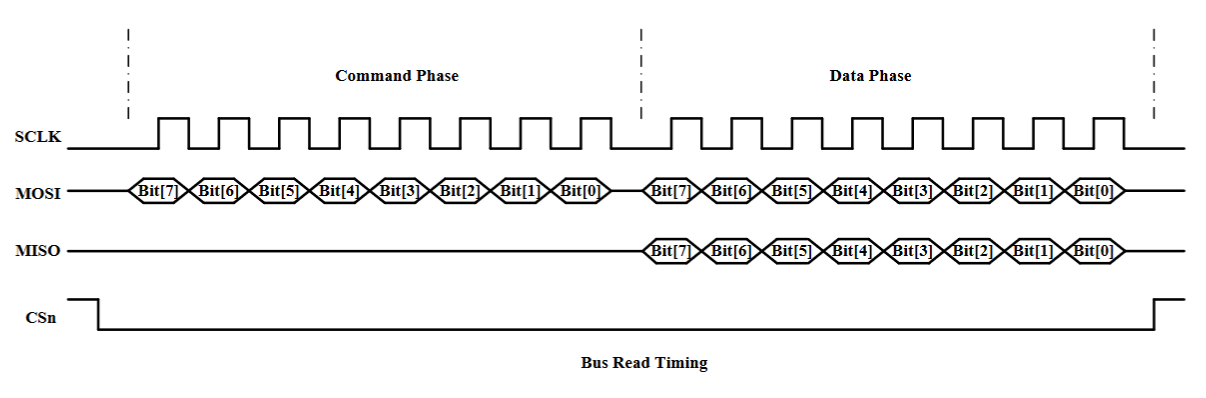
\includegraphics[max size={\textwidth}{\textheight}, scale=1]{Images/SPI_read.png}}
	\caption{Bits corresponding to a system SPI read \cite{arducam}}
	\label{fig:spiread}
\end{figure}
\begin{figure}[H]
	\centering
	{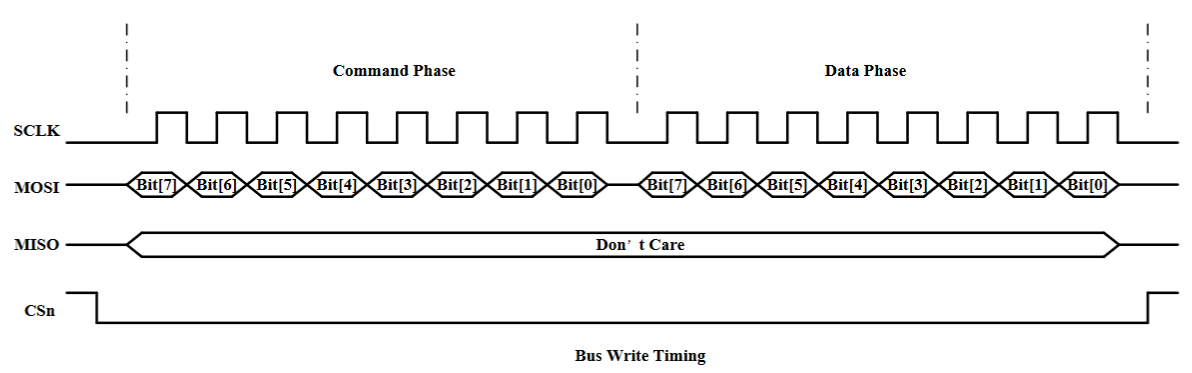
\includegraphics[max size={\textwidth}{\textheight}, scale=1]{Images/SPI_write.png}}
	\caption{Bits corresponding to a system SPI write \cite{arducam}}
	\label{fig:spiwrite}
\end{figure}

\subsubsection{I\textsuperscript{2}C Communication}
The purpose of including I\textsuperscript{2}C communication is both to initialize and configure the image sensor of the Arducam-5MP-mini-plus. The figure below provides and example I\textsuperscript{2}C exchange between a master and slave where the master is the PSoC 6 and the slave is the Arducam. The information provided from Arducam is slightly incorrect, as most developers incorrectly provide an 8-bit slave address when it should be a 7-bit. The correct address is 0x3C where a read/write bit is added on by the microcontroller. So, if its a write operation the slave address would be 0x3C plus a write-bit(0), making the slave address 0x78 (0x3C with a zero bit added onto the front of the LSB equals 0x78) and the same applies to a read operation which adds a read-bit(1). This means that there is only one slave address and not separate addresses for read and write operations.
 
 \begin{figure}[H]
 	\centering
 	{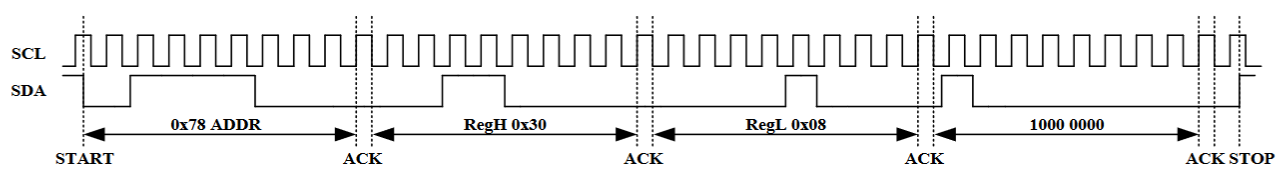
\includegraphics[max size={\textwidth}{\textheight}, scale=1]{Images/I2C_write.png}}
 	\caption{Bits corresponding to a system I\textsuperscript{2}C write \cite{arducam}}
 	\label{fig:I2Cwrite}
 \end{figure}
 
 \subsubsection{UART Communication}
The communication of choice between two micro controllers is often UART as it allows for the simplest method to communicate. Since there is no master and no slave packet transmission is done through a 1 receiver and a 1 transmitter. 
\begin{figure}[H]
	\centering
	{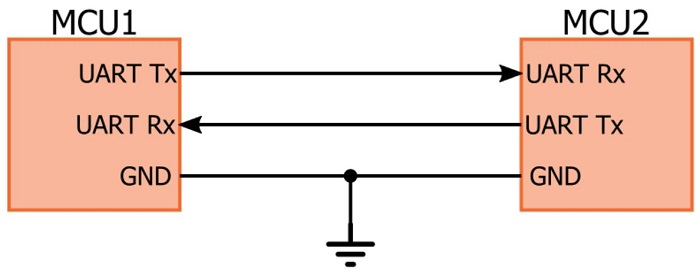
\includegraphics[max size={\textwidth}{\textheight}, scale=.85]{Images/UART.png}}
	\caption{UART Communication \cite{UARToverview}}
	\label{fig:UART}
\end{figure} 
 
 \subsubsection{Grayscale Conversion from RGB565}
 In order to detect objects in an image, the image needs to be converted from RGB to grayscale. This is because the result of the sobel detection algorithm compares light intensity changes against a threshold value. Using RGB pixel information does not provide a way for the intensities to be correctly compared because the R, G, \& B values are used to depict color and not to represent light intensity. By converting to grayscale you are creating an intensity value from the pixel information on a scale from 0-255. This can be done by using the grayscale luminance conversion algorithm which assigns weights to each value ( R, G, \& B) using coefficients from CITE BT.709 :
\begin{center}
	 $ Gray = (Red \times 0.2126 + Green \times 0.7152 + Blue \times 0.0722) $ 
\end{center}
 However, before this algorithm can be used, the red, green, and blue intensities need to be separated from the 16-bit value and shifted to an 8-bit scale, hence the name RGB565. Bits[15:11] represent red intensity, bits[10:5] represent green intensity, and bits[4:0] represent blue intensity.
 
  \begin{figure}[H]
 	\centering
 	{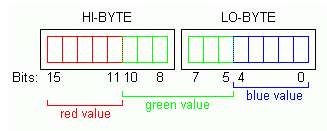
\includegraphics[max size={\textwidth}{\textheight}, scale=1]{Images/RGB565.png}}
 	\caption{How an RGB565 pixel value is stored in memory \cite{rgb565}}
 	\label{fig:rgb565}
 \end{figure}
 
 \subsubsection{Sobel Edge Detection}
 After grayscale pixels have been generated, a sobel edge detection algorithm is used in order to detect edges in an image. This is done by convolving sobel kernels, one vertical one horizontal, through the array of gray pixels. This is shown in Figure~\ref{fig:sobel}. By doing this, you can find the gradients in both the X and Y direction which is eventually be used in the Pythagorean Theorem to determine the magnitude of the gradient at that pixel location. The magnitude value is then compared against a threshold value (this threshold value can be altered to fit one's needs).
 
  \begin{figure}[H]
 	\centering
 	{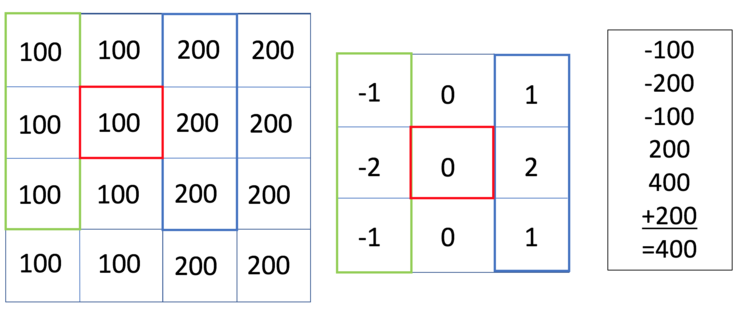
\includegraphics[max size={\textwidth}{\textheight}, scale=0.6]{Images/sobel-edge-detection.png}}
 	\caption{Kernel convolution used in sobel edge detection \cite{sobel}}
 	\label{fig:sobel}
 \end{figure}
 
\subsubsection{Socket Programming for Wireless Communication}
 Due to malfunctioning hardware concerning the Arduinos and the Kuman wireless transceivers, the original idea for the wireless communication system had to be abandoned. The new concept is to use the HUZZAH32 Feather boards as the wireless transceivers that send and receive instructions for the stepper motors to execute. These boards can be programmed with either Micropython or Arduino programming languages, but in this project, they use Micropython to perform their tasks. One HUZZAH32 board is initialized as a transmitter (server) that connect to the PSoC 6 via an UART connection and receive the stepper motor instructions, then send these instructions to the stepper motors. Two other HUZZAH32 boards act as receivers (clients); one is attached to each stepper motor, and they receive the instructions for the stepper motors. They then give them the directions to move according to the instructions received. \par
 \setlength{\parindent}{2.5ex}
 Figure~\ref{fig:socket_comm} shows an example of a client-server interaction using socket programming. First a socket connection is created between the client and server. This establishes a connection between the two entities so they are able to communicate with one another. On the server side, the socket must be bound to the server's IP address, and then issued a command to listen for incoming connections. Once the client sends a request to connect, the server accepts the command if the proper authorization is followed. In this project's case, a password and server name was created to ensure no other connections could be made to the system when it was being presented on Projects Day. After the two systems have connected, they enter a client/server session where they can communicate and send data between each other. However, once a ``close'' signal is sent to the server, or when a file has completed transmission (this depends on how the cease to connect condition is set), the server finishes reading the data sent, sees the ``close'' command, then closes the connection between the two entities. To learn more about the actual implementation of this type of programming and how it was used in the project, see the \textit{The Current Wireless Communication System} subsection of the \textit{Analysis and Design} section of this report.
 
   \begin{figure}[H]
 	\centering
 	{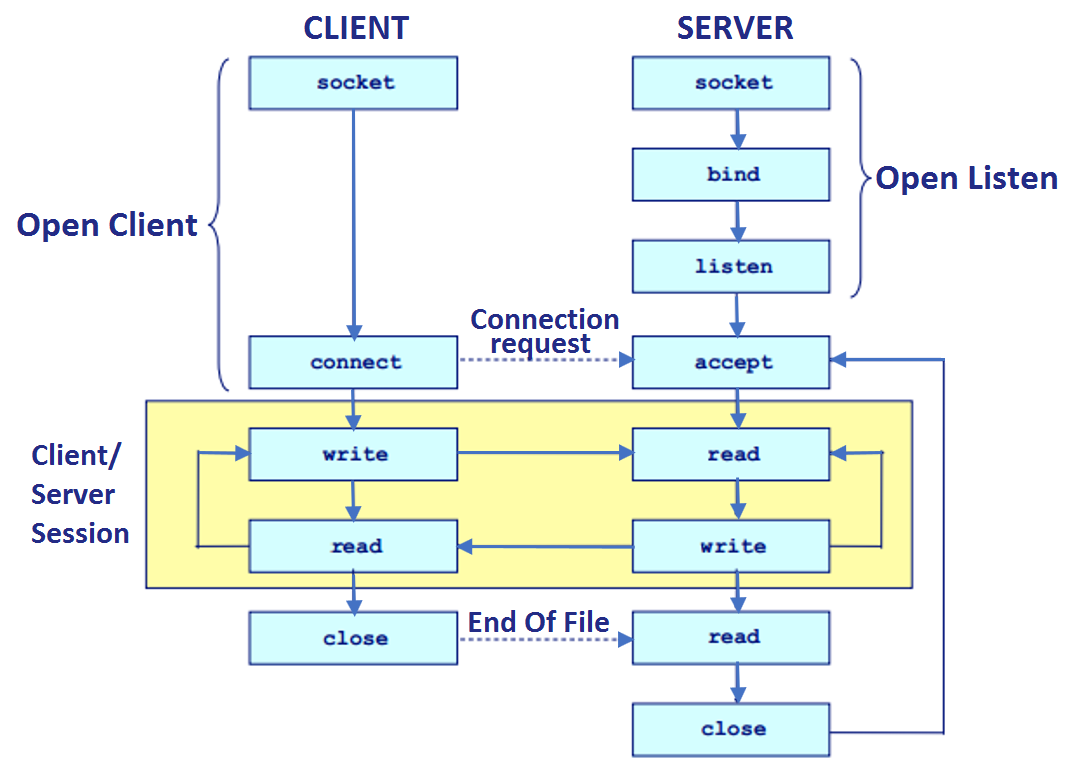
\includegraphics[max size={\textwidth}{\textheight}, scale=0.6]{Images/socket_comm.png}}
 	\caption{Socket communication protocol between server and client \cite{socket}}
 	\label{fig:socket_comm}
  \end{figure}
 
 \subsubsection{Stepper Motor Operations}
 In order for the stepper motors to move, they must be programmed to receive the correct signals at the correct time to move the magnetic coils within the motor properly. They were programmed in Micropython and connected to the HUZZAH32 boards, which provides the necessary signals to allow the motors to move. Figure~\ref{fig:smdata} shows the different steps and signals that need to be sent along the 4 leads connected to the internal magnetic coils in order to rotate them CW (clockwise) and CCW (counter-clockwise).
 
    \begin{figure}[H]
 	\centering
 	{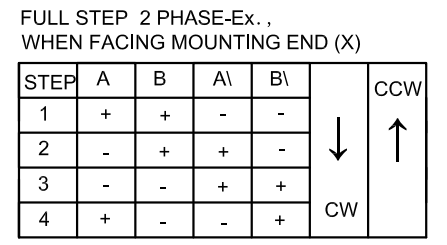
\includegraphics[max size={\textwidth}{\textheight}, scale=0.6]{Images/sm_rot.png}}
 	\caption{Rotation instructions for the stepper motor \cite{smdataR}}
 	\label{fig:smdata}
 \end{figure}
The motor moves when these steps are sent to their corresponding lead connections to the stepper motor drivers in a sequential order. The factor that determines how quickly the motors turn in the code that was written is how quickly the steps are traversed through when they are sent to the drivers. I.E., the faster they are traversed, the faster the motor will spin, and visa versa.\\
 
 \subsubsection{Moving the Eraser to the Markings}
 In order to move the stepper motors to the markings on the whiteboard, there are two algorithms: one detects the outermost edges of the markings, which essentially creates a ``square'' surrounding the markings, and the other creates a serpentine-like path within the square in order to eraser the markings. Figure~\ref{fig:serpconcept} shows the concept behind these two algorithms, if the whiteboard was divided into an 8x8 matrix. Figure~\ref{fig:squaredetect} shows the flowchart of the \textit{square\_detection.c} program that detects the square around the markings, and Figure~\ref{fig:serp} shows the flowchart of the \textit{serpentine.c} program that moves the eraser to erase the markings. \par
 \setlength{\parindent}{2.5ex}
 In order to create the correct rotation sequence for each motor, the serpentine code had to be split into two separate files for each motor and modified accordingly. For more information on this implementation, see the \textit{The Current Wireless Communication System} subsection of the \textit{Analysis and Design} section of this report.
 
    \begin{figure}[H]
 	\centering
 	{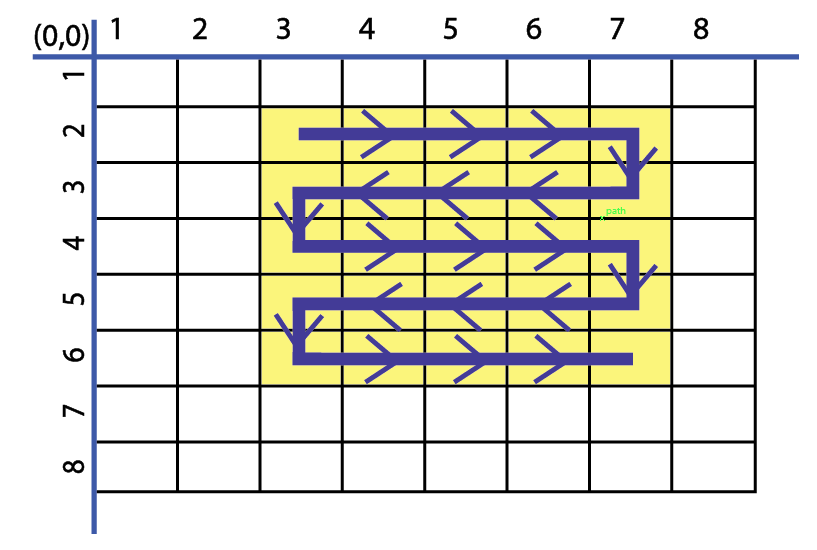
\includegraphics[max size={\textwidth}{\textheight}, scale=0.6]{Images/coordinate_algorithm_concept.png}}
 	\caption{Concept behind the two algorithms that move the eraser to the markings}
 	\label{fig:serpconcept}
 \end{figure}
   \begin{figure}[H]
	\centering
	{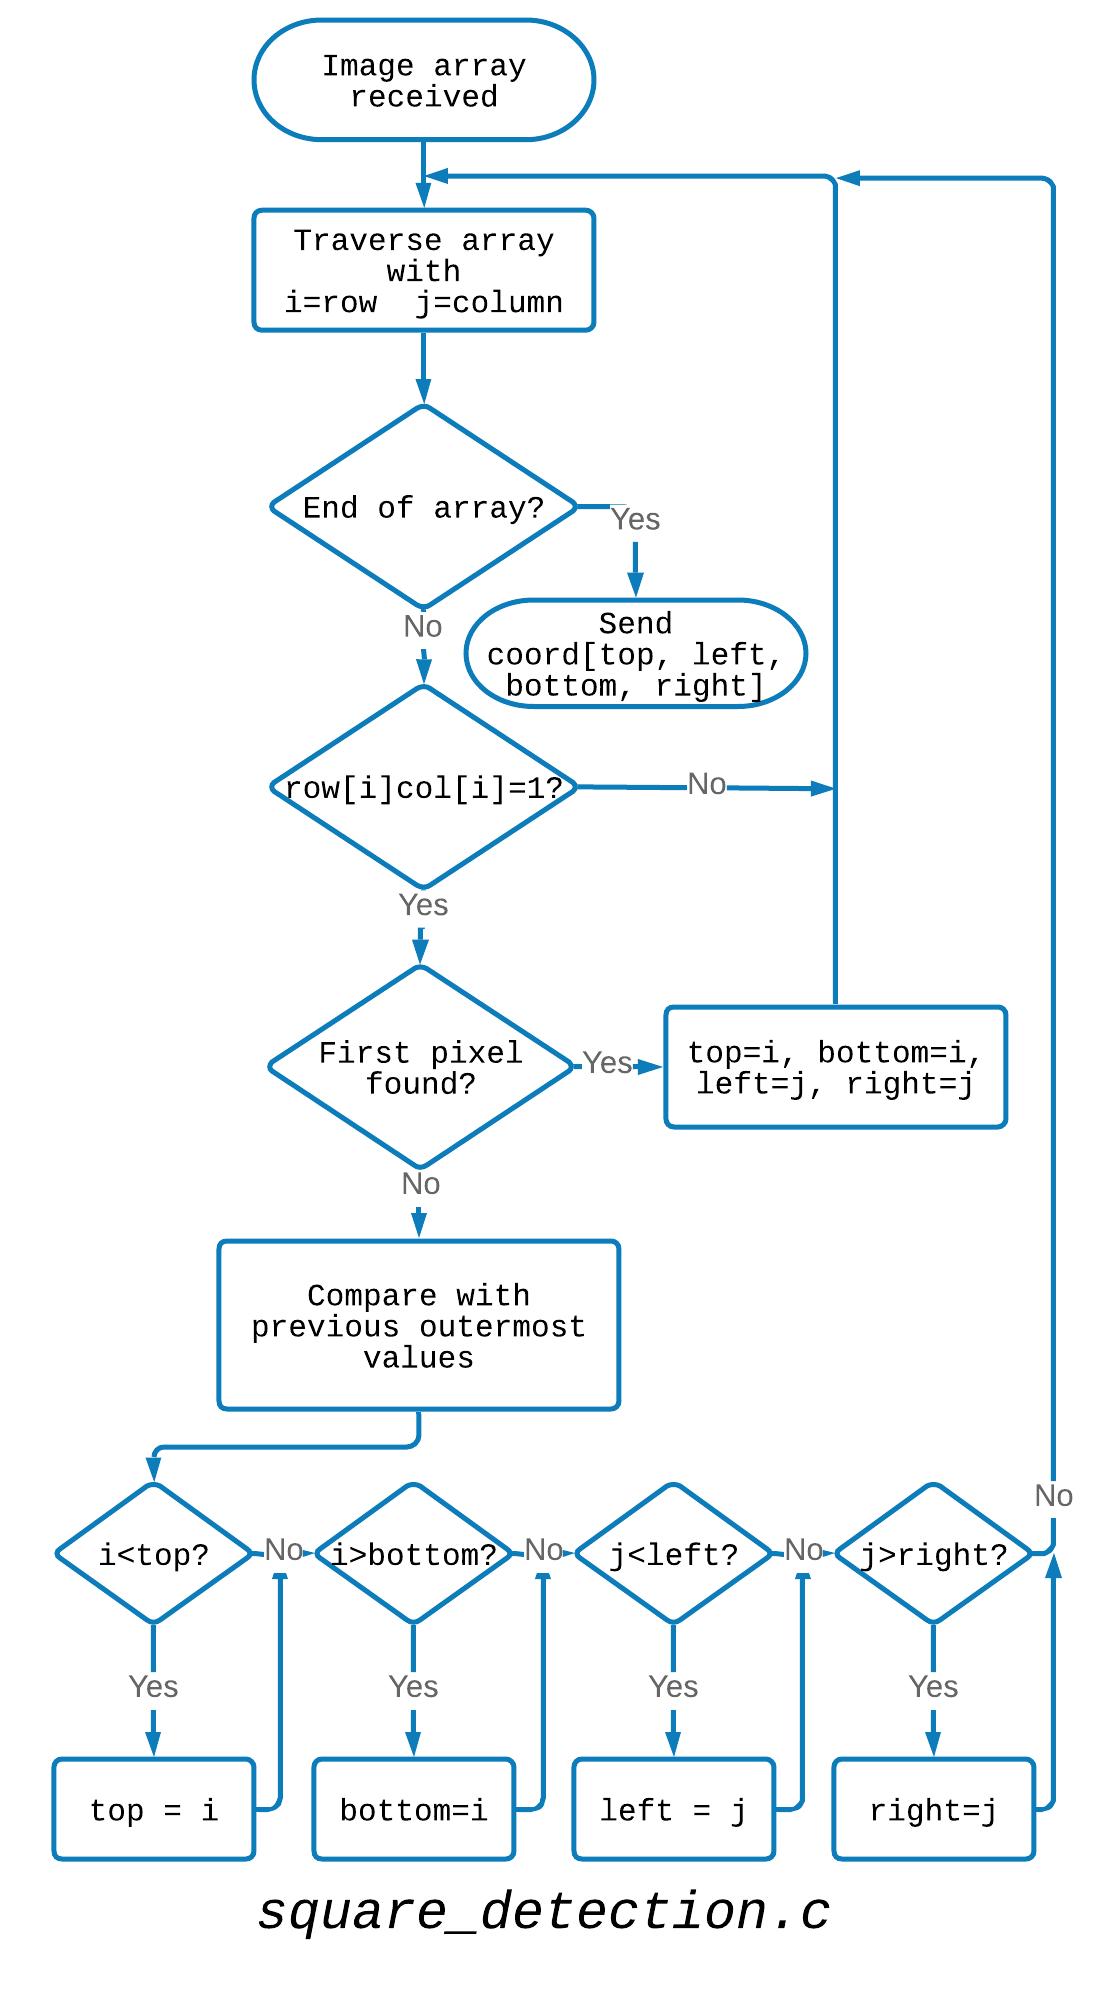
\includegraphics[max size={\textwidth}{\textheight}, scale=0.9]{Images/square_detection_c_flowchart_simple.png}}
	\caption{Flowchart of the logic behind the \textit{square\_detection.c} program}
	\label{fig:squaredetect}
\end{figure}
   \begin{figure}[H]
	\centering
	{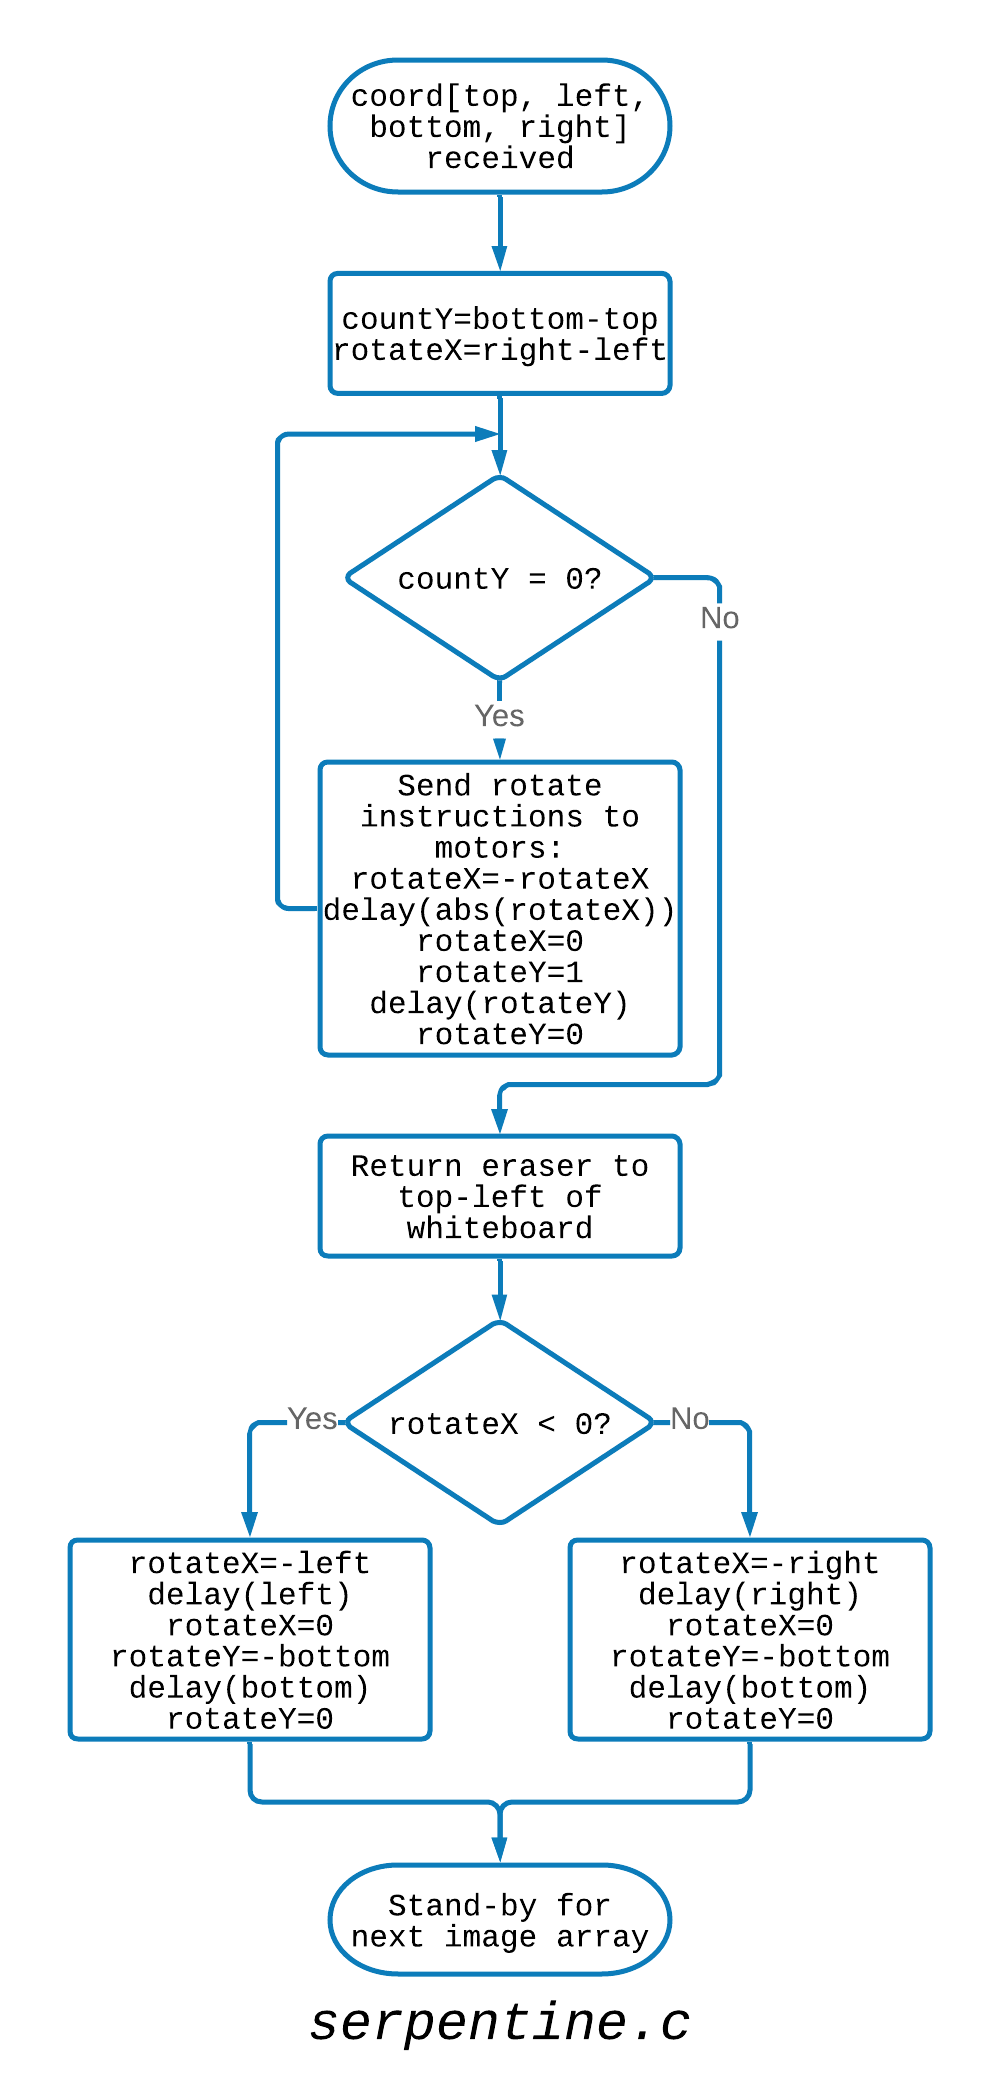
\includegraphics[max size={\textwidth}{\textheight}, scale=0.9]{Images/serpentine_c_flowchart.png}}
	\caption{Flowchart of the logic behind the \textit{serpentine.c} program}
	\label{fig:serp}
\end{figure}
 
 \subsubsection{Proximity Sensing Using the Ultrasonic Sensor}
 The Ultrasonic Sensor is able to detect changes in distance up to 4 meters. The original thought was to use these changes in distance to interrupt the eraser during its serpentine function. This was to be a safety feature but currently it only displays red if a user is too close to the board while it is erasing.
 
 \begin{figure}[H]
 	\centering
 	{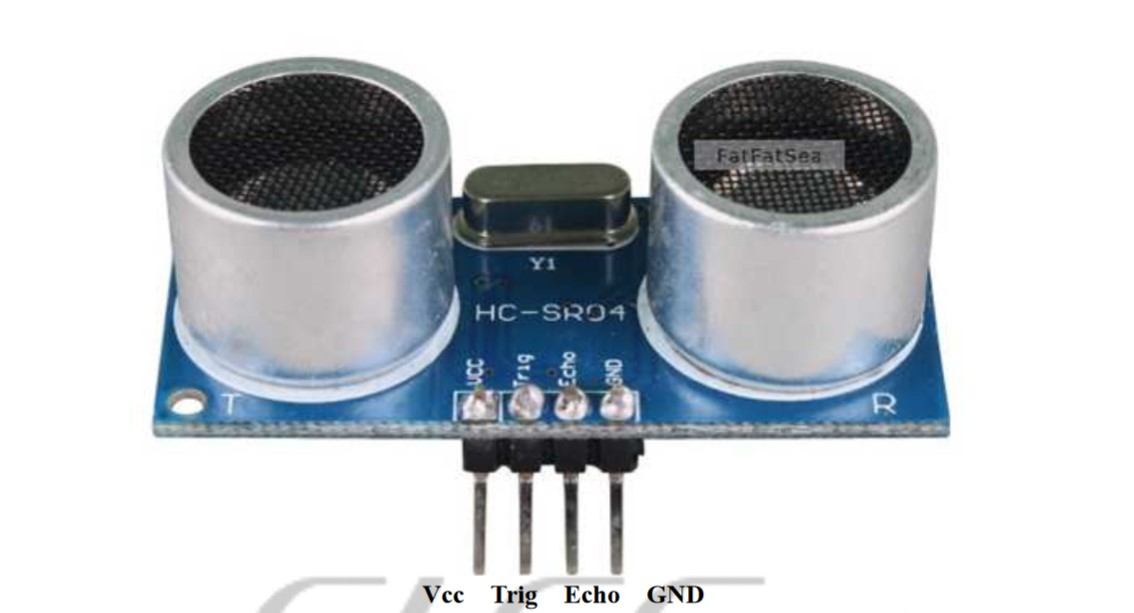
\includegraphics[max size={\textwidth}{\textheight}, scale=0.6]{Images/Ultra2.jpg}}
 	\caption{Ultrasonic sensor \cite{Ultra2}}
 	\label{fig:Ult2}
 \end{figure}
 
 \subsection{Physical Technological Components}
 \subsubsection{Arducam}
 The camera is the input that drives the functionality of the rest of the system. It provides high enough quality for future improvement, but for the purposes of this project, only a 320x240 resolution is needed. The current design has the camera directly connected to the PSoC 6 microcontroller through SPI and I\textsuperscript{2}C communication to both configure the image sensor (I\textsuperscript{2}C) and initiate data transfer (SPI). Although it is referred to as a camera it is more accurately defined as a module which has an I\textsuperscript{2}C interface to configure the image sensor and a SPI interface to handle data transfer.
    \begin{figure}[H]
 	\centering
 	{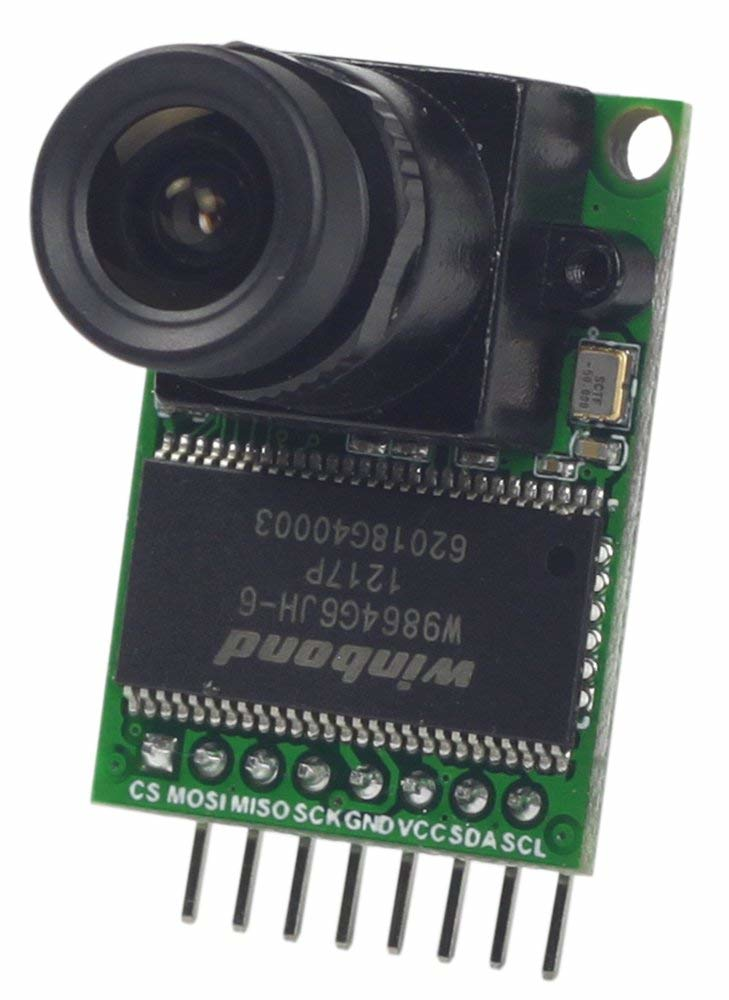
\includegraphics[max size={\textwidth}{\textheight}, scale=0.15]{Images/arducam.png}}
 	\caption{The Arducam Mini Module 5MP OV5642 Camera \cite{smdataR}}
 	\label{fig:arducamcam}
 \end{figure}
 
 \subsubsection{PSoC 6 Microcontroller}
 Due to the processing capabilities that the Smart Eraser needs to be able to accommodate, and due to the peripheral devices that need to be attached, the PSoC 6 was found to be the ideal microcontroller to use for the computations fo the mechanism. The PSoC 6 not only allows for the straightforward programming of peripheral devices attached to it, but it also has a dual -core processor built into it which can handle the programming that needs to be done for the Smart Eraser to work as intended. Within the PSoC 6 are Serial Control Blocks(SCB) which can be configured to suite the projects needs, whether it be I\textsuperscript{2}C, SPI, or UART. The SCB is the gateway to both the Arducam and HUZZAH32. There is also a TFT display attached to the microcontroller that allows for viewing of any image captured and any image processing results. Finally, SW2 is used to initiate the process from capture to erasing.
    \begin{figure}[H]
 	\centering
 	{\includegraphics[max size={\textwidth}{\textheight}, scale=0.7]{Images/psoc.png}}
 	\caption{The PSoC 6 microcontroller by Cypress}
 	\label{fig:psoc}
 \end{figure}
 
 \subsubsection{Stepper Motors}
 The stepper motors allow the eraser to move along the track and linear motion systems that are mounted to the wall above and below the whiteboard. Because of the weight of the components chosen to move along the track, a stepper motor with enough power and torque to move said components is needed. With this in mind, the NEMA 23 CNC Stepper Motor (with 1.26Nm holding torque, 1.8 degree step angle, 2.8A rated current per phase, 0.9Ω resistance, and 24-48V driving voltage) was chosen for the Smart Eraser. It is connected via jumper wires to the stepper motor drivers that allow their movement. These require additional power, and this power is supplied via three 9V rechargeable lithium batteries, which is connected through the PCB that was created for the stepper motor connections.
   \begin{figure}[H]
	\centering
	{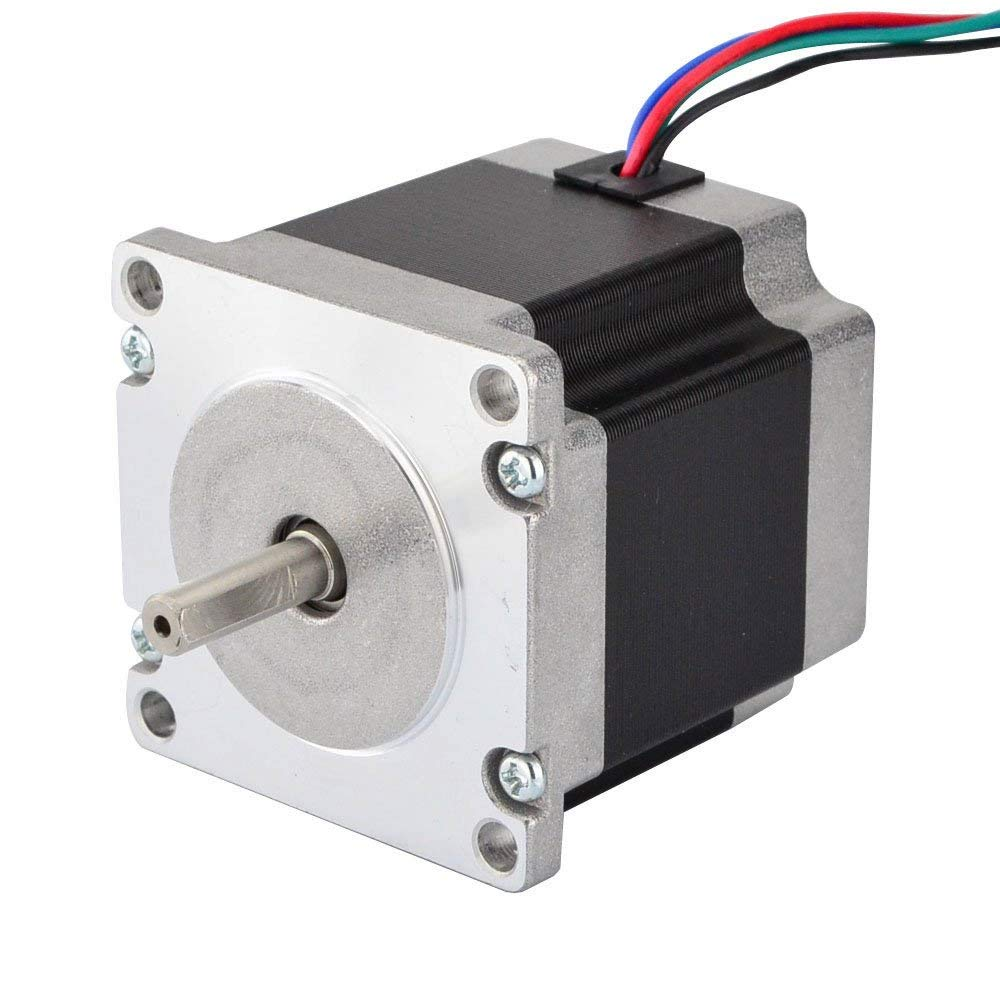
\includegraphics[max size={\textwidth}{\textheight}, scale=0.35]{Images/sm.png}}
	\caption{4-lead bipolar NEMA23 stepper motor \cite{smR}}
	\label{fig:stepmotor}
\end{figure}

\subsubsection{Stepper Motor Drivers}
The stepper motor drivers are an intermediary device between the stepper motors and the PCB. The drivers need to specifically work with the stepper motors that were chosen. Therefore, the stepper drivers that are used for the NEMA 23 stepper motors is the Full Digital Stepper Driver, model number DM542T. This model was not only chosen due to its compatibility with the NEMA 23 model stepper motors, but also because of its capabilities to drive the motors at lower noise, with lower heating, and with smoother movement. Like the stepper motors, the drivers need additional power, and they receive it through the PCB via three 9V rechargeable lithium batteries.\par
\setlength{\parindent}{2.5ex}The table in Figure~\ref{fig:smDD} shows the correct parameters for the drivers that need to be kept in mind when the additional power is connected to them via the PCB, and the table in Figure~\ref{fig:smdata} shows the specific ports that need to be driven by a high voltage value in order to allow the motor to actually rotate clockwise or counterclockwise.
   \begin{figure}[H]
	\centering
	{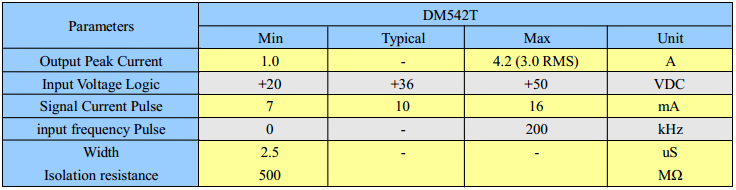
\includegraphics[max size={\textwidth}{\textheight}, scale=0.8]{Images/smDD.png}}
	\caption{Limited parameters of the DM542T stepper motor drivers \cite{smdataDD}}
	\label{fig:smDD}
\end{figure}

\subsubsection{HUZZAH32 for Stepper Motor Wireless Communication}
The HUZZAH32 by Adafruit is the main communication hardware for the stepper motors. The transmitter board is physically connected to the PSoC 6, and it contain the code to send the instructions received from the PSoC 6 to the receivers. The receivers contain the necessary code to receive the instructions wirelessly, and they also act as the controller for the stepper motors to move once they have their instructions.

   \begin{figure}[H]
	\centering
	{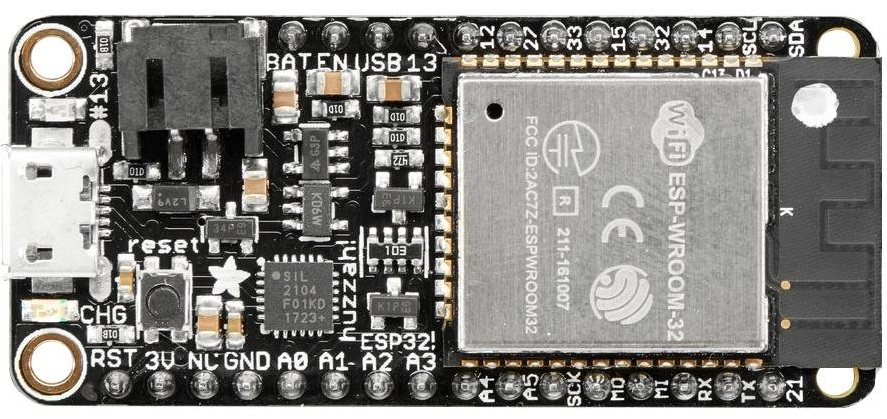
\includegraphics[max size={\textwidth}{\textheight}, scale=0.5]{Images/huzzah.png}}
	\caption{Adafruit's HUZZAH32 Feather Board with ESP32 chip \cite{huzzah}}
	\label{fig:huzzah}
\end{figure}

\subsubsection{PCBs}
The PCB (Printed Circuit Board) is an intermediary device between the stepper motor drivers and the Feather board, as well as the additional power that is needed to power the motors and their drivers. This PCB was created by the PCB design software DipTrace, and contains connecting pins to ensure spatial efficiency, as well as to make sure all components are connected properly. Due to the wireless system needing to be changed last minute, the PCB will not be used. However, because it is work that was put into the project, it will still be talked about in the \textit{Analysis and Design} section of this report.\\

\subsubsection{Additional Power}
The chosen stepper motor drivers can handle a voltage input ranging from 20 - 50 V, and the stepper motors themselves can handle a voltage input from 24 - 48V. Therefore, the power source needs to be able to drive enough current to generate that range for the stepper motors. With this in mind, the 9V rechargeable lithium batteries were chosen for the additional power source when the Arduino and transceivers were being used for the wireless communication. Three of these batteries were connected in series on the PCB to provide the additional power needed to driver the motors and their drivers. The batteries can be recharged when they are depleted, which would allow them to be reused many times for the prototype as well.

   \begin{figure}[H]
	\centering
	{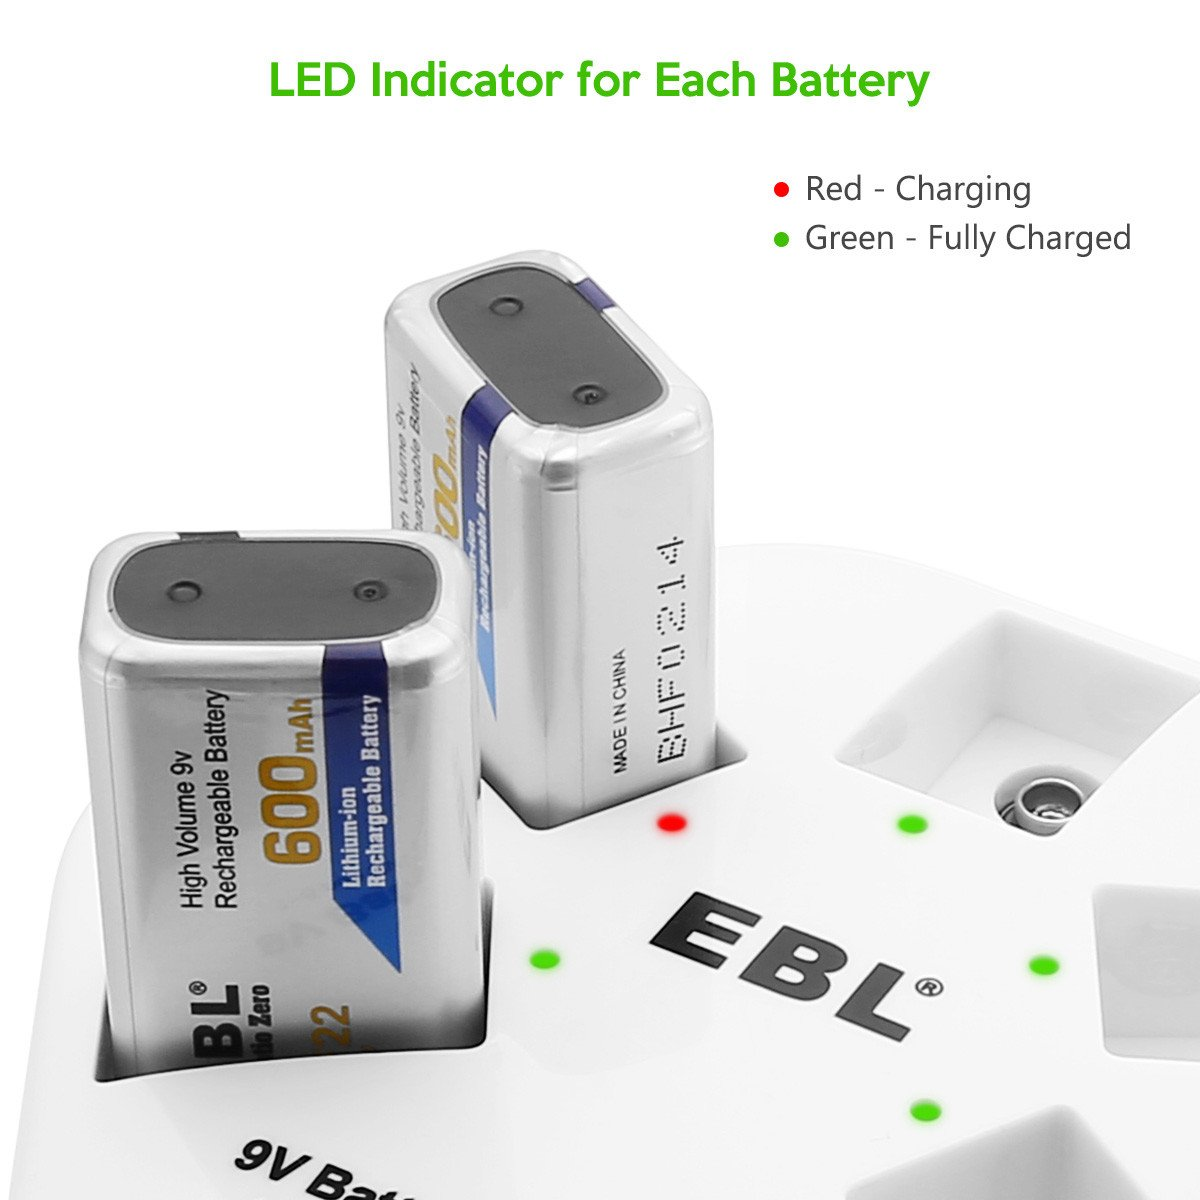
\includegraphics[max size={\textwidth}{\textheight}, scale=0.4]{Images/charger.png}}
	\caption{9V lithium rechargeable batteries \cite{ebl}}
	\label{fig:ebl}
\end{figure}

However, because the PCBs could no longer be used, additional power was gained from the TDK Lambda power supply. This supplied the stepper motors with the correct voltage.

 \begin{figure}[H]
	\centering
	{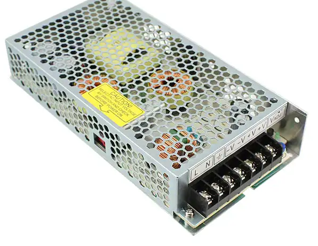
\includegraphics[max size={\textwidth}{\textheight}, scale=0.6]{Images/lambda.png}}
	\caption{TDK Power Supply used to power the stepper motor drivers \cite{supply}}
	\label{fig:supply}
\end{figure}

In order to power the HUZZAH32 boards, another type of power supply was used. A 5V battery bank was used to supply a reliable, long-lasting power supply. This was chosen with the length of Projects Day presentations in mind.

 \begin{figure}[H]
	\centering
	{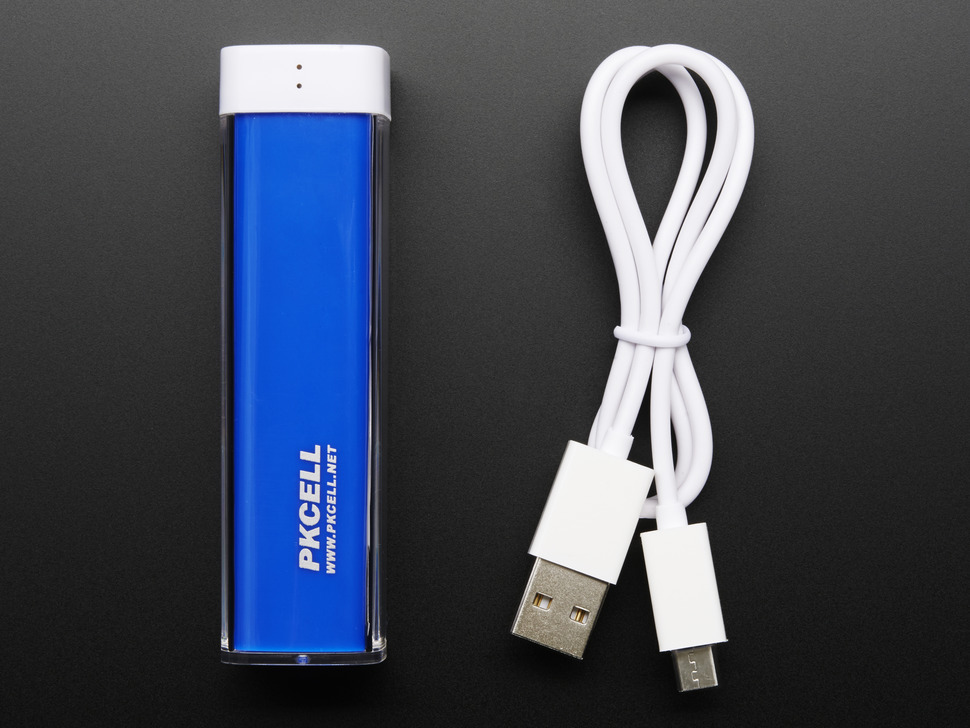
\includegraphics[max size={\textwidth}{\textheight}, scale=0.5]{Images/battery_pack.jpg}}
	\caption{Battery pack used to power HUZZAH32s reliably \cite{batt}}
	\label{fig:batt}
\end{figure}

\subsection{Physical Mechanical Components}

\subsubsection{Linear Motion Track System}

The model 115RC linear motion track system allows the eraser to move in the x-axis direction of the whiteboard. There are two tracks mounted above and below the whiteboard, and attached to the cassettes with washers and nuts is a third track that allows the eraser to move in the y-axis direction of the whiteboard. The y-axis of the tracking system was pre-drilled at both ends with a 7/32 inch drill bit in order to be placed on the m5 screw of the x-axis carriages. The y-axis was also pre-drilled with a 11/32 inch drill bit in order to attach the housing unit of the stepper motor system. The dimensions of the track systems and the carriages in them are shown in Figure~\ref{fig:accuride}.

   \begin{figure}[H]
	\centering
	{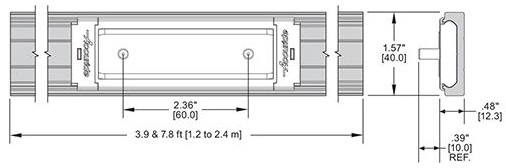
\includegraphics[max size={\textwidth}{\textheight}, scale=0.85]{Images/track.png}}
	\caption{Linear track system specifications \cite{accuride}}
	\label{fig:accuride}
\end{figure}

\subsubsection{Stepper Motor Mounts}
The stepper motor steel mounting brackets are used to actually mount the stepper motors onto the track system, as well as to lift the motors off of the wood backing enough so they are above the track. This allows the pulley system to be attached correctly.

   \begin{figure}[H]
	\centering
	{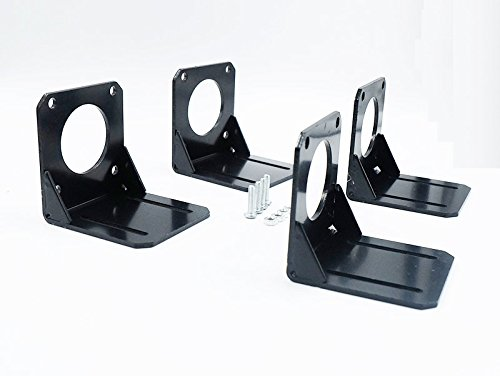
\includegraphics[max size={\textwidth}{\textheight}, scale=0.3]{Images/brackets.jpg}}
	\caption{Mounting brackets for the stepper motors \cite{bracket}}
	\label{fig:bracket}
\end{figure}

\subsubsection{Pulley System}
The pulley system consists of two components: a GT2 40-teeth 6.35 mm bore timing belt pulley flange synchronous wheel, and a 5 meter long, 6mm wide GT2 timing belt. Two pulley flanges connect to either side of the track on the x and y axes, and the timing belt wraps around them. One of the flanges on each of the axes connects to the stepper motors in order to allow the belt to actually move. The belt in Figure~\ref{fig:belt} is black in order to show the details of the teeth, but the actual belt that was used is white.

   \begin{figure}[H]
	\centering
	{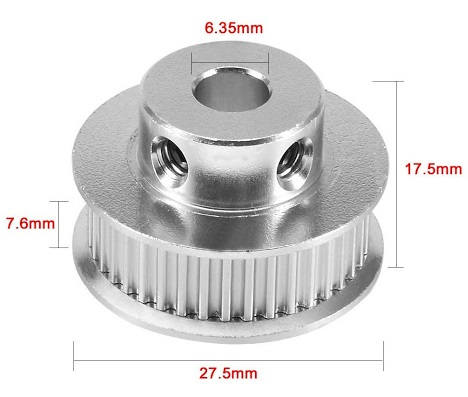
\includegraphics[max size={\textwidth}{\textheight}, scale=0.3]{Images/teeth.jpg}}
	\caption{Pulley flange \cite{uxcell}}
	\label{fig:flange}
\end{figure}
   \begin{figure}[H]
	\centering
	{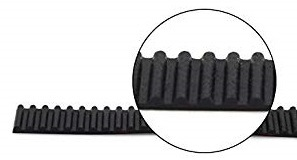
\includegraphics[max size={\textwidth}{\textheight}, scale=0.4]{Images/pulley.jpg}}
	\caption{Pulley belt \cite{merc}}
	\label{fig:belt}
\end{figure}

\subsection{Prototype Mounting Components}
Figure~\ref{fig:stand} shows a rough view of what the final prototype will look like when it is mounted on the mobile station. The specifics components for this prototype and how it was built are explained after it.

   \begin{figure}[H]
	\centering
	{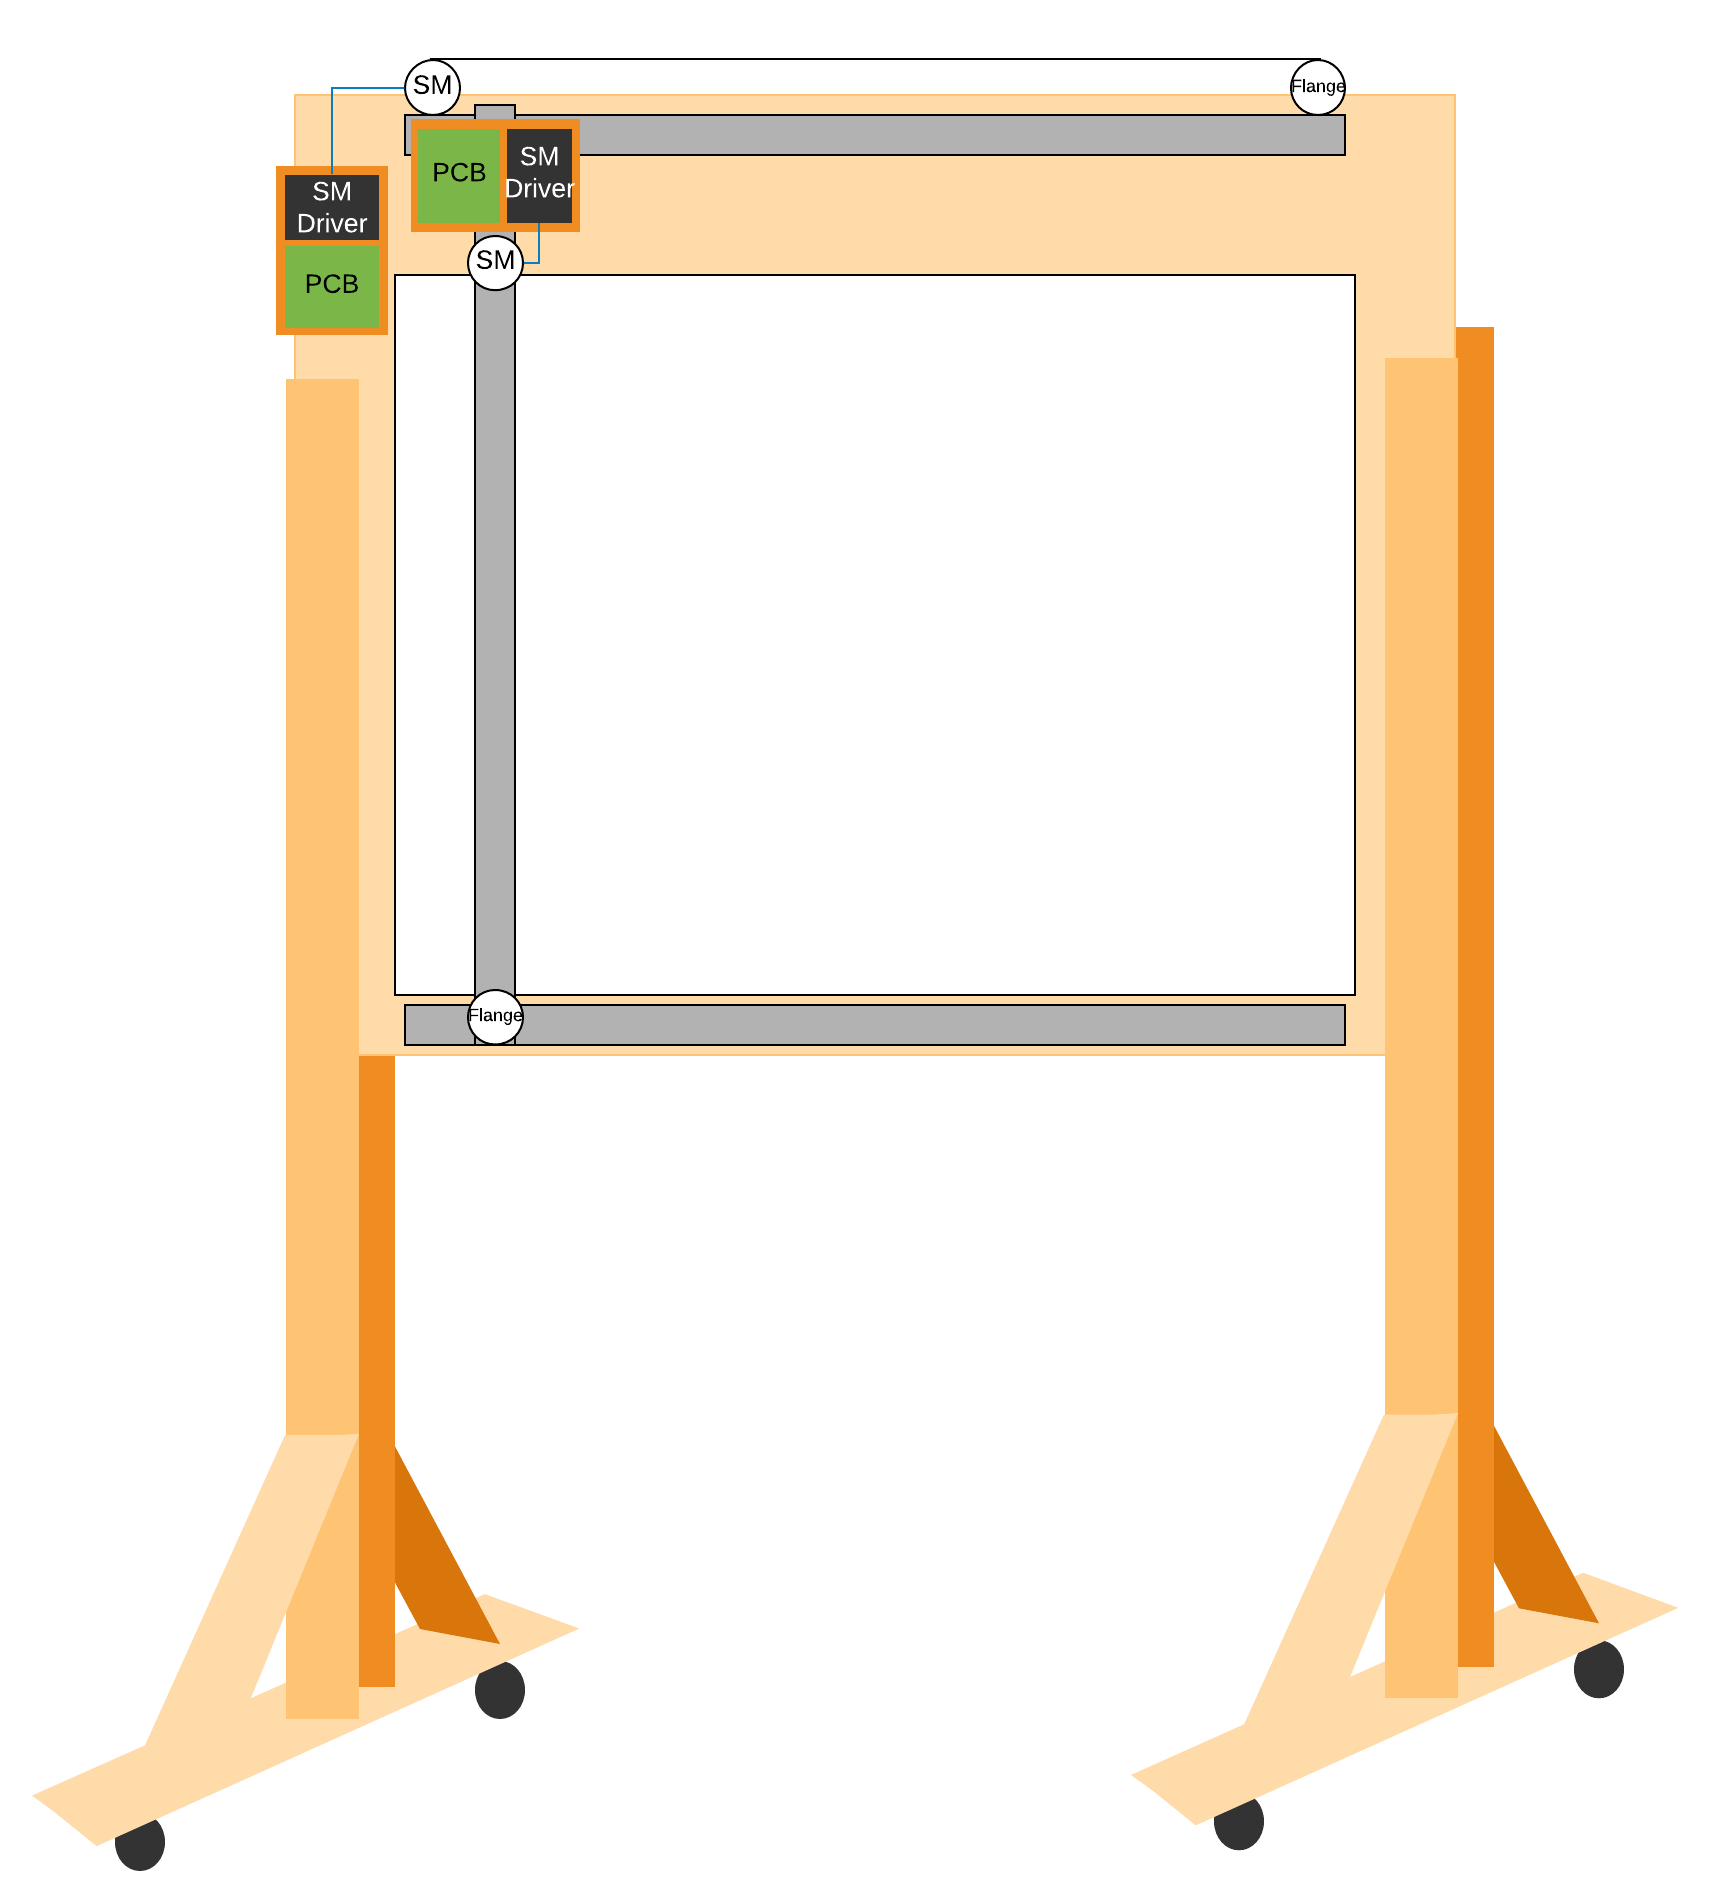
\includegraphics[max size={\textwidth}{\textheight}, scale=0.5]{Images/prot.png}}
	\caption{Rough image of the original concept for the prototype stand}
	\label{fig:stand}
\end{figure}

The main screws used were 3 inch T-25 star-headed screws. These were used to attach the horizontal tracks to the 2''x3'' posts, which were then attached to the plywood backing of the whiteboard. These screws were also used to mount the whiteboard to the wood backing. Two 2''x3'' posts were placed behind the tracks in order to give them more stability, as well as lift them off of the board enough to allow the tracks to travel in front of the whiteboard. Three more 2''x3'' posts were mounted on the back of the wooden backing as well so the plywood that the whiteboard is attached to would not bow or warp due to any changes in the environment. In order to stand the board, two 2''x4'' pieces of wood were placed at the bottom of the posts holding the stand up. Wheels were then attached to the bottom of this post to make the prototype stand mobile for Projects Day.\par
\setlength{\parindent}{2.5ex}
Washers and nuts were used to connect the pulley belt to the carriages on the x and y axes, which allow the eraser to move when the stepper motors rotate. Nuts and bolts were then used to connect the stepper motor system to the y axis. A metal L brace was used to mount the other flange to the opposite side of each axis from the stepper motors. Finally, braces were used to clamp the eraser to the carriage that moves across the Y axis.\par
\setlength{\parindent}{2.5ex}
The dimensions of the whiteboard prototype are shown in the next two figures. More information and details about how the system was created, built, and complete can be found in the \textit{Project Prototype} section of this report.

   \begin{figure}[H]
	\centering
	{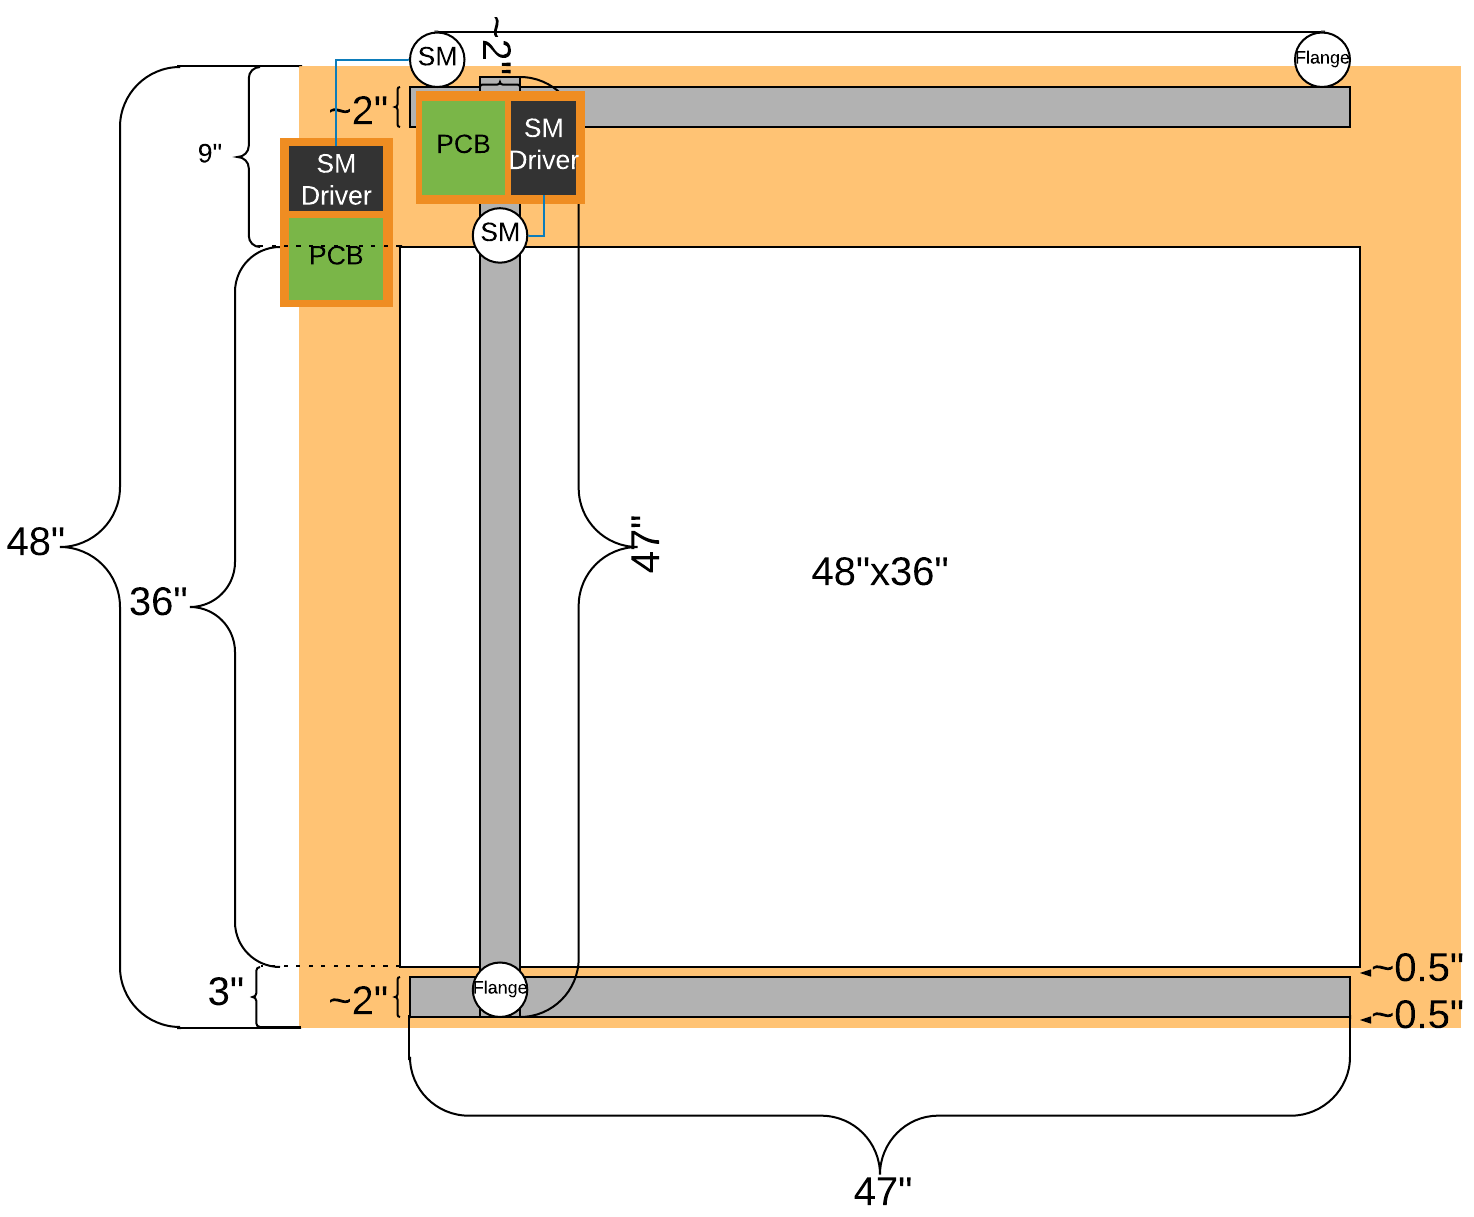
\includegraphics[max size={\textwidth}{\textheight}, scale=0.65]{Images/front_view.png}}
	\caption{Front view of the Smart Eraser system with dimensions}
	\label{fig:front_view}
\end{figure}   
\begin{figure}[H]
\centering
{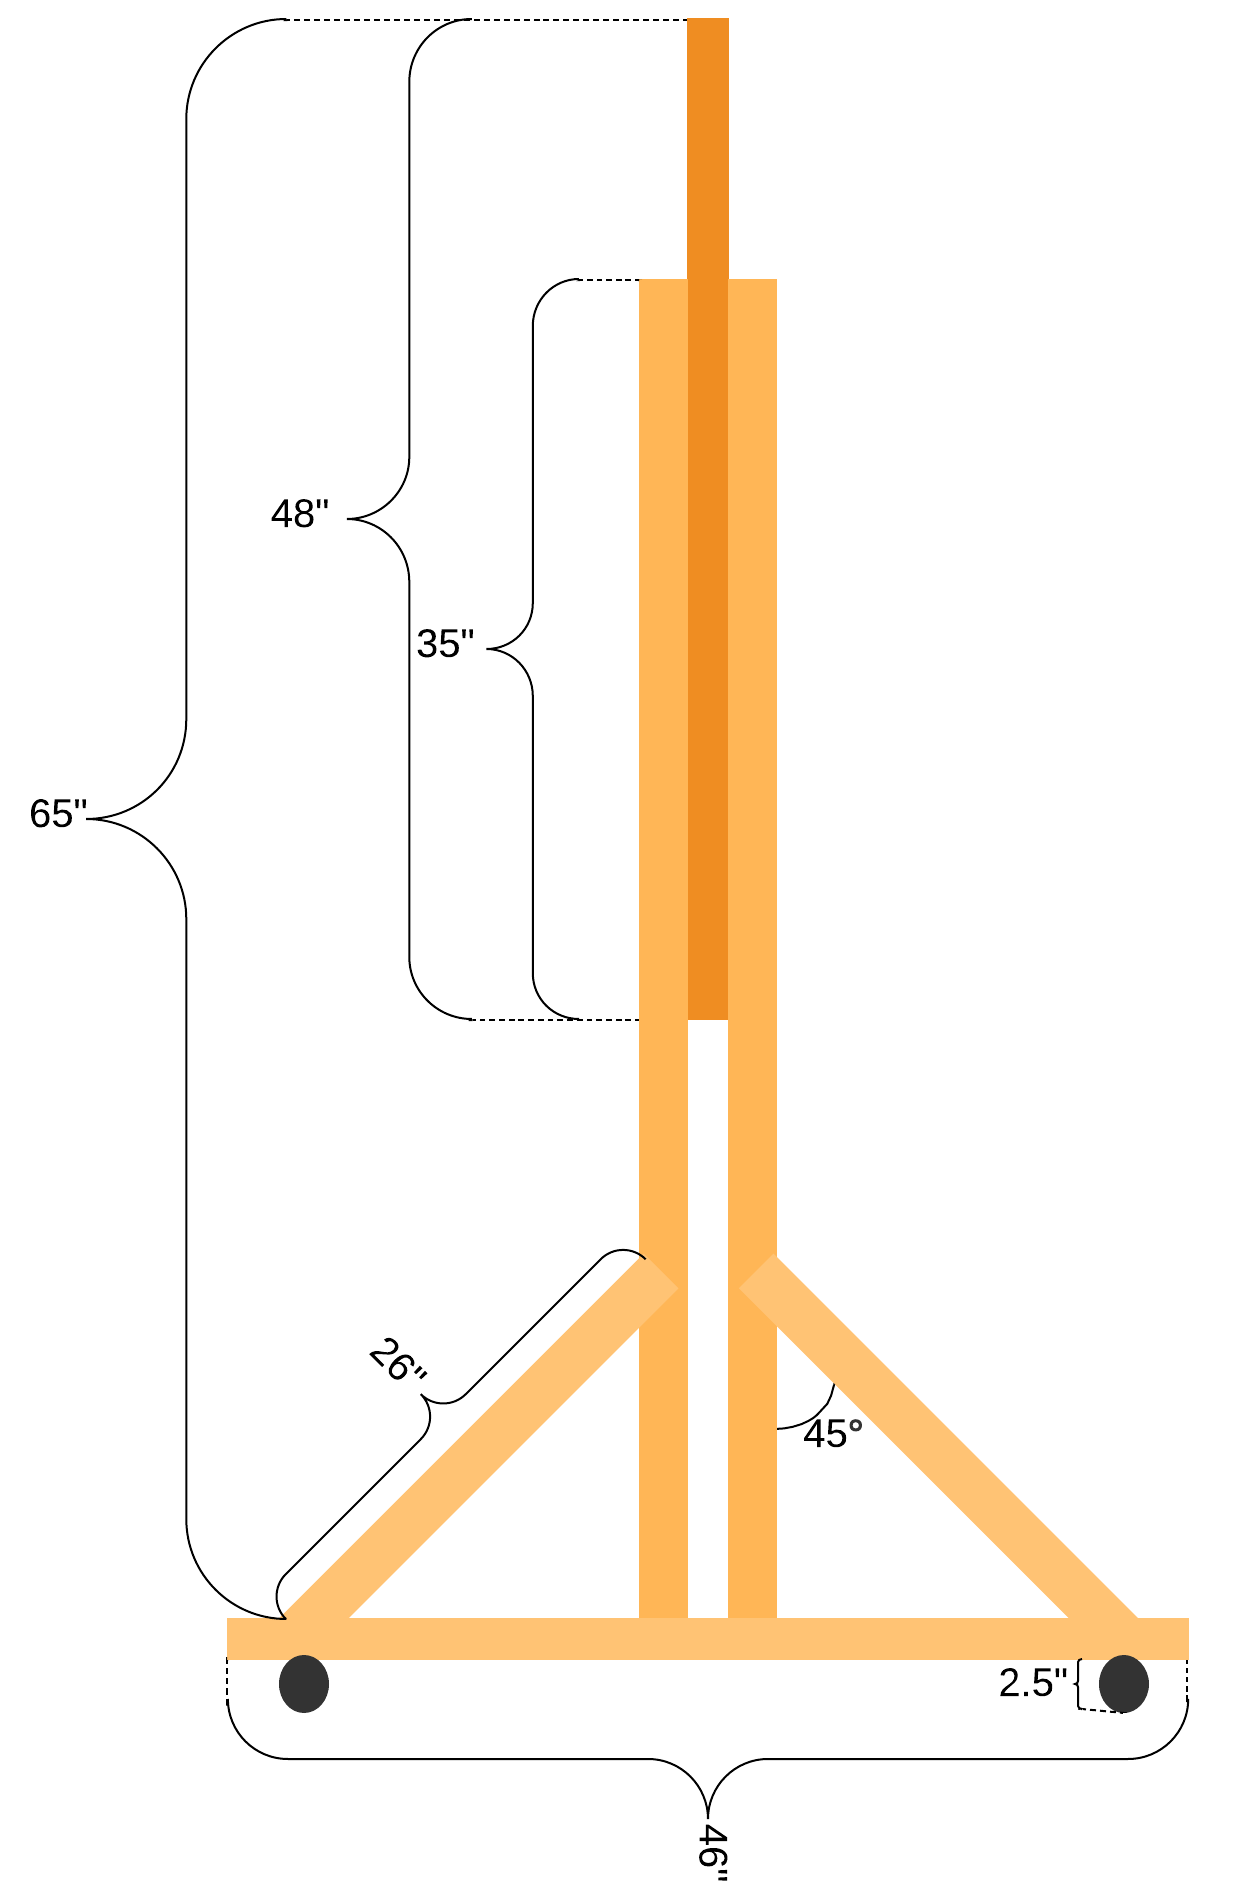
\includegraphics[max size={\textwidth}{\textheight}, scale=0.50]{Images/side_view.png}}
\caption{Side view of the Smart Eraser system with dimensions}
\label{fig:side_view}
\end{figure}

\subsection{Boundaries}

\setlength{\parindent}{2.5ex} Because of the problems encountered with the wireless communication via the Arduino and the Kuman wireless transceivers, the wireless communication system had to be completely redesigned using the HUZZAH32 Feather boards. This is a boundary, as this part had to be completely redone with Micropython, and the PCBs that were designed for the other system were not usable, and were abandonded in favor of mounting the systems separately on the whiteboard. \par
\setlength{\parindent}{2.5ex}
Unfortunately, configuration of the camera sensor proved to be a major obstacle. It involved writing a driver from scratch that needs to configure hundreds of different registers on the Arducam-5MP-Mini-Plus to output an RGB565 image. In order to show the system working, it was possible to take a picture with a phone and run it through software to convert it to the desired resolution and output format, and pre-load it onto the PSoC 6. It should be stated that the camera does work, and based off examples from the Arducam company, JPEG image data can be received from the camera. However, due to the complexity of JPEG image data and the fact that the image processing program written is for RGB565, there is nothing that can be done with this data in the scope of this project.

\subsection{Technical Advisor Backgrounds} \par	
\setlength{\parindent}{2.5ex} Dr. Hovannes Kulhandjian, who specializes in wireless communications and networking as well as digital signal processing. He has contributed advice and information pertaining to the wireless connectivity of the camera to the image processing microcontroller. Dr. Kulhandjian was the original mind behind the idea of this project as well. Because of this, he also contributed more specifications and features to implement in the project as its completion progressed.\par
\setlength{\parindent}{2.5ex}
Roger Moore has many specialties, ranging from tesla coil winding and electrical engineering to microcontroller usage, all stemming from his various research interests. He has contributed input on components that would likely lead to the most success in this project, as well as advice on how to perform the image processing.

\section{High-Level Risks}
The following list details the high-level risks of this project and what was done as a precaution against these risks in order to keep the development of the Smart Eraser safe.
\begin{itemize}
	\item Power system malfunction causing shorts:
		\begin{itemize}
		\item Ensure a secure connection of the power to the components from the batteries
		\item Have all wired connections complete before the power is applied
		\item If connections cannot be completed before power is applied, ensure that the pin will be going into the right port.
		\end{itemize}
	\item Moving parts attached to whiteboard:
		\begin{itemize}
		\item Always stand away from whiteboard when in motion
		\item Always notify those around when it is about to start moving
		\item Identify the failsafe wire to unplug in order to emergency shutdown the moving parts
		\item Have a proximity-sensor system that will detect and warn someone who is approaching the whiteboard at too close of a distance
		\end{itemize}
	\item Use of power tools to create prototype:
		\begin{itemize}
		\item Have an experienced advisor watching over the construction of the prototype stand
		\item Wear safety glasses and gloves when needed
		\item Work in a well ventilated area with plenty of room
		\end{itemize}
\end{itemize}

\section{Milestone Schedule}
Table~\ref{table:3}, Table~\ref{table:4}, and Table~\ref{table:5} show the milestone schedule for the Smart Eraser project over two semesters.
\setlength{\parindent}{5ex}
\begin{table} [H]	
	\normalsize
	\centering
	\begin{tabular}{|l|l|l|}
		\hline
		\multicolumn{1}{|c|}{\textbf{Member Assign.}} & \multicolumn{1}{|c|}{\textbf{Start-End Date}} & \multicolumn{1}{|c|}{\textbf{Description}} \\
		\hline
		All & 10/12-10/19/18 & Complete Smart Eraser Project Proposal to be\\
		& & submitted to DPS Telecom for review. \\
		\hline
		All & 10/12-10/19/18 & Finalize the specifics of the budget. \\
		\hline
		All & 10/15-10/19/18 & 
		Create the Project Charter rough draft to be turned in.\\
		\hline
		All & 10/16-10/26/18 & Draft a more detailed blueprint of the physical Smart \\
		& & Eraser deliverable. \\
		\hline
		All & 10/16-10/26/18 & 
		Revise the Project Description; complete for future\\
		& & reference. \\
		\hline
		All & 10/16-10/26/18 & 
		Draft the flowchart to show the logical relationships \\
		& & between all connected devices within the project.\\
		\hline
		All & 10/18-10/19/18 & 
		Complete bi-monthly update presentation for Senior \\
		& & Design class. \\
		\hline
		Juan C. & 10/26-11/10/18 & 
		Complete a block diagram detailing the specific \\
		& & connections between the devices within the project.\\
		\hline
		Heather L. & 10/26-11/15/18 & 
		Research wireless communication and protocols to be\\
		& & used. \\
		\hline
		Heather L. & 10/26-11/15/18 & 
		Research the camera and how it will send data over  \\
		& & WiFi connection.\\
		\hline
		All & 11/1-11/2/18 & 
		Complete bi-monthly update presentation for Senior \\
		& & Design class. \\
		\hline
		Heather L. \& Chris Q. & 11/1-11/21/18 & 
		Research the microcontroller to be used  (DE1\_SoC).\\
		\hline
		Chris Q. & 11/1-11/21/18 & 
		Research the image processing program and what  \\
		& & programming language to use.\\
		\hline
		Juan C. & 11/1-12/1/18 &
		Research the mechanical system and the power connection \\
		& & it requires. \\
		\hline
		
		All & 11/15-11/16/18 & Complete bi-monthly update presentation for Senior \\
		& & Design class. \\
		\hline
		Chris Q. & 11/15-11/25/18 & Test initial information found on image processing\\
		& & program. \\
		\hline
		Heather L. & 11/15-11/25/18 & Test the microcontroller after researching the ports needed \\
		& & for the project.\\
		\hline
		Heather L. & 11/20-12/1/18 & Research the coordinate system; converts pixels to stepper \\
		& & motor rotations in the mechanical system.\\
		\hline
		All & 11/29-11/30/18 & 
		Complete bi-monthly update presentation for Senior \\
		& & Design class. \\
		\hline
		All & 12/1-12/17/18 & 
		Complete the final draft of the Project Charter.\\
		\hline
		All & 12/13-12/14/18 & 
		Present Project Charter to Senior Design class, professor, \\
		& & and academic advisor.\\
		\hline
\end{tabular} 
\caption{Senior Design Semester 1 - Research Phase}
\label{table:3}
\end{table}

\begin{table} [H]	
	\normalsize
	\centering
	\begin{tabular}{|l|l|l|}
		\hline
		\multicolumn{1}{|c|}{\textbf{Assignee}} & \multicolumn{1}{|c|}{\textbf{Start-End Date}} & \multicolumn{1}{|c|}{\textbf{Description}} \\
		\hline
		All & 1/5/19 - 1/6/19 			& Finalize parts needed and decide what order to buy them for the \\
		& & project. \\
		\hline
		All & 1/6/19 - 1/9/19 			& Complete budget increase justification and send to Dr. Stillmaker. \\
		\hline
		Juan C. & 1/6/19-1/16/19	 	& Assist in research of how to get Linux onto DE1\_SoC Board; research the \\
				&						& micro SD card needed and the how to implement the QSYS system \\
				&						& to run with Linux. \\
		\hline
		Heather L. & 1/15/19 - 1/20/19 	& Figure out how stepper motors programmed with Arduino. \\
		\hline
		Chris Q. & 1/15/19 - 1/30/19 	& Research and implement Linux onto the DE1\_SoC. \\
		\hline
		Juan C. & 1/16/19 - 1/31/19 	& Create schematic for wooden frame of prototype stand. \\
		\hline
		Heather L. & 1/20/19 - 2/5/19 	& Figure out wireless communication with Arduino and wireless \\ 			&					& transceivers. \\
		\hline
		Chris Q. & 1/20/19 - 1/30/19 	& Develop system in QSYS that allows the HPS (Linux) to \\
				&						& communicate with its peripherals (FPGA components). \\
		\hline
		Chris Q. & 1/31/19 				& Decided to change microcontroller from DE1\_SoC to PSoC 6 under \\ 
				&						& advisement from Roger Moore. \\
		\hline
		Juan C. & 1/31/19 - 2/19/19 	& Develop more in-depth blueprint of wooden stand measurements and \\
				&						& dimensions. \\
				\hline
		Chris Q. & 2/2/19 - 2/7/19 		& Research PSoC 6 IDE Modus Toolbox. \\
		\hline
		Heather L. & 2/5/19 - 2/18/19 	& Combine stepper motor code with wireless communication for \\
				&						& wireless stepper motor system. \\
		\hline
		Chris Q. & 2/5/19 - 2/15/19 	& Create system within Modus Toolbox for PSoC 6 to connect to \\
				&						& needed peripherals. \\
		\hline
		Juan C. & 2/14/19 - 2/19/19 	& Determine all different types of screws, nuts, and bolts needed \\
				&						& for each individual part of the stand. \\
		\hline
		Chris Q. & 2/15/19 - 2/18/19 	& Research camera modules suitable for connection with the PSoC 6. \\
		\hline
		Heather L. & 2/18/19 - 3/11/19 	& Create and assemble PCBs with stepper motors, drivers, the \\ 
				&						& Arduino, and the power needed for all. \\
		\hline
		Chris Q. & 2/18/19 - 3/15/19 	& Develop SPI communication between the Arducam camera and the \\ 		&						& PSoC 6 microcontroller. \\
		\hline
		Juan C. & 2/20/19 - 3/15/19 	& Design mechanical system involving pulleys and linear motion \\
				&						& system. \\
		\hline
		Chris Q. & 2/25/19 - 3/2/19 	& Research image processing program in C with raw data. \\
		\hline
		Chris Q. & 3/2/19 - 3/9/19 		& Create program that translates a colored RGB565 image to \\
				&						& grayscale. \\
				\hline
		Heather L. & 3/4/19 - 3/13/19 	& Create algorithm to find outermost edges of markings on \\
				&						& whiteboard with Chris's processed image data. \\
		\hline
		All & 3/4/19 - 3/14/19 			& Prepare for Midterm Project Presentations. \\
		\hline
		Chris Q. & 3/9/19 - 3/16/19 	& Create program that detects edges in the converted grayscale \\ 		&						& image using sobel edge detection. \\
		\hline
		All & 3/14/19 - 4/12/19 		& Write rough draft of final project report. \\
		\hline
		Juan C. & 3/15/19 - 3/31/19 	& Assemble entire wooden prototype stand. \\
		\hline
		Chris Q. & 3/16/19 - 4/14/19 	& Continue trying to configure Arducam camera with PSoC 6. \\
		\hline
		Juan C. & 3/31/19 - 4/12/19 	& Mount all mechanical parts including tracks, pulley system, and \\
				&						& stepper motors to wooden stand. \\
		\hline
		Heather L. & 4/1/19 - 4/3/19 	& Wireless communication with Arduinos stopped working - come up \\  	&						& with alternative. \\
		\hline
	\end{tabular} 
\caption{Senior Design Semester 2 - Implementation Phase - Part 1}
\label{table:4}
\end{table}		
		
\begin{table} [H]	
	\normalsize
	\centering
	\begin{tabular}{|l|l|l|}
		\hline
		\multicolumn{1}{|c|}{\textbf{Assignee}} & \multicolumn{1}{|c|}{\textbf{Start-End Date}} & \multicolumn{1}{|c|}{\textbf{Description}} \\
		\hline			
		Juan C. & 4/12/19 - 4/15/19 	& Design power system to connect to stepper motors, their drivers, \\
		&						& and the HUZZAH32 boards on the system. \\
		\hline
		Heather L. & 4/14/19 - 4/16/19 	& Learn basics of Micropython for new microcontrollers. \\
				\hline
		Chris Q. & 4/14/19 - 4/17/19 	& Help Heather with learning Python language. \\
		\hline
		Heather L. & 4/14/19 - 4/17/19 	& Figure out code for stepper motors on new HUZZAH32 \\
					&					& microcontrollers. \\
		\hline
		Heather L. & 4/14/19 - 4/21/19 	& Create algorithm to move stepper motors in a serpentine-like way \\
					&					& to erase the markings using the outermost edges found in the \\
					&					& previously made algorithm. \\
		\hline
		Heather L. & 4/14/19 - 4/17/19 	& Create simple messaging program between two HUZZAH32s to test \\ 			&					& wireless communication. \\
		\hline
		All & 4/17/19 					& Create and finalize Projects Day poster. \\
		\hline
		Juan C.   & 4/15/19 - 4/21/19   & Create UART connection between HUZZAH32 and PSoC 6 to send \\
					&					& instructions for stepper motors. \\
		\hline
		Heather L. & 4/17/19 - 4/20/19 	& Combine wireless communication with stepper motor instructions \\
					&					& to create wireless stepper motor system. \\
		\hline
		Chris Q. & 4/17/19 - 4/28/19 	& Help Heather integrate stepper motor movement algorithms and \\
					&					& image processing program. \\
		\hline
		Juan C. & 4/17/19 - 4/26/19 	& Research motion detection system with ultrasonic sensor and \\
					&					& HUZZAH32 board. \\
		\hline
		Juan C. & 4/20/19 - 4/22/19 	& Test power system on breadboard and order necessary parts. \\
		\hline
		Heather L. & 4/20/19 - 4/22/19 	& Figure out angle of stepper motor rotations needed to move one \\
					&					& ``pixel'' length of the image taken of the whiteboard for \\
					&					& coordinates. \\
				\hline
		Juan C. & 4/22/19 				& Mount power system to wooden stand with HUZZAH32 boards and \\
					&					& stepper motor drivers. \\
		\hline
		Heather L. & 4/22/19 - 4/28/19 	& Combine standalone algorithms, written in C with a dummy matrix, \\
				&						& with the actual image data that will be processed in order to \\
				&						& give correct instructions to stepper motors for whiteboard. \\
		\hline
		All & 4/22/19 - 4/30/19 		& Think of Projects Day, what to talk about, and how to present to \\
				&						& the audience. \\
		\hline
		Juan C. & 4/25/19 - 4/27/19 	& Decide how to connect to system as a failsafe for someone \\
					&					& standing too close to moving parts. \\
		\hline
		Juan C. & 4/28/19 				& Mount ultrasonic sensor to prototype with indicator LEDs. \\
		\hline
		All & 5/2/19 - 5/9/19 			& Create Final Project report presentation and practice. \\
		\hline
		All & 4/30/19 - 5/9/19 			& Write final draft of Final Project report. \\
		\hline
		All & 5/7/19 					& Projects Day. \\
		\hline
		All & 5/9/19 					& Final Project report due. \\
		\hline
		All & 5/9/19 					& Final Project Presentation day. \\
		\hline
	\end{tabular} 
	\caption{Senior Design Semester 2 - Implementation Phase - Part 2}
	\label{table:5}
\end{table}

\section{Test Plan}

The Test Plan in Figure~\ref{fig:test1}, Figure~\ref{fig:test2}, Figure~\ref{fig:test3}, Figure~\ref{fig:test4}, and Figure~\ref{fig:test5} was made to test the features of the Smart Eraser as they are completed. The test plan includes what feature is being tested, who is in charge of creating that feature, and who is in charge of testing that feature. It then lists the success criteria, which is what determines if the test was a success, and the stopping criteria, which is what determines if a test needs to be stopped.

\begin{figure}[H]
	\centering
	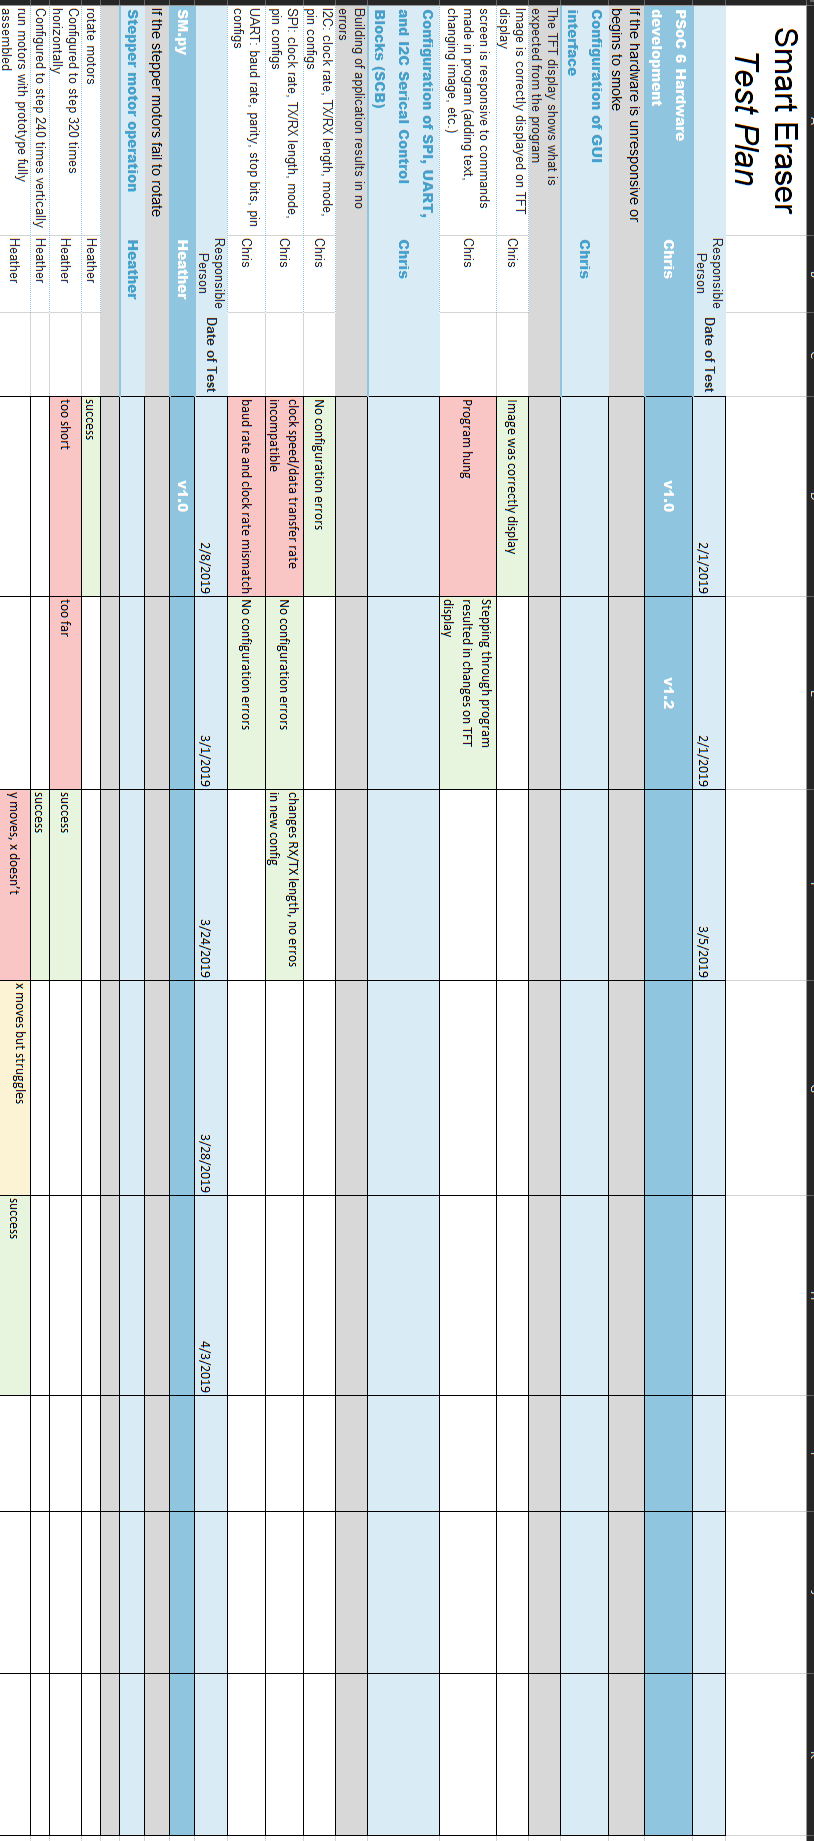
\includegraphics[max size={\textwidth}{\textheight}]{Images/testplan1V.png}
	\caption{Test Plan for the Smart Eraser - Part 1}
	\label{fig:test1}
\end{figure}

\begin{figure}[H]
	\centering
	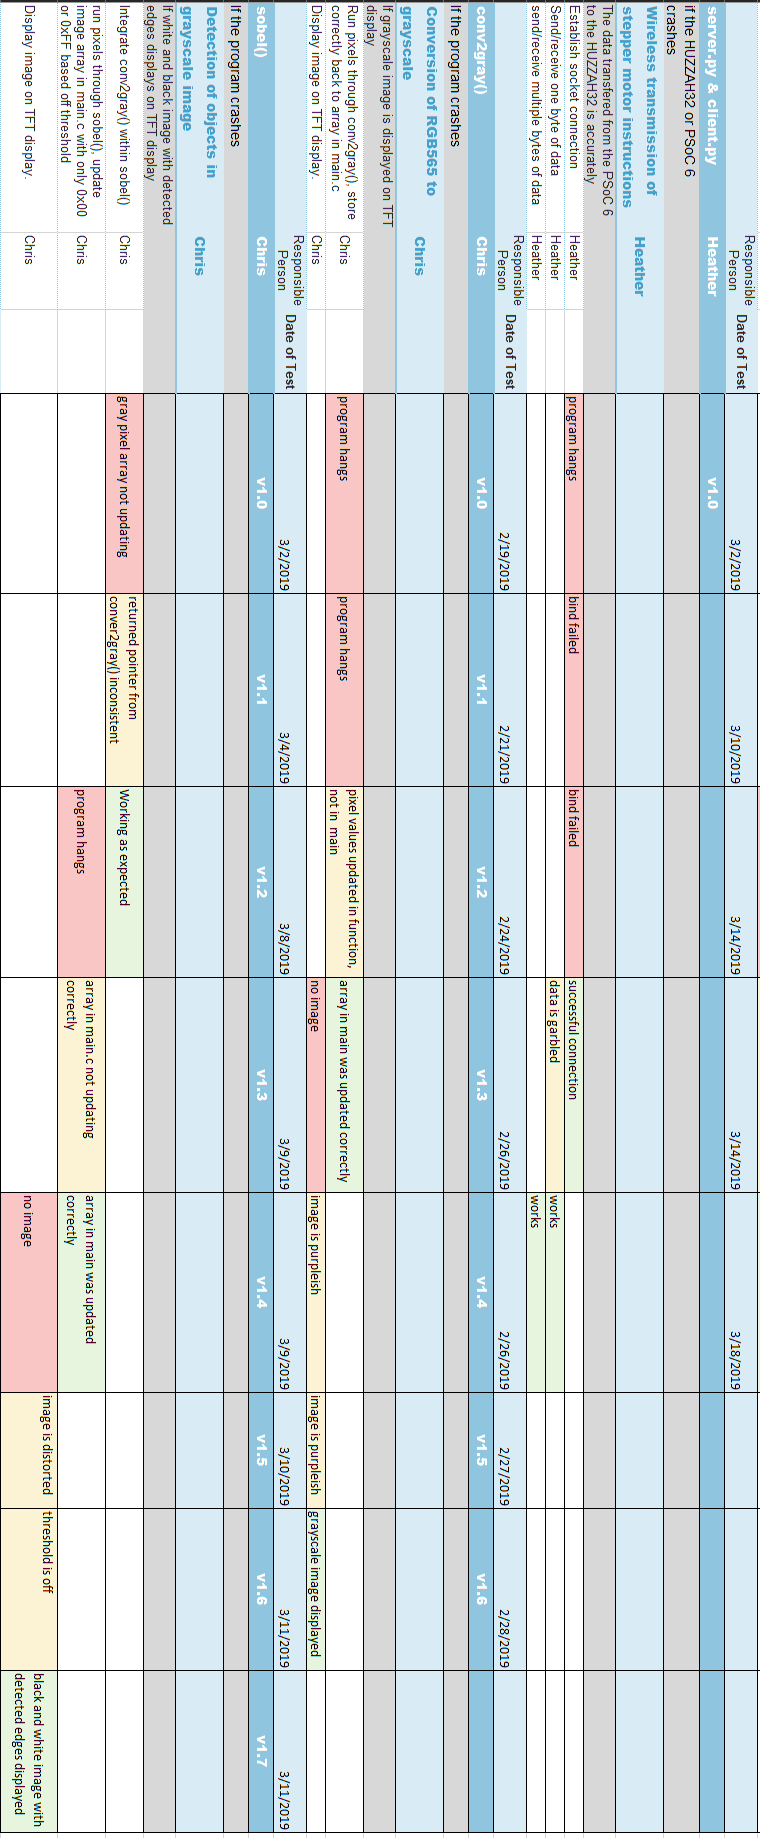
\includegraphics[max size={\textwidth}{\textheight}]{Images/testplan2V.png}
	\caption{Test Plan for the Smart Eraser - Part 2}
	\label{fig:test2}
\end{figure}

\begin{figure}[H]
	\centering
	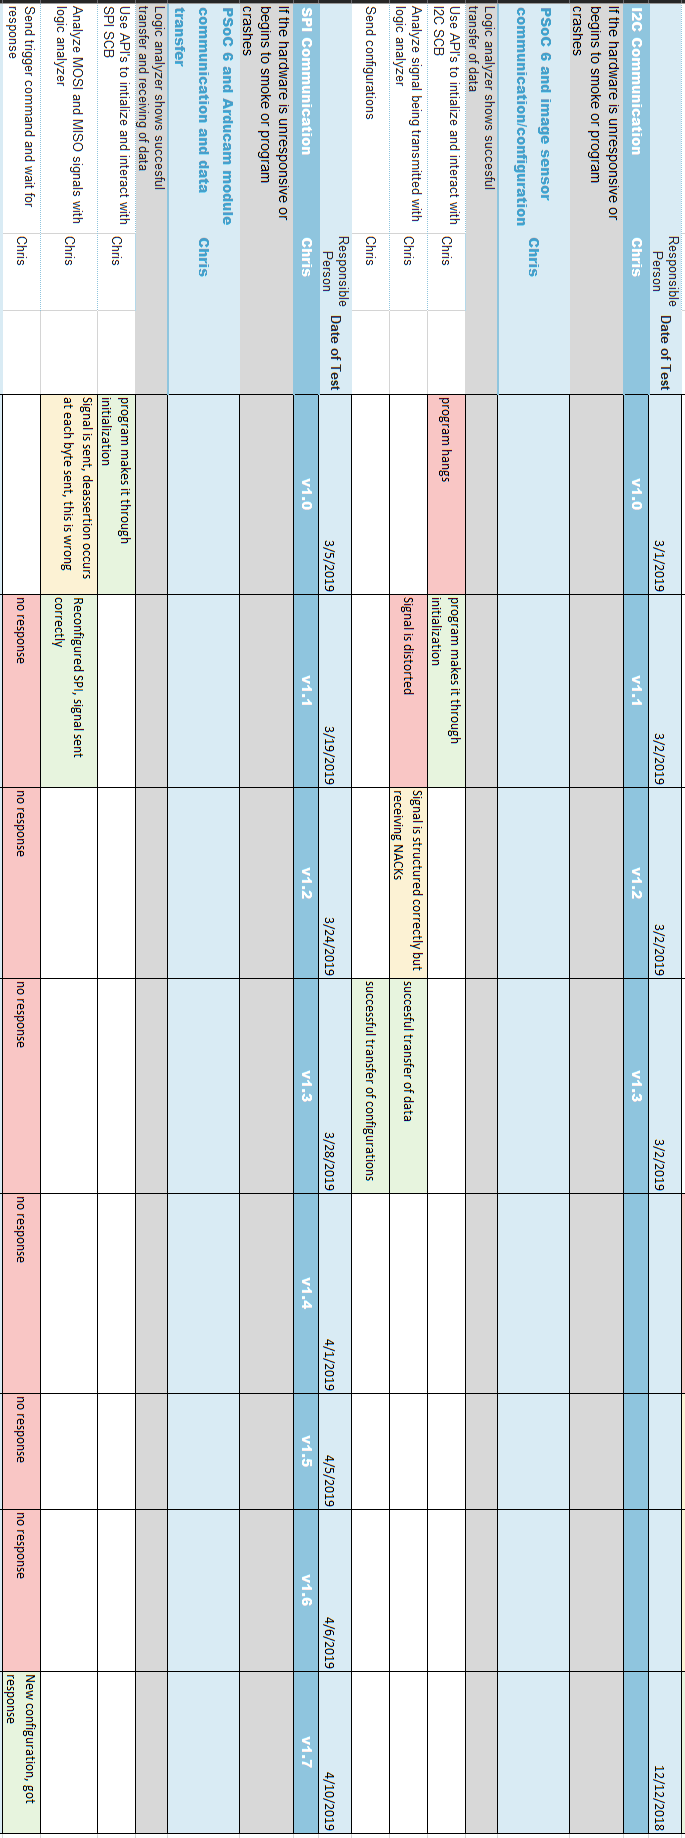
\includegraphics[max size={\textwidth}{\textheight}]{Images/testplan3V.png}
	\caption{Test Plan for the Smart Eraser - Part 3}
	\label{fig:test3}
\end{figure}

\begin{figure}[H]
	\centering
	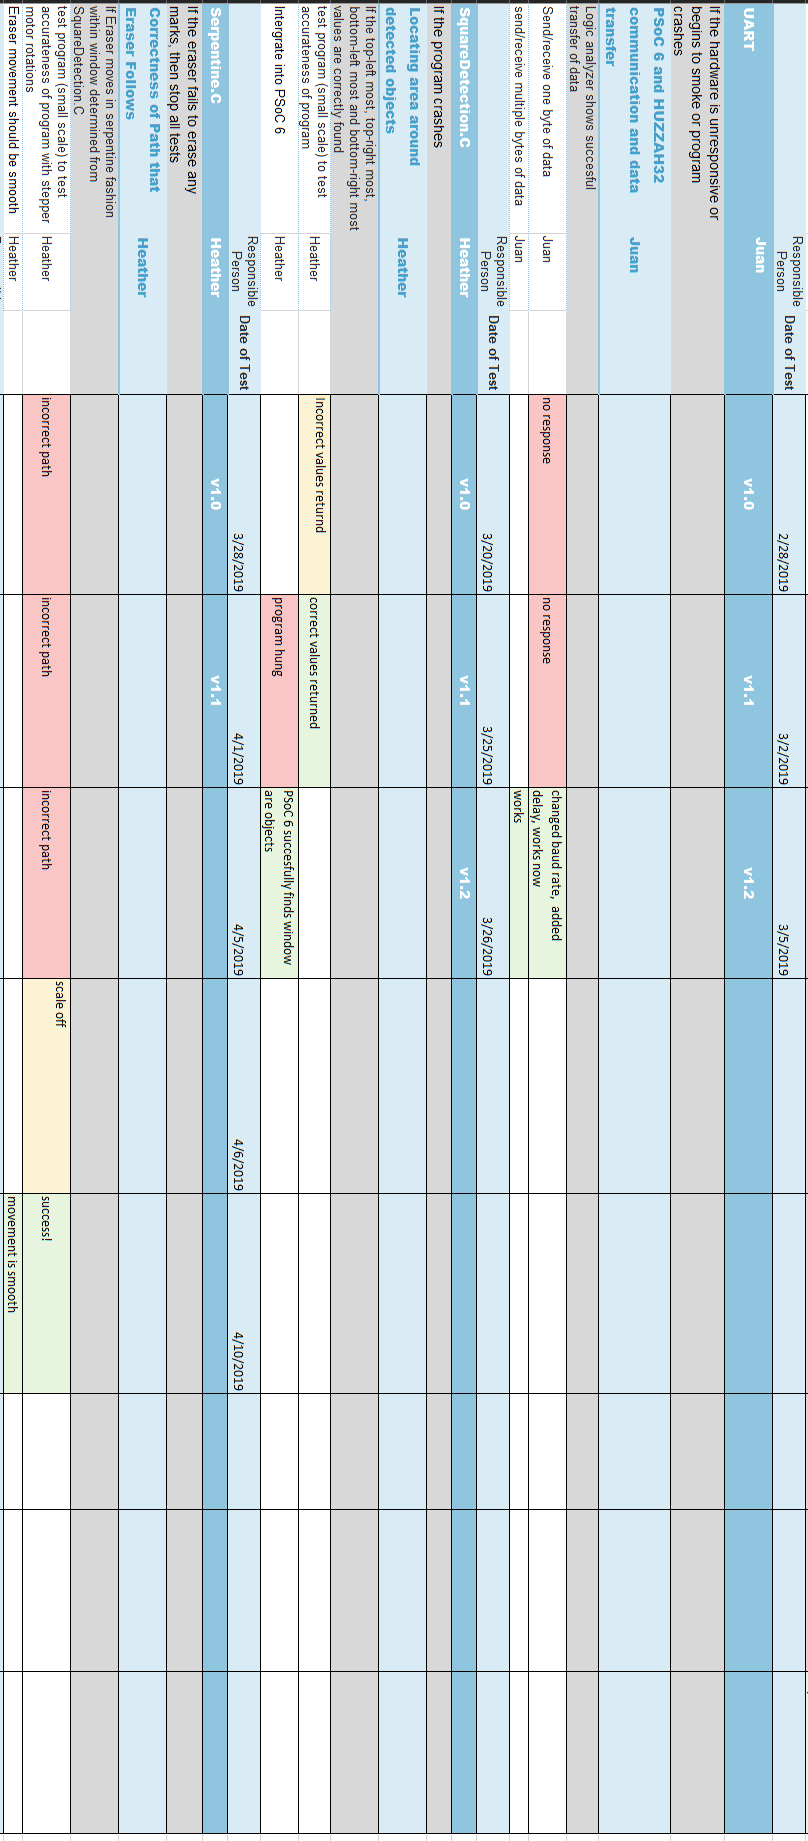
\includegraphics[max size={\textwidth}{\textheight}]{Images/testplan4V.png}
	\caption{Test Plan for the Smart Eraser - Part 4}
	\label{fig:test4}
\end{figure}

\begin{figure}[H]
	\centering
	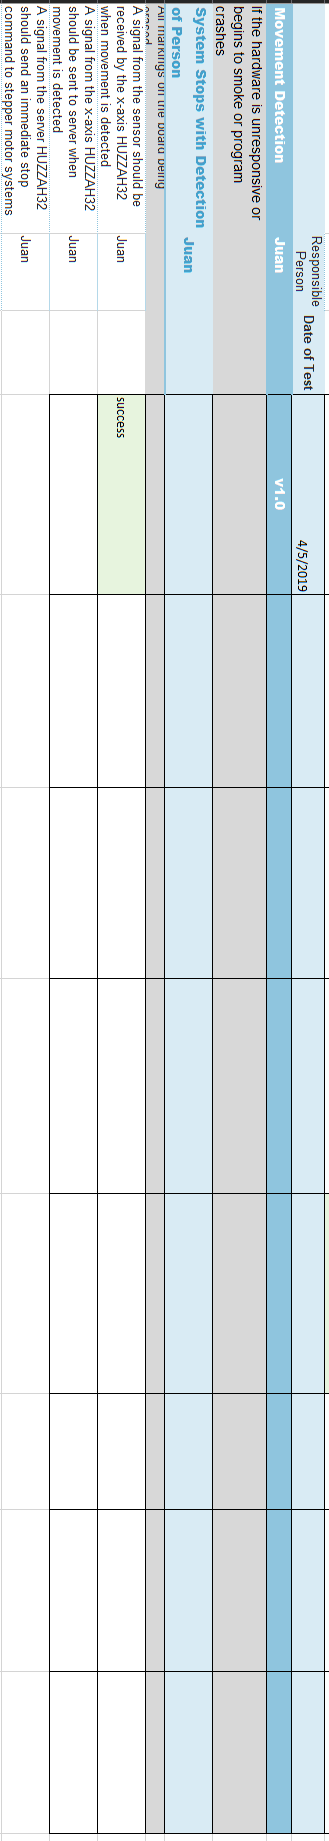
\includegraphics[max size={\textwidth}{\textheight}]{Images/testplan5V.png}
	\caption{Test Plan for the Smart Eraser - Part 5}
	\label{fig:test5}
\end{figure}

\section{Gantt Charts}

Figure~\ref{fig:GANTT186A} and Figure~\ref{fig:GANTT186B} show the GANTT chart schedules over the next two semesters. These list the tasks to be completed, who is in charge of what task, and the time duration the task is expected to take.

\begin{figure}[H]
	\centering
	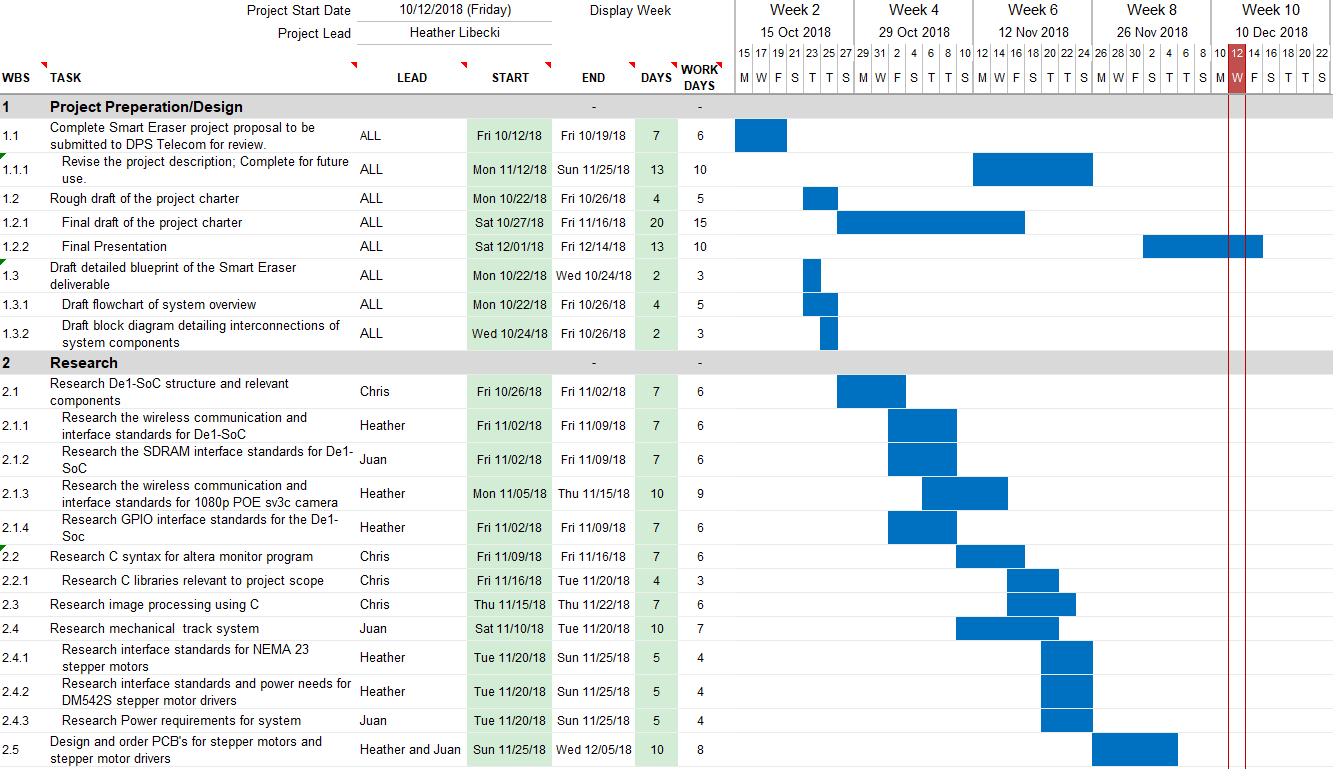
\includegraphics[max size={\textwidth}{\textheight}]{Images/GANTTchart186A.png}
	\caption{GANTT chart for Senior Design Semester 1 - Research Phase}
	\label{fig:GANTT186A}
\end{figure}

\begin{figure}[H]
	\centering
	{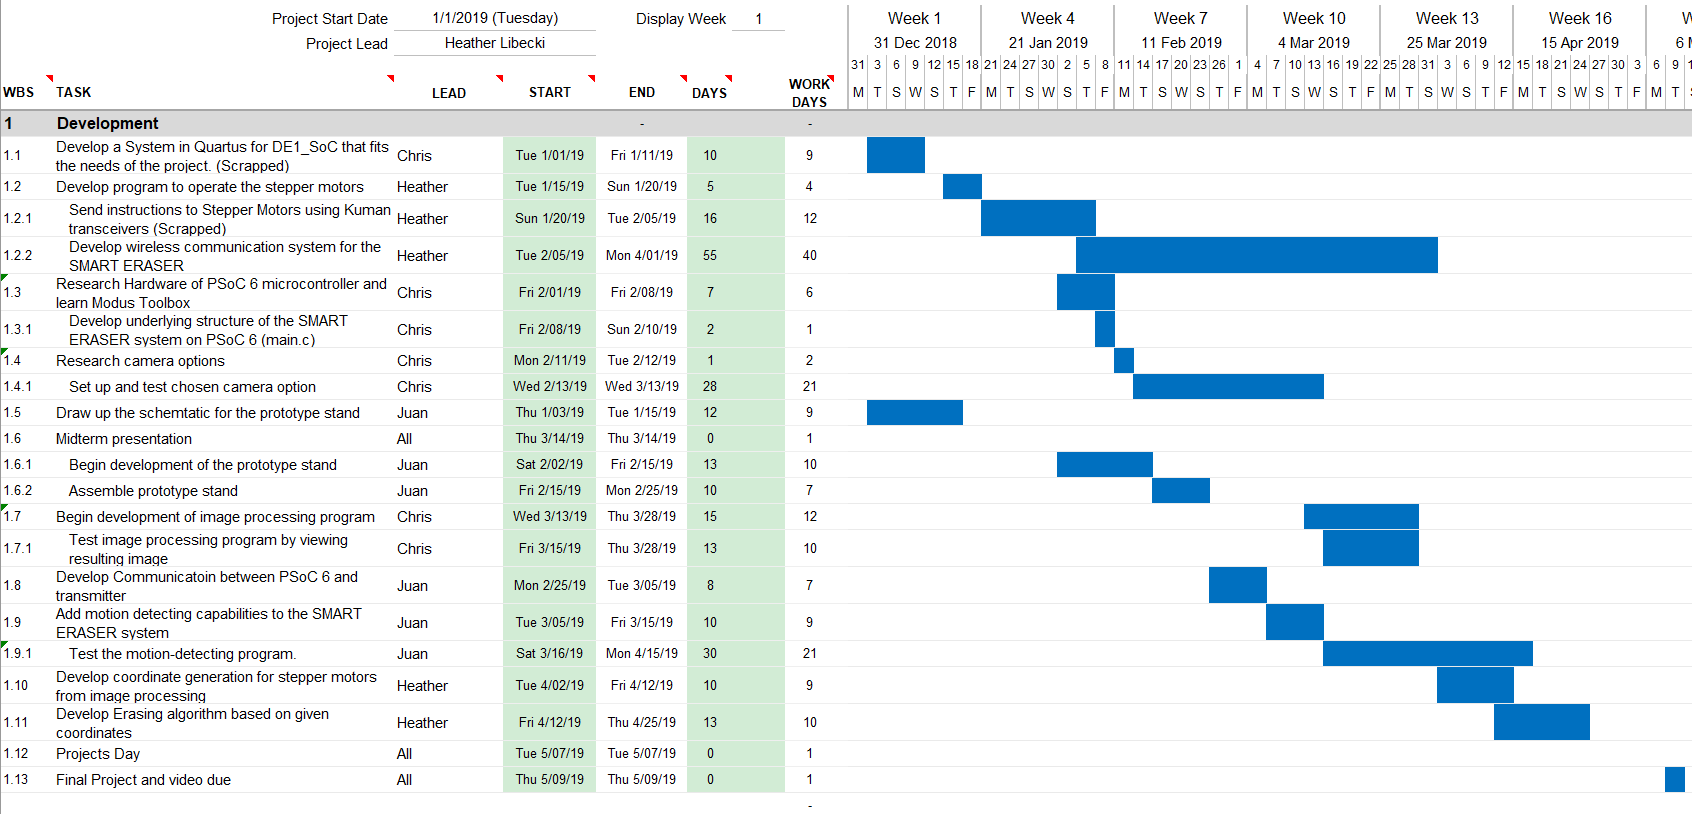
\includegraphics[max size={\textwidth}{\textheight}]{Images/GANTTchart186B.png}}
	\caption{GANTT chart for Senior Design Semester 2 - Implementation Phase}
	\label{fig:GANTT186B}
\end{figure}

\section{Equipment and Budget}
Table~\ref{table:1} lists the components that were bought in order to complete the Smart Eraser, as well as the company that made them and their cost. The costs are listed without taxes and shipping costs taken into account, but the total of the budget at the bottom of the table includes these. The components are listed in alphanumeric order.
\setlength{\parindent}{5ex}
\begin{table} [H]
	\normalsize
	\centering
	\begin{tabular}{|l|l|l|}
		\hline
		\multicolumn{1}{|c|}{\textbf{Component Name and Model}}  & 
		\multicolumn{1}{|c|}{\textbf{Production Company}}  & 
		\multicolumn{1}{|c|}{\textbf{Cost}} \\
		\hline
		\href{https://www.amazon.com/dp/B0728PDWY5/?coliid=I3K7SWFRMQ3A2F\&colid=22YAOKWOJAKA9\&psc=0\&ref_=lv_ov_lig_dp_it}{Aluminum GT2 40 Teeth 6.35mm Bore Timing Belt Pulley} 	& Uxcell 		& \$7.19 x4 \\
		\href{https://www.amazon.com/dp/B0728PDWY5/?coliid=I3K7SWFRMQ3A2F\&colid=22YAOKWOJAKA9\&psc=0\&ref_=lv_ov_lig_dp_it}{Flange} 	& 		& \\
		\hline
		\href{https://www.amazon.com/dp/B06VSYJ7HN/?coliid=I2N6U5HO8N5E5L\&colid=22YAOKWOJAKA9\&psc=0\&ref_=lv_ov_lig_dp_it}{Antenna Wireless Transceiver nRF24L01+PA+LNA} 	& Kuman 		& \$13.99 \\
		\hline
		\href{https://www.amazon.com/Arducam-Module-Camera-Arduino-Mega2560/dp/B013JUKZ48/ref=sr_1_fkmrnull_2_sspa?keywords=Arducam+Mini+Module+Camera+5+Megapixel+OV5647\&qid=1555715678\&s=gateway\&sr=8-2-fkmrnull-spons\&psc=1}{Arducam Mini Module Camera 5 Megapixel OV5647} 	& Arducam 		& \$39.99 \\
		\hline
		\href{https://store.arduino.cc/usa/arduino-mkr1000}{Arduino MKR1000 WiFi with Headers} 	& Arduino 		& \$33.95 \\
		\hline
		\href{https://www.adafruit.com/product/3619}{Assembled HUZZAH32-ESP32 Feather Board with Stacking} 	& Adafruit 		& \$21.95 x3 \\
		\href{https://www.adafruit.com/product/3619}{Headers} 	&  		&  \\
		\hline
		\href{https://www.amazon.com/dp/B06Y5VPSFN/?coliid=I1R941FDJ72L0R\&colid=22YAOKWOJAKA9\&psc=0\&ref_=lv_ov_lig_dp_it}{CNC Stepper Motor Driver DM542T} 	& STEPPERONLINE 		& \$38.99 x2 \\
		\hline
		\href{https://www.amazon.com/dp/B07GB3TSKH/?coliid=I3FJDEJ8MXP6RY\&colid=22YAOKWOJAKA9\&psc=0\&ref_=lv_ov_lig_dp_it}{Li-ion 9V Battery Charger Bay} 	& EBL Official 		& \$12.99 \\
		\hline
		\href{https://www.amazon.com/gp/product/B06XC9SMVN/ref=ppx_yo_dt_b_asin_title_o01_s00?ie=UTF8\&psc=1}{Magnetic Whiteboard 48''x36''} 	& Lockways 		& \$49.99 \\
		\hline
		\href{https://www.omc-stepperonline.com/nema-23-stepper-motor/nema-23-bipolar-18deg-126nm-1784ozin-28a-25v-57x57x56mm-4-wires-23hs22-2804s.html}{NEMA 23 CNC Stepper Motors} 	& STEPPERONLINE 		& \$19.99 x2 \\
		\hline
		\href{https://www.amazon.com/gp/product/B07JGTHVVL/ref=ppx_yo_dt_b_asin_title_o03_s00?ie=UTF8\&psc=1}{NEMA 23 Stepper Motor Mounting Bracket 4 pack} 	& Jiuwu 		& \$18.99 \\
		\hline
		\href{https://www.cypress.com/documentation/development-kitsboards/psoc-6-wifi-bt-pioneer-kit-cy8ckit-062-wifi-bt}{PSoC 6 WiFi-BT Pioneer Kit} 	& Cypress 		& \$99.00 \\
		\hline
		\href{https://www.pcbway.com/}{Stepper Motor PCBs} 	& PCBWay 		& \$147.00 \\
		\hline
		\href{https://www.homedepot.com/}{Various Braces and Glue} 	& Home Depot 		& \$27.46 \\
		\hline
		\href{https://www.homedepot.com/}{Various Screws, Nuts, and Bolts} 	& Home Depot 		& \$24.64 \\
		\hline
		\href{https://www.homedepot.com/}{Wood Plywood Backing 96''x48''} 	& Home Depot 		& \$39.82 \\
		\hline
		\href{https://www.homedepot.com/}{Wood 2''x4''} 	& Home Depot 		& \$12.27 x4 \\
		\hline
		\href{https://www.amazon.com/gp/product/B0748CNTFR/ref=ppx_yo_dt_b_asin_title_o05_s00?ie=UTF8\&psc=1}{10 Meter GT2 6mm Steel Core White Open Ended Timing} 	& Nineone 		& \$15.89 \\
		\href{https://www.amazon.com/gp/product/B0748CNTFR/ref=ppx_yo_dt_b_asin_title_o05_s00?ie=UTF8\&psc=1}{Belt} 	& 		&  \\
		\hline
		\href{https://www.accuride.com/ss0115-cassrc-carriage-for-115rc}{115RC Cassette with Stainless Steel Bearings} 	& Accuride 		& \$45.00 x3 \\
		\hline
		\href{https://www.accuride.com/al0115-0120rc-aluminum-track-without-pre-drilled-holes}{115RC 47'' Aluminum Track} 	& Accuride 		& \$36.22 x3 \\
		\hline
		\href{https://www.homedepot.com/}{2'' Caster Rubber Wheels with Swivel and Brake} 	& Home Depot 		& \$3.98 x4 \\
		\hline
		\href{https://www.amazon.com/gp/product/B0779ZSNS3/ref=ppx_yo_dt_b_asin_title_o01_s00?ie=UTF8\&psc=1}{9V Battery Clips} 	& BBTO US 		& \$6.25 \\
		\hline
		\href{https://www.mouser.com/ProductDetail/Keystone-Electronics/1294?qs=sGAEpiMZZMsb53hqUvtGaal96fsGiPnZeBRTs87TntQ\%3D}{9V Battery Holders for PCBs} 	& Mouser 		& \$1.90 x10 \\
		\hline
		\href{https://www.amazon.com/gp/product/B00GLK1BO2/ref=ppx_yo_dt_b_asin_title_o01_s01?ie=UTF8\&th=1}{9V Rechargeable Batteries 6 pack} 	& EBL Official 		& \$25.99 x2 \\
		\hline

		\hline
				\textbf{TOTAL COST} & & \ \textbf{\$1,202.13} \\
				\hline
				\textbf{Allotted Budget} & & \ \textbf{\$930.00} \\
				\hline
				\hline
				\textbf{Over Budget Cost} & & \ \textbf{\$272.13} \\
		\hline 
	\end{tabular} 
	\caption{Cost of components for project}
	\label{table:1}
\end{table}	

As shown in the table for the budget, this project has exceeded the original expected budget by almost \$300. The original estimate was not taking into account the problems that were run into during the course of the project's life cycle. For example, the Arduino and Kuman wireless transceivers had to be changed to the HUZZAH32 Feather boards for the wireless communications because of their inoperability. This and a few other unforeseen circumstances pushed the budget over the limit. Now that this experience has been had, for future projects, more research will be done on what exactly will be needed for each step of the way, and which approach will be the best before confirming the budget. This way, perhaps the budget can be more closely followed.\par

\setlength{\parindent}{2.5ex}Along with the components listed in the budget, the resources in Table~\ref{table:2} were also used to complete the project.

\begin{table} [H]
	\normalsize
	\centering
	\begin{tabular}{|l|l|l|}
		\hline
		\multicolumn{1}{|c|}{\textbf{Name of Equipment}}  & 
		\multicolumn{1}{|c|}{\textbf{Type}}  & 
		\multicolumn{1}{|c|}{\textbf{Description}} \\
		\hline
				DipTrace 	&  Software		& Designing PCBs \\
		\hline
				Arduino IDE 	&  Software		& For programming and running the Arduinos when \\
								&  				& they were being used for the wireless \\
								&  				& communications. \\
	    \hline
				Lucid Charts 	&  Software		& For all figures, flowcharts, and diagrams \\
								&  				& that were created \\
		\hline
				Modus ToolBox IDE 	&  Software		& Programming and setting up the system for the \\
									&  				& PSoC 6. \\
		\hline
				uPyCraft IDE 	&  Software		& Programming the HUZZAH32 Feather Boards. \\
		\hline
				Various connectors and jumper cables	&  Hardware		& For connections between components  \\
		\hline
				Digital Multimeter 	&  Hardware		& For testing and recording voltages, currents, and \\
									&  				& resistances across components. \\
		\hline
				Solderless Breadboard 	&  Hardware		& For testing purposes. \\
		\hline
				Logic Analyzer 	&  Hardware		& For testing purposes. \\

		\hline 
	\end{tabular} 
	\caption{Equipment used besides the components bought}
	\label{table:2}
\end{table}	

\section{Roles of Team Members}
This section contains a more in depth look at what the specific roles of each team member were throughout this project. Included in this section is each member's areas of expertise, areas they were not experienced in, and what they had to work on the most throughout the completion of the Smart Eraser.
\subsection{Heather Libecki}
She had the responsibility of being the project manager for the Smart Eraser project. She also wanted to take charge of the stepper motors and their operations. She has had previous experience with stepper motors and how they work, so she was ready to take on this task. The technical advisor Dr. Kulhandjian wanted the project to be as wireless as possible, so wireless transceivers were decided upon to communicate with the stepper motors from a master controller that would send instructions. She decided to take on the task of creating the wireless communications as well, as she has a personal interest in wireless connections and networking programming. Although she had no experience in wireless communications, she wanted to learn this for the project. Finally, because she was in charge of the connections and movement of the stepper motors, she needed to create the algorithms that would actually allow the stepper motors to move the eraser to where they needed to go based on the image processing that Chris did. She was responsible for the algorithm that would find the outer-most edges of the markings on the whiteboard, then for the algorithm that took those coordinates and created a serpentine-like path, out of stepper motor instructions, that the eraser would need to follow. The following list details her strengths and weaknesses that would assist her for this project.
\begin{itemize}
	\item Strengths: programming (Verilog, C programming), PCB design, mathematics, debugging, circuit implementation, problem solving, technical writing, public speaking
	\item Weaknesses: circuitry design, power systems, socket programming with Micropython 
\end{itemize} 
 \subsection{Chris Quesada}
Has experience in working with embedded systems and developing code for different applications. This project will be heavy on the software side, using both \textit{C} and \textit{Python} to receive data, analyze it, and then send an output.  He also developed the UART, SPI, and I\textsuperscript{2}C communications needed for the Smart Eraser system. A solid understanding  of arrays, pointers, and how information is stored in memory was applied towards implementing the  image processing techniques used to find pixels that represent markings in the digital image. His work in ECE 70, concepts and experience gained in CSCI 41, and research into image processing allowed for the succesful completion of the Smart Eraser  image processing capabilities. Researching SPI and I\textsuperscript{2}C in Embedded systems along with further research into theses communications along with UART during the Smart Eraser developement led to successful implementations of all three. He also assisted Heather with the developement of the wireless communicaions between the HUZZAH32 microcontrollers.
\begin{itemize}
	\item Strengths: programming (C, C++, Python),  programming concepts (arrays, pointers, structures, data types), embedded systems, developing algorithms, communications(SPI, UART, I\textsuperscript{2}C)
	
	\item Weaknesses: circuitry design, mathematics, public speaking, power
\end{itemize} \par
 \subsection{Juan Colin}
  Has experience in working with electrical systems and physical circuit design. He is proficient in the use of problem solving techniques to create a functioning system with given design specifications. His part of the project was dependent on learning the physical mechanical aspects of the design, and how the connected parts will be powered. Therefore, he was in charge of the main mechanical system as well as the wooden prototype stand, and how the power can be supplied to the technological components in order to allow all parts of the system to work properly and move the way they need to. He also used knowledge from previous classes to program a microcontroller to detect the presence of a person in front of the whiteboard in order to provide a safety measure because there are moving parts in this project. He needed to research Micropython from scratch and use that knowledge to accomplish this.
  
	\begin{itemize}
	\item Strengths: electrical systems, circuitry design, problem solving, power systems, public relations
	\item Weaknesses: programming (Assembly, Verilog), technical writing and spelling
\end{itemize}

\lstset{frame=tb,
	language=c,
	aboveskip=3mm,
	belowskip=3mm,
	showstringspaces=false,
	columns=flexible,
	basicstyle={\small\ttfamily},
	numbers=none,
	numberstyle=\tiny\color{gray},
	keywordstyle=\color{blue},
	commentstyle=\color{dkgreen},
	stringstyle=\color{mauve},
	breaklines=true,
	breakatwhitespace=true,
	tabsize=3
}

\section{Analysis and Design}

In this section, the implementation of the components that came together to make the Smart Eraser functional will be described.

\subsection{I\textsuperscript{2}C Communication - PSoC 6 to Arducam}
Inter-Integrated-Circuit(I\textsuperscript{2}C) is a popular method for interactions between processors and slower ICs. For optimal efficiency, short distances should be used so it is mainly for intra-board connections. The naming scheme used to define the components is referred to as a master/slave relationship where there is one master and one or more slaves. Communication between the master and slave is through messages, with the messages being structured in a specific way. A start and stop bit are used to indicate the start and end of a message. After the start bit, an address is given, usually 7-10 bits, followed by the read/write bit. As was the case with Arducam, the data sheets for slave devices often incorrectly list the slave address with the read/write bit included. Using the PSoC 6 APIs for the I\textsuperscript{2}C Serial Control Block(SCB) added a start and stop bit to the given slave address based on whether it was a read or write. So, after omitting the LSB of the slave address provided from Arducam, communications worked perfectly(0x78 - LSB = 0x3C). This is known as the address frame. There are also 2 data frames that ensue, each a byte wide. Between each frame either an ACK is received from the slave or the communication failed and the ACK bit is set to NACK. The flow of how a message is sent can be seen in Figure~\ref{fig:I2Cmessage}.

 \begin{figure}[H]
	\centering
	{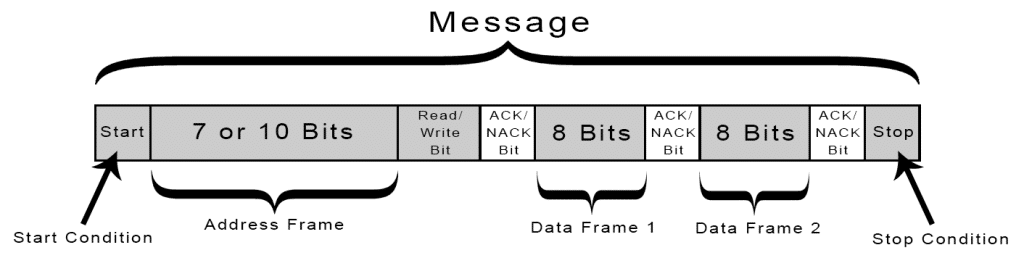
\includegraphics[max size={\textwidth}{\textheight}, scale=1]{Images/I2Cmessage.png}}
	\caption{Simple overview of an I2C message \cite{I2C}}
	\label{fig:I2Cmessage}
\end{figure}

Some confusion may arise when it is stated that in order to communicate with the Arducam module both I\textsuperscript{2}C and SPI are needed to do so. This is because the Arducam is just that, a module, that has different components. The difference between these two types of communication is that I\textsuperscript{2}C is needed to initialize the image sensor on the module, determining what is transferred to the FIFO storage, located on the module as well. For example, with I\textsuperscript{2}C, the resolution, format, and size of the image can be configured. With SPI, the actual capture and transfer of the image data from that FIFO storage is done. Basically, the I\textsuperscript{2}C can only interact with the image sensor itself and the SPI communication is for operating the entire module. The layout of the different components is shown in Figure~\ref{fig:ArducamBlock}\par
\setlength{\parindent}{2.5ex}

 \begin{figure}[H]
	\centering
	{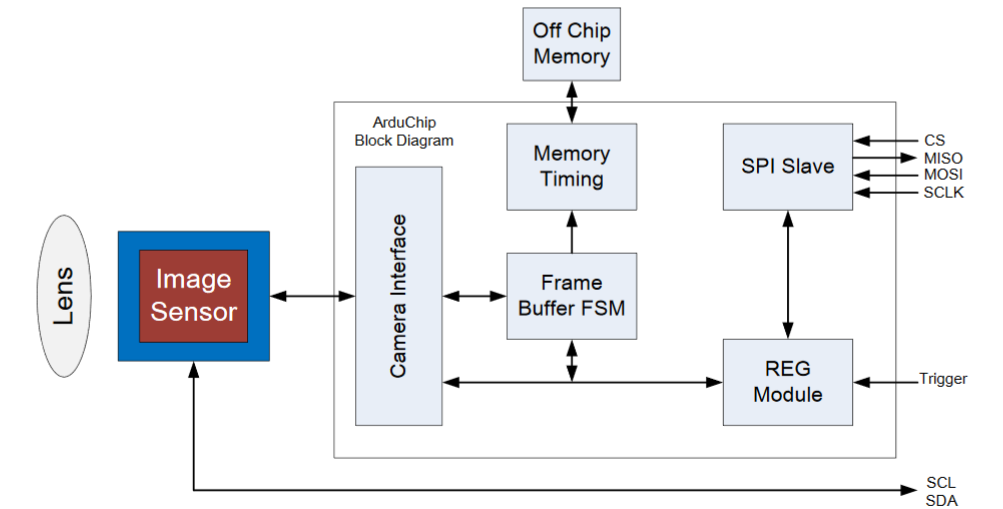
\includegraphics[max size={\textwidth}{\textheight}, scale=1]{Images/ArducamBlock.png}}
	\caption{Arducam module block diagram \cite{arducam}}
	\label{fig:ArducamBlock}
\end{figure}

Unfortunately due to time constraints, although the I\textsuperscript{2}C communication works correctly, attempts at configuring the image sensor to output RGB565 with a resolution of 320x240 were unsuccessful. This is due to the hundreds of control registers that can be found in the sensor and not knowing which ones need to be set and what values to set in them. This can be a project all on its own. However, the analysis and design will still be explained.\par
\setlength{\parindent}{2.5ex} 
In the file Arducam.C, found in ~\ref{A8}, MyCam\_Init() uses the Write\_I2C() function to send configuration signals to the image sensor of the Arducam module. These configurations are stored in structures in the beginning of the code file. As can be seen, just in the first configuration structure alone, there are over 250 configurations that need to be sent to the image sensor to get a RAW 1280x960 image stored to the FIFO buffer of the Arducam module. This is followed by another, much smaller set of configurations that is meant to resize the image. Due to the inability to set the output to RGB565, an attempt to receive RAW data was attempted and is the reasoning for sending theses configurations. Receiving RAW data requires another component to be added to the image processing, demosaicing, and is currently still in development. The Write\_I2C() function uses a combination of APIs provided by Cypress in order to interact with Serial Control Block 3 (SCB3) configured to be a I\textsuperscript{2}C master. It can be found in the section ~\ref{A6}.

 \begin{figure}[H]
	\centering
	{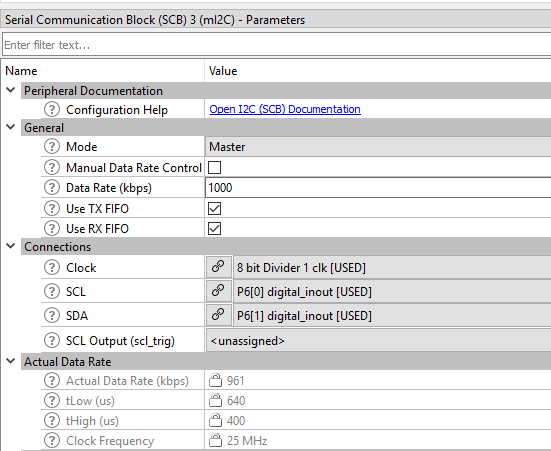
\includegraphics[max size={\textwidth}{\textheight}, scale=1]{Images/I2Chardware.png}}
	\caption{Hardware Configuration of I2C}
	\label{fig:I2Chardware}
\end{figure}



\subsection{SPI communication - PSoC 6 to Arducam}
Serial Peripheral Communication (SPI) is a common form of wired communication between different systems. The master/slave relationship used in I\textsuperscript{2}C is also used in SPI. There is no official standard for SPI however it is so widely used that it can be referred to as a De facto standard due to everyone operating along the same assumptions. These assumptions include the 4 modes SPI operate in and each mode is a different combination of the clock phase, when data is evaluated, and clock polarity, whether the clock is high or low when not in use. Once the mode has been decided, the slave clock dictates the rate of transaction between master and slave and therefore, the master must be configured accordingly. A Master-Out-Slave-In (MOSI) line feeds data, either MSB or LSB first, to the shift register in the SPI interface of the slave device. For every bit received, the slave will send a bit back to the master along the Master-In-Slave-Out (MISO) line. During a SPI exchange, every bit sent is a bit received and depending if you want to read or write data, the bits received are sometimes irrelevant (writing to slave).  

 \begin{figure}[H]
	\centering
	{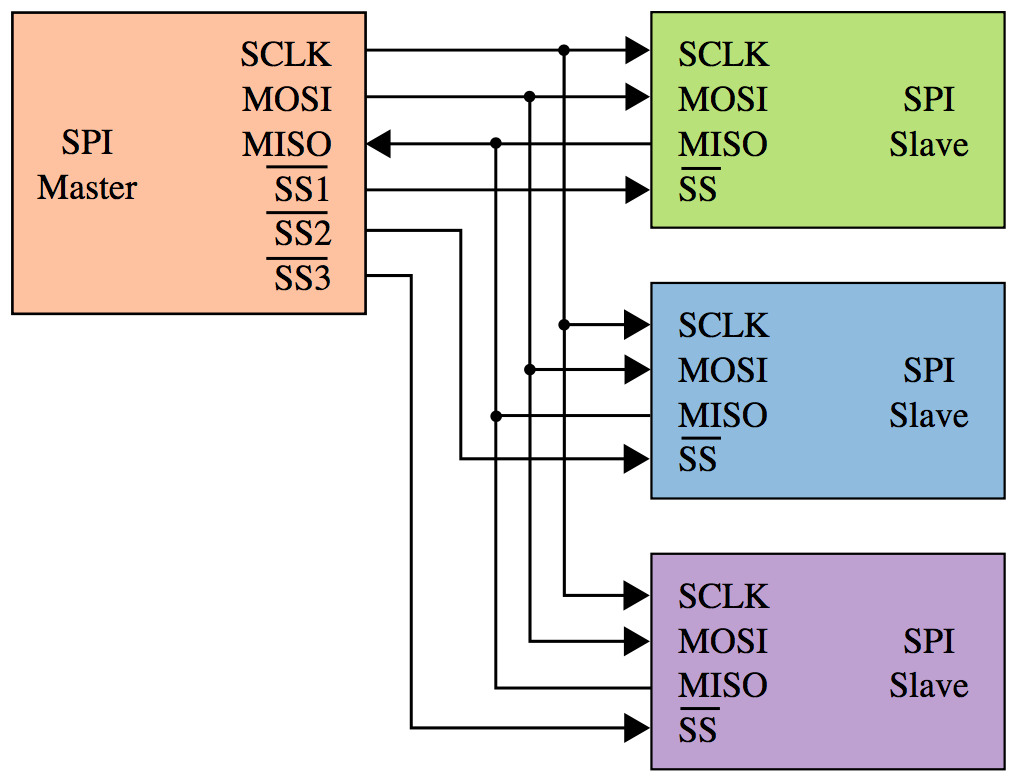
\includegraphics[max size={\textwidth}{\textheight}, scale=0.5]{Images/SPIdiagram.png}}
	\caption{Simple overview of SPI communication \cite{SPI}}
	\label{fig:SPIdiagram}
\end{figure}

\setlength{\parindent}{2.5ex} 
For the Smart Eraser system, the PSoC 6 is the master and the Arducam module is the slave. According to Arducam's data sheet, the Arducam SPI interface operates in SPI mode 0, meaning CPHA = 0 and CPOL = 0. Therefore the PSoC 6 is configured to operate in that mode as well. Also according the Arducam's data sheet the max frequency of its SPI interface is 8 MHz and therefore the PSoC 6 was configured to send a 7.142857 MHz signal to meet the requirement. Both the RX and TX of the PSoC 6 was set to be 16 bits wide in order to properly communicate with the Arducam SPI interface. An example of what the Arducam needs in order for proper communication can be found in Figure~\ref{fig:spiread} and Figure~\ref{fig:spiwrite}. The command byte, sent first, is structured so that the MSB is designated as the read/write byte, leaving the other 6 bits to represent an address in the Arducam SPI interface. The following byte is the data byte which contains specific data if the action is a write. If it is a read SPI transaction then this byte is known as a dummy byte because its just sent to push what needs to be read to master. The reason the TX and RX were set to 16 bits instead of 8 is because when this command and data byte is sent to the Arducam, the CS line needs to be asserted while both bytes are sent. When the PSoC 6 was configured with an 8-bit TX and RX, it would de-assert the CS line between each byte. This caused improper communication between the devices because from the point of view of the Arducam, it was only receiving command bytes.\par
\setlength{\parindent}{2.5ex}
This can be observed in the Arducam.C file, in any of the functions that use the Write\_SPI() function. A packet of 2 bytes is built and then placed into the TX of the PSoC 6 for transfer, which is handled by Write\_SPI(). These functions are: \\

\begin{itemize}
	\item MyCam\_Test(): Tests whether or not the SPI is working correctly 
	\item MyCam\_Trigger(): Function that initiates a capture 
	\item MyCam\_Check\_Capture\_Status(): Function that polls the capture ready flag in register 0x41 of the Arducam module. \\
\end{itemize}

\noindent \textbf{Code Implementation (Packet assembling):}\\ 
txBuffer = (((uint16\_t)WRITE + (uint16\_t)TEST\_SPI) << 8) + (uint16\_t)TEST\_VALUE;\\
\\\\
\textit{Code is from MyCam\_Test() in Arducam.C located in section ~\ref{A8}}\\\\

The Write\_SPI() function uses a combination of the APIs provided by Cypress in order to interact with the Serial Control Block 1(SCB1) that has been configured as aa SPI master. It is located in the I2Cmaster.C file found in ~\ref{A4}.

 \begin{figure}[H]
	\centering
	{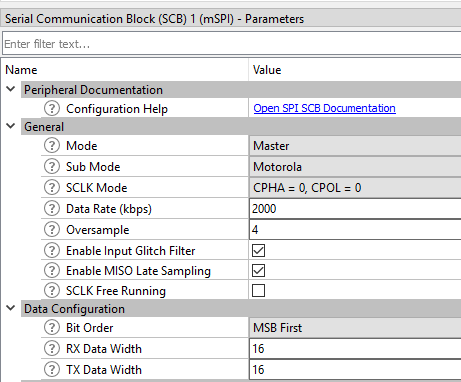
\includegraphics[max size={\textwidth}{\textheight}, scale=.9]{Images/SPIconfig1.png}}
	\caption{Hardware configuration of SPI (1)}
	\label{fig:SPIconfig1}
\end{figure}

\begin{figure}[H]
	\centering
	{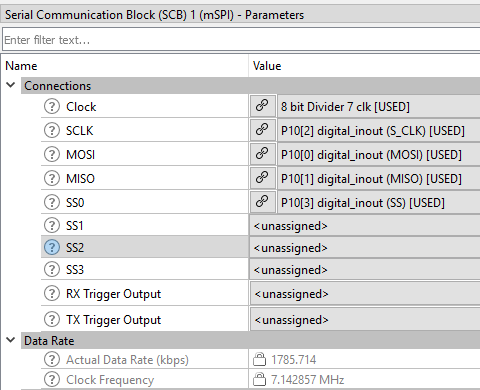
\includegraphics[max size={\textwidth}{\textheight}, scale=.9]{Images/SPIconfig2.png}}
	\caption{Hardware configuration of SPI (2)}
	\label{fig:SPIconfig2}
\end{figure}

\subsection{Image Processing}
\subsubsection{Resolution}
The original idea was to use a high-definition image to process because it would be able to capture more information, and therefore more accurately detect objects in a picture. This was assumed without taking into account the capabilities of the microcontroller. As it has been stated, attempts to add more physical memory to the system proved to more difficult than expected, leaving the program to only operate with a limited amount of memory. Due to this limitation, as well as matching the resolution of the TFT screen, a resolution of 320x240 was chosen to implement the image processing aspects of the system. It should be stated that the program was structured in a way that allows for easy changing of resolutions. Another impact of memory limitation is that only 80 rows of the image can be evaluated at a time. The resolution parameters are set in ImProc.H which can be found in section ~\ref{A11}.\\

\subsubsection{Output Format}
 There are a multitude of image formats than can be used and each one has its own specific way to read pixel information. JPEG was immediately decided against due to its lossy nature and high level of complexity to read pixel data. That left RGB, raw RGB, and YUV formats. Going a level down, each of the three formats have different arrangements and sizes in which they can be formed. For example, RGB can be either 888, 565, 555, 444, and even still further the ordering of the R,G, and B can vary.\par
\setlength{\parindent}{2.5ex} 
Cypress provides an example project that interacts with the TFT display and uses an example image with a format of RGB565 and resolution of 320x240. Since the Arducam can, if configured correctly (a whole project in itself), output this format with that resolution, pre loaded images with this formatting were used to test and develop the image processing aspects of the system. Without being able to see the results on the TFT display of what was being applied to the pixel data, the image processing program would have never worked correctly.\par
\setlength{\parindent}{2.5ex}
For the Smart Eraser system, as mentioned above, a format of RGB565 was chosen. Not only would images captured be able to be displayed on the TFT display, but the way in which the image data would be received from SPI communication would be relatively straightforward. Pixel information is broken up between 2 consecutive bytes, a high and low byte. Knowing how RGB565 is arranged, every two bytes of information received over SPI would be used to constructed one pixel of information and due to the nature of the SPI hardware configuration of the PSoC 6, each SPI transfer is 2 bytes. Therefore each SPI transfer consists of one complete pixel.

 \begin{figure}[H]
	\centering
	{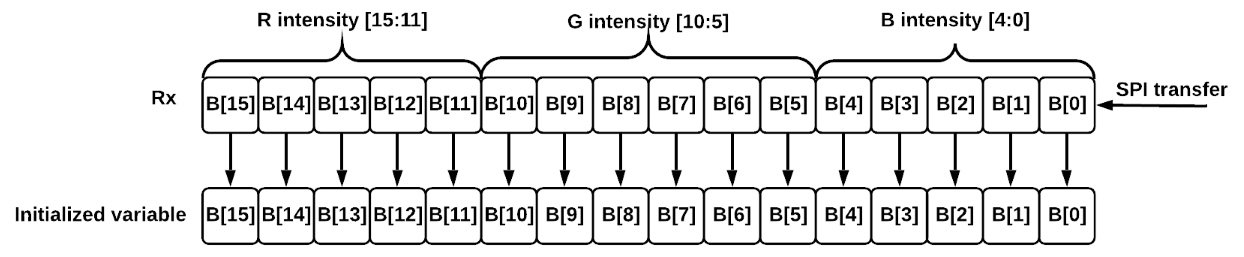
\includegraphics[max size={\textwidth}{\textheight}, scale=1]{Images/outputFormat.png}}
	\caption{Pixel Information being received through SPI from Arducam}
	\label{fig:outputFormat}
\end{figure}

\subsubsection{Resolution}
There are many different ways to do grayscale conversion from RGB. All are capable of achieving what was needed for Smart Eraser System, and the only difference between the methods are how true to gray the image looks and whether it has a darker or lighter tone to it. Because it is more accurate to the human eye, the Luminance method was chosen for the Smart Eraser system to convert to grayscale, mainly for the fact that the images would be viewed and not just processed behind the scenes.\par
Here is quick description of some different methods, including Luminance:\\

\begin{itemize}
\item Averaging Method
	\begin{itemize}
		\item  $ Gray = (Red + Green + Blue) $ 	\cite{Helland}
	\end{itemize}
\item Luminance Method
	\begin{itemize}
		\item $ Gray = (Red \times 0.2126 + Green \times 0.7152 + Blue \times 0.0722) $ \cite{Helland}
	\end{itemize}
\item Desaturation
	\begin{itemize}
		\item $ Gray = (Max(Red, Green, Blue) + Min(Red, Green, Blue)) / 2 $ \cite{Helland}
	\end{itemize}
\item Decomposition (Max or Min)
	\begin{itemize}
		\item $ Gray = Max(Red, Green, Blue) $ \cite{Helland}
		\item $ Gray = Max(Red, Green, Blue) $ \cite{Helland}
	\end{itemize}
\item Single Color Channel
	\begin{itemize}
		\item $ Gray = Red $ \cite{Helland}
		\item $ Gray = Green $ \cite{Helland}
		\item $ Gray = Blue $ \cite{Helland}\\
	\end{itemize}	
\end{itemize}

Once again, which method that is used is not important, it is separating the intensities from each other and then comparing them on an equivalent scale. An output format of RGB565 uses 16 bits to represent a single pixel, as shown in (figure with rgb565 output in previous section). In order to separate these intensities, the variable that contains the pixel information (type uint16\_t) is masked accordingly to pull out the R,G, and B intensities, storing them into new variables (type uint8). Masking is the process of performing a logical AND operation on a variable to isolate bit values contained in that variable. As demonstrated in Figure~\ref{fig:Seperate_Intensities} if the pixel data variable is ANDed with the Red Mask variable, only bits[15:11] will be retained.

\begin{figure}[H]
	\centering
	{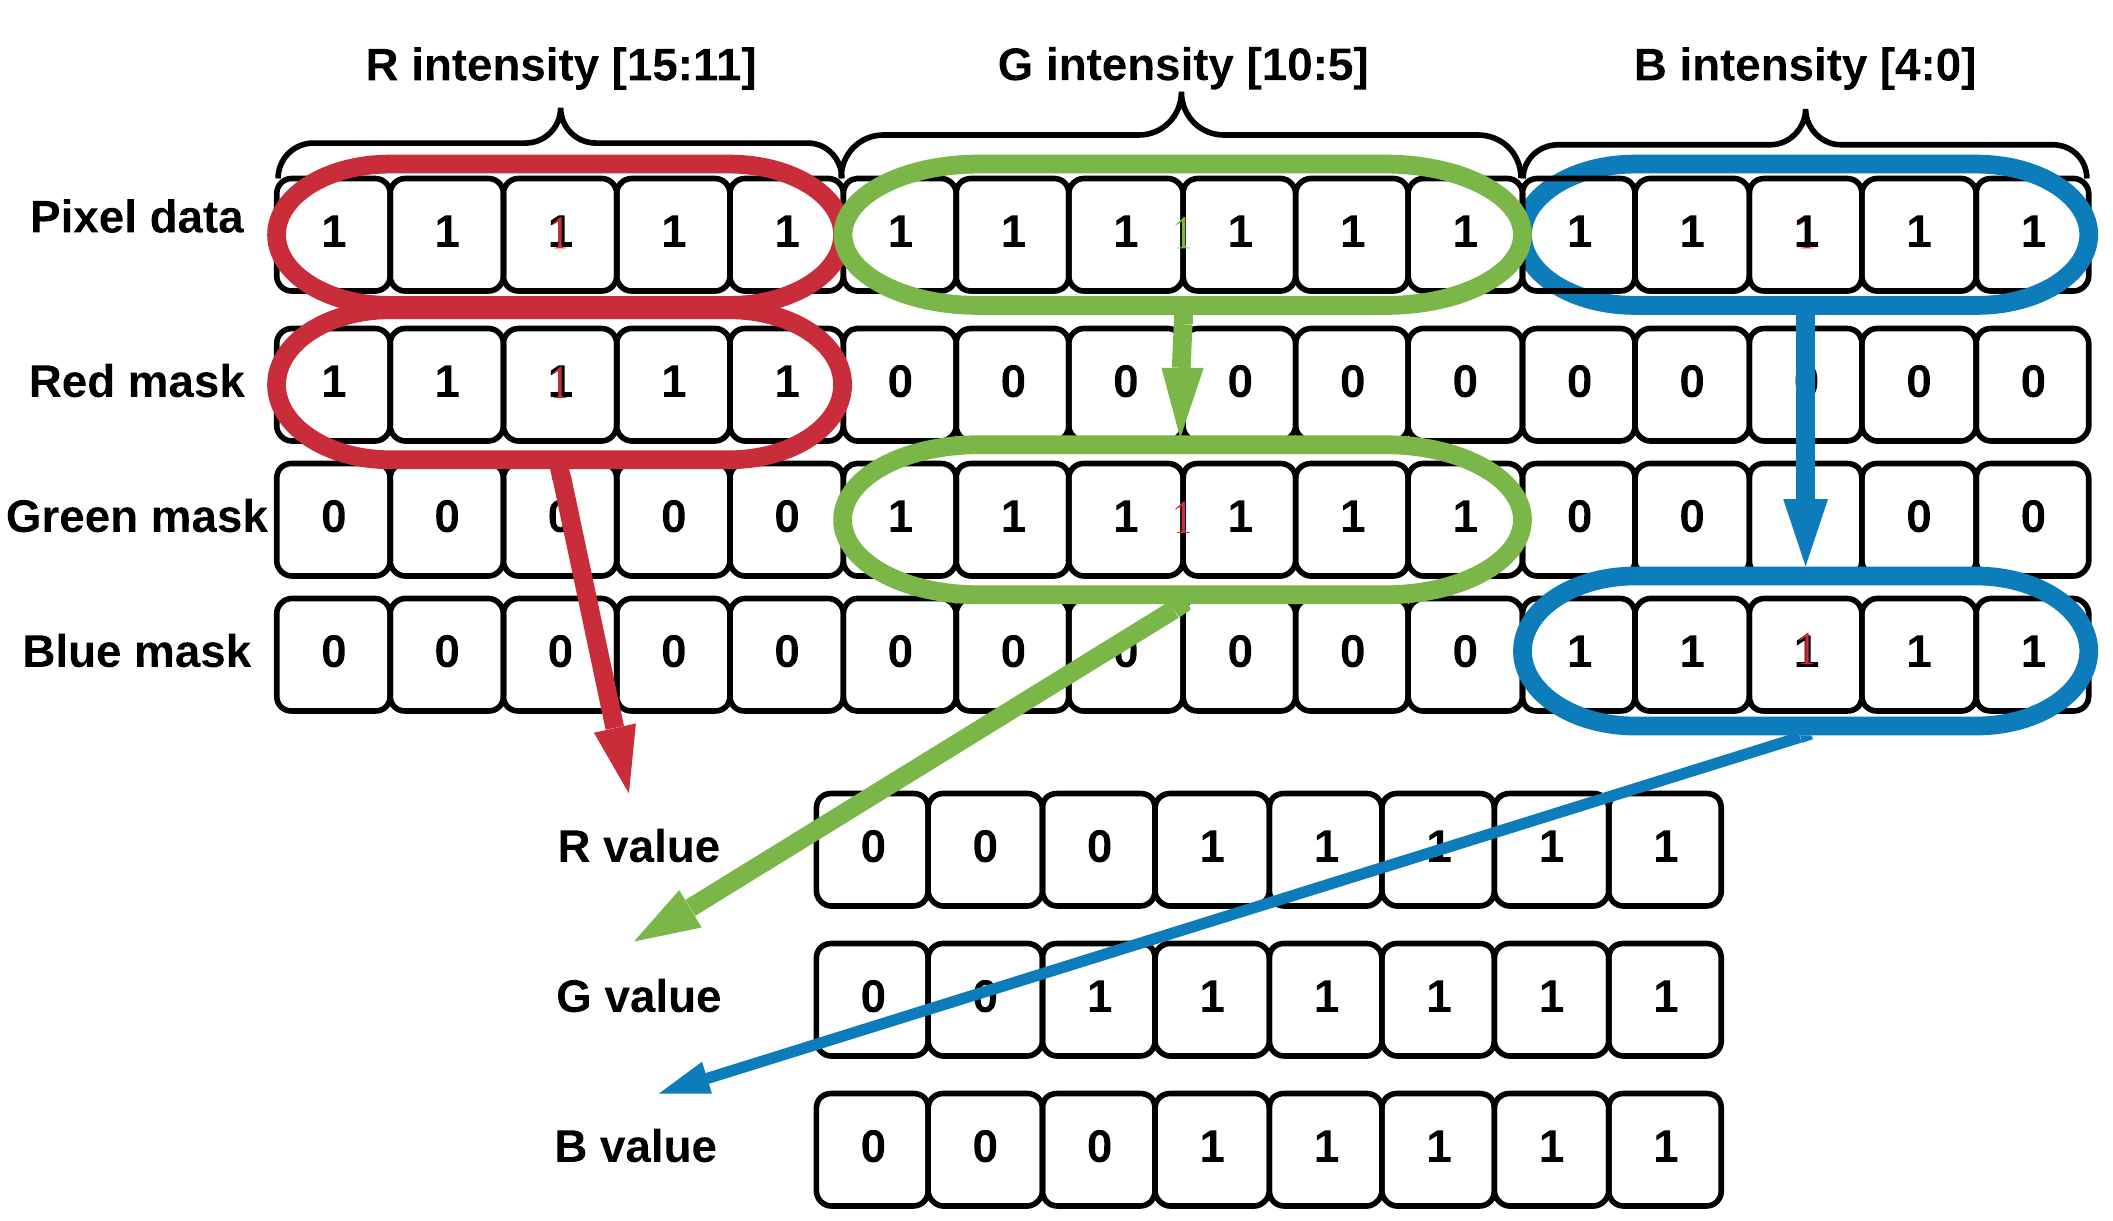
\includegraphics[max size={\textwidth}{\textheight}, scale=1]{Images/Seperate_Intensities.png}}
	\caption{How red, green, and blue intensities are seperated from one another}
	\label{fig:Seperate_Intensities}
\end{figure}

With the newly separated values as is, R and B represent shades of gray on a scale of 0 to 32 whereas G represents shades of gray on a scale of 0 to 64. If these values were to be used in one of the grayscale conversion algorithms, an image in shades of purple would be generated. This is known because it isn’t clearly stated anywhere that when using these conversion formulas, the intensities have to be represented by the same number of bits and therefore initial trials did not take this into account. Therefore some simple shifting is required before the formulas can be used. All intensities were upscaled to 8 bits so that values are compared on the complete range of grays (0 - 255) rather than descaling the green intensity down to 5 bits so that values are compared on a smaller, incomplete range of grays (0 - 32). 

\begin{figure}[H]
	\centering
	{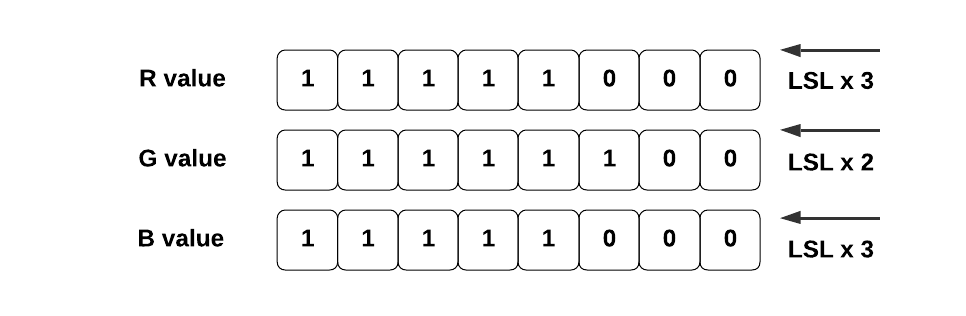
\includegraphics[max size={\textwidth}{\textheight}, scale=0.9]{Images/scaling.png}}
	\caption{Scaling seperated red green and blue intensities up to 8 bit numbers}
	\label{fig:scaling}
\end{figure}

\noindent \textbf{Code Implementation (Separation and scaling):}
\begin{lstlisting}
R 	= ((pixel \& 0b1111100000000000) >> 11 << 3);		 
G	= ((pixel \& 0b0000011111100000) >> 5 << 2);			
B	= (pixel \& 0b0000000000011111) << 3;
\end{lstlisting}
\textit{Code is from conv2gray() in ImProc.C located in section ~\ref{A10}}\\

At this point the RGB values are ready to be run through the conversion formula to generate a gray pixel value, in 8 bits. This gray value will then be used as the new R, G and B intensities of the original pixel, creating a shade of gray in the RGB565 format.  To build this new RGB565 pixel, the process up until now is done in reverse. New variables are created to hold “processed” values of RGB that are of type uint16\_t, to match the original pixel data length. 

\begin{figure}[H]
	\centering
	{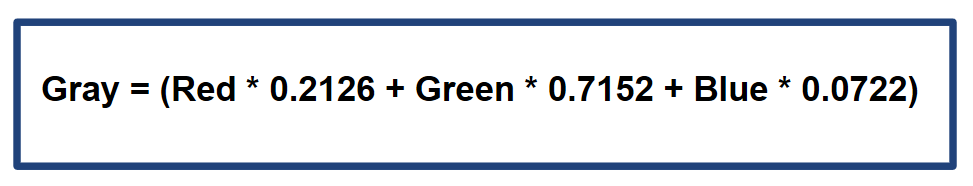
\includegraphics[max size={\textwidth}{\textheight}, scale=0.6]{Images/gray_equation.png}}
	\caption{Luminance method for converting RGB to grayscale}
	\label{fig:gray_equation}
\end{figure}

\begin{figure}[H]
	\centering
	{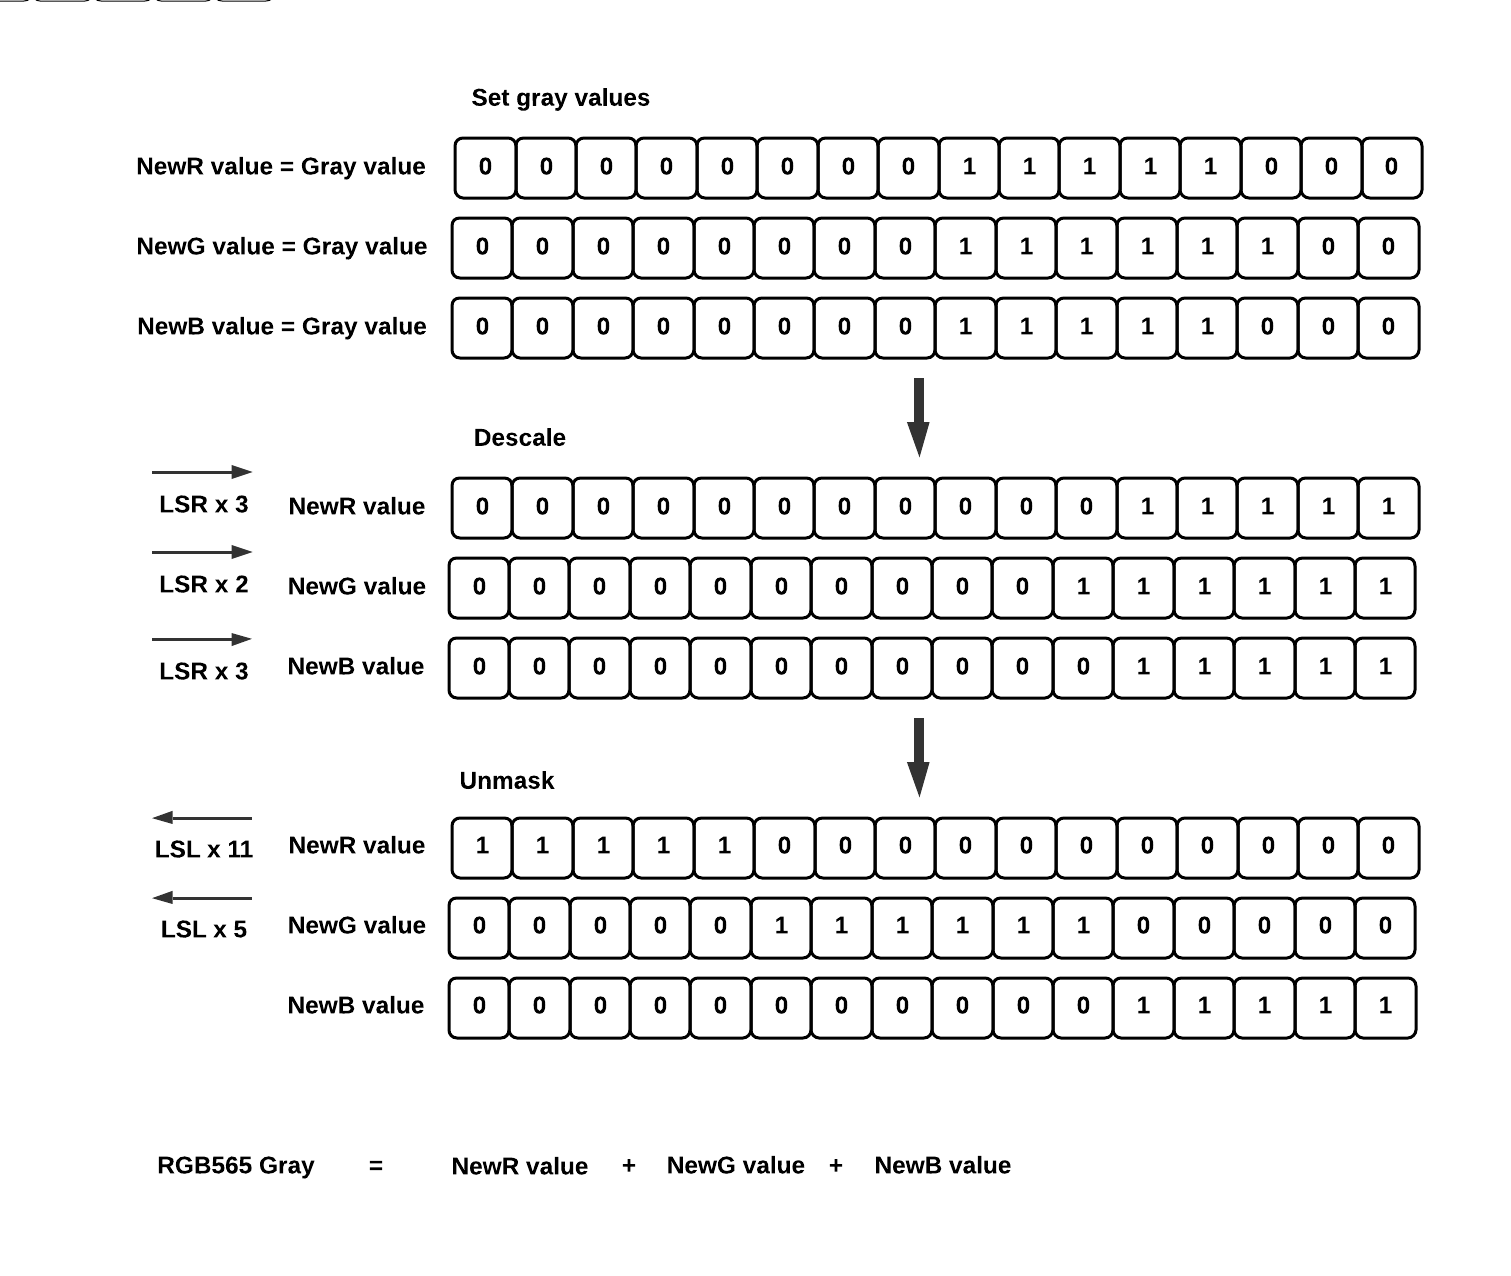
\includegraphics[max size={\textwidth}{\textheight}, scale=1]{Images/reverse.png}}
	\caption{Process in reverse: In order to create gray RGB pixel}
	\label{fig:reverse}
\end{figure}

\noindent \textbf{Code Implementation (conversion, descaling, reassigning):}
\begin{lstlisting}
Gray\_pixel = (R * 0.2126) + (G * 0.7152) + (B * 0.0722);		
R\_processed = ((uint16\_t)Gray\_pixel)>> 3 << 11;							
G\_processed = ((uint16\_t)Gray\_pixel)>> 2 << 5;							
B\_processed = (uint16\_t)Gray\_pixel >> 3;								
pixel = (uint16\_t)(R\_processed + G\_processed + B\_processed);
\end{lstlisting}

\textit{Code is from conv2gray() in ImProc.C located in section ~\ref{A10}}\\

\subsubsection{Grayscale Results}
\FloatBarrier
\begin{figure}[!htb]
	\centering
	{\includegraphics[max size={\textwidth}{\textheight}, scale=0.65]{Images/gray1.png}}
	\caption{Reuslts of grayscale algorithm from PSoC 6 (1)}
	\label{fig:results1}
\end{figure}
\FloatBarrier
\FloatBarrier
\begin{figure}[!htb]
	\centering
	{\includegraphics[max size={\textwidth}{\textheight}, scale=0.65]{Images/gray2.png}}
	\caption{Reuslts of grayscale algorithm from PSoC 6 (2)}
	\label{fig:results2}
\end{figure}
\FloatBarrier

\subsubsection{Sobel Edge Detection}
Sobel edge detection is an edge detection algorithm that uses a sobel kernel to detect differences in intensities at each pixel location. This is done by convolving a sobel kernel through each pixel in an image array. The pixel information must be grayscale in order for changes in intensity to be seen. A sobel kernel is a 3x3 array containing specific values to determine changes in values (gradients) from one edge to another. This has to be done for both vertical and horizontal edges, so there will be a kernel for each. The values inside the kernel are what make it a Sobel kernel. Using different values would classify it as a different type such as, Sobel–Feldman or Scharr. 

\begin{figure}[H]
	\centering
	{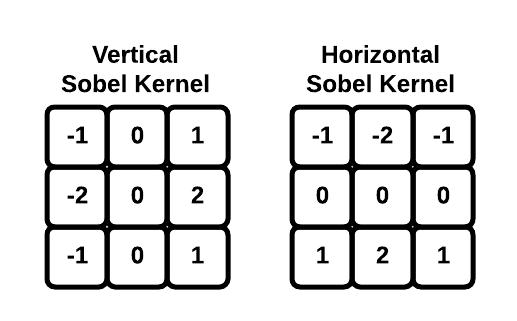
\includegraphics[max size={\textwidth}{\textheight}, scale=1]{Images/sobelKernel.png}}
	\caption{Sobel Kernels}
	\label{fig:sobelKernel}
\end{figure}

When moving through the image array, the center of the 3x3 kernel must never reach a border pixel otherwise a segmentation fault will prompt. This is because the pixel being evaluated (at the center of the kernel) relies on information from the surrounding pixels. If you were to attempt to pass the kernel through any part of the border, there will be some portion of the kernel that is out of bounds of the defined memory region. This is shown in Figure~\ref{fig:outofBounds}.

\begin{figure}[H]
	\centering
	{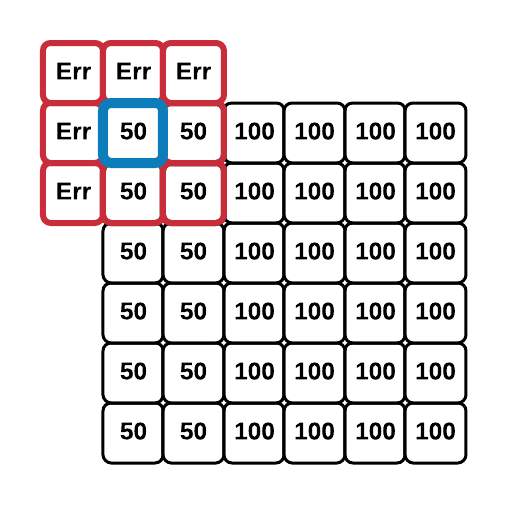
\includegraphics[max size={\textwidth}{\textheight}, scale=1]{Images/outofBounds.png}}
	\caption{Visual of what happens if the the sobel kernel is convolved along a boundary}
	\label{fig:outofBounds}
\end{figure}

\noindent \textbf{Code Implementation (boundary detection):} 
\begin{lstlisting}
for (k = Length + 1; k < bound - Length; k++){
		if ((k + 1) \% Length == 0) {
		ptr\_GD = ptr\_GD + 2;
		ptr\_PD = ptr\_PD + 2;
		k = k + 2;
}
\end{lstlisting}
\textit{Code is from sobel() in ImProc.C located in section ~\ref{A10}}\\\\
Once boundaries are accounted for in the program, the kernel can be convolved through the image array. At each pixel location (inside of boundary pixels) the operation shown in figure (right below) is carried out, both for the X and Y gradient.  

\begin{figure}[H]
	\centering
	{\includegraphics[max size={\textwidth}{\textheight}, scale=.75]{Images/sobelConV.png}}
	\caption{Operation of the vertical kernel}
	\label{fig:sobelConV}
\end{figure}

\begin{figure}[H]
	\centering
	{\includegraphics[max size={\textwidth}{\textheight}, scale=.75]{Images/sobelConH.png}}
	\caption{Operation of the Horizontal kernel}
	\label{fig:sobelConH}
\end{figure}

Finding the gradient in both the X and Y direction at any given pixel location (aside from boundary pixels) allows the total magnitude to be found at that location. This is done by taking the Gx and Gy values and using the Pythagorean Theorem. 

\begin{figure}[H]
	\centering
	{\includegraphics[max size={\textwidth}{\textheight}, scale=.55]{Images/Pythag.png}}
	\caption{Using Pythagorean theorem to determine the magnitude of the gradient}
	\label{fig:Pythag}
\end{figure}

\noindent \textbf{Code Implementation (kernel convolution):} 
\begin{lstlisting}
Gx =(sobel_kernel[0])*(*(ptr_GD  - Length + 1)) + (sobel_kernel[1])*(*(ptr_GD + 1)) 			+
	(sobel_kernel[2])*(*(ptr_GD  + Length + 1)) - (sobel_kernel[0])*(*(ptr_GD - Length - 1))    -
	(sobel_kernel[1])*(*(ptr_GD  - 1))			- (sobel_kernel[2])*(*(ptr_GD + Length - 1));

Gy =(sobel_kernel[0])*(*(ptr_GD  - Length + 1)) + (sobel_kernel[1])*(*(ptr_GD - Length)) 		+
	(sobel_kernel[2])*(*(ptr_GD  - Length - 1)) - (sobel_kernel[0])*(*(ptr_GD + Length + 1))    -
	(sobel_kernel[1])*(*(ptr_GD  + Length))	    - (sobel_kernel[2])*(*(ptr_GD + Length - 1)); 

G = (sqrt(pow(Gx,2) + pow(Gy,2)));
\end{lstlisting}

\textit{Code is from sobel() in ImProc.C located in section ~\ref{A10}}

The total magnitude G is now compared against a threshold value, which can be manipulated to adjust the strength of edge detection. If only sharp changes in intensity are desired, to be recognized as an edge then you would set the threshold value very high and if any change of intensity is desired then the threshold will be set very low. It is a trial and error to see if the image turns out correctly or not and is easily adjustable. Conditional statements are used to then compare against this threshold to set a pixel value to either white (detected edge, G is above threshold) or black (nothing detected, G is below threshold).

\subsubsection{Results of Sobel Edge Detection}
\textcolor{white}{This text is so the following figure will be below this heading!}

\begin{figure}[H]
	\centering
	{\includegraphics[max size={\textwidth}{\textheight}, scale=0.6]{Images/sobelResult.png}}
	\caption{Results of Sobel edge detection}
	\label{fig:sobelResults}
\end{figure}

\subsection{\textit{Square\_detection.c} Algorithm}
In order to begin the process of the eraser moving to the correct locations on the whiteboard, a rough detection of where the markings are located on the board needs to be found first. Using the array that the sobel edge detection algorithm produced, an algorithm was created to detect essentially the ``square'' in which the data was located. That is, it detects the top-most, left-most, bottom-most, and right-most locations of the white pixels in the finished array in order to create a virtual ``square'' around the data. The flowchart for the logic of the algorithm is shown in \ref{fig:squaredetect} in the \textit{Project Description and Boundaries} section of this report. See Figure~\ref{fig:serpentine} for a visual representation, with an example of the board being divided into an 8x8 grid. In this example, the ``square'' coordinates for the top, left, bottom, and right-most markings is 2, 3, 6, 7 respectively, with the origin of the x and y axis being at the top-left corner of the board. This is how the system will know where to erase the data. The blue-arrowed path in the next figure represents the serpentine.c program, which is explained in the \textit{Serpentine.c} Algorithm section of this report.

\begin{figure}[H]
	\centering
	{\includegraphics[max size={\textwidth}{\textheight}, scale=0.6]{Images/coordinate_algorithm_concept.png}}
	\caption{Visualization of \textit{square\_detection.c} and \textit{serpentine.c} working together to eraser markings on the whiteboard}
	\label{fig:serpentine}
\end{figure}

The actual code for this algorithm has been completed using a ``dummy'' matrix with random values of 0s and 1s representing blank space and markings. The code for this is in \textit{Appendix 3} of this report. The result with this dummy matrix is shown in Figure~\ref{fig:square_result}. This program is then combined with the \textit{serpentine.c} algorithm explained in the \textit{Serpentine.c Algorithm} section of this report.

\begin{figure}[H]
	\centering
	{\includegraphics[max size={\textwidth}{\textheight}, scale=0.8]{Images/square_dummy_result.png}}
	\caption{Result of \textit{square\_detection.c} program with the dummy matrix introduced within it for testing}
	\label{fig:square_result}
\end{figure}

\subsection{UART Communication - PSoC 6 to HUZZAH32 (server)}
Universal Asynchronous Receiver/Transmitter (UART) was chosen as the communication protocol between the main microcontroller (PSoC 6) and server microcontroller (HUZZAH32). This is the simplest of the three communication protocols used in the Smart Eraser. As the name suggests, communication is asynchronous, meaning there is no clock regulating the transfer of data between devices. Instead a baud rate is used, which is defined as the rate information can be transferred along a communication channel. Unlike SPI and I\textsuperscript{2}C, there is no master/slave relationship and thus communication relies on a few, simple parameters. Each device must be set to the same parameters in order to properly communicate. These parameters include; baud rate, parity, stop bit(s). The Smart Eraser system operates with a 115200 baud rate, parity enabled and set to even, with 1 stop bit and aheres to the RS232 standard of serial communication \cite{UARTstandard}.  

\begin{figure}[H]
	\centering
	{\includegraphics[max size={\textwidth}{\textheight}, scale=.95]{Images/UARTpacket.png}}
	\caption{UART packet contents \cite{UARTmessage}}
	\label{fig:UARTpacket}
\end{figure}

\noindent The original plan was to communicate with I\textsuperscript{2}C because the PSoC 6 already had a configured SCB for master I\textsuperscript{2}C transferring capabilities. However, due to limitations with the HUZZAH32 (currently only configurable as master (both SPI and I\textsuperscript{2}C)) UART was chosen instead. While researching UART it was found that this is often the chosen method of communication between MCUs so it worked out being the best option anyways. The code implementation of sending packets to the server (written in C) and how the server receives the packets (written in Python) is shown below:\\

\noindent \textbf{Code Implementation (UART TX):}
\begin{lstlisting} 
Cy_SCB_UART_PutArray(KIT_UART_HW, ptr_PD, 25);
Cy_SysLib_Delay(1);
Cy_SCB_UART_ClearTxFifoStatus(KIT_UART_HW, CY_SCB_UART_TX_DONE);
\end{lstlisting}
\textit{Code is from Process\_Image() in main.C located in section ~\ref{A3}}\\

\noindent \textbf{Code Implementation (UART RX):}
\begin{lstlisting} 
def UARTread():
  uart.init(9600, bits = 8, parity = 0, stop = 1, rx = 16, tx = 17)
  buff = bytearray(8)
  while not uart.any():
    pass
  uart.readinto(buff)
  uart.init(baudrate = 9600)
  return buff
\end{lstlisting}
\textit{Code is from UARTread() in UART.py located in section  ~\ref{A3}}

\subsection{The Original Plan for Wireless Communication}

When this project was originally started, the idea was to use wires to connect all of the components. This meant that a long wire would need to be used to connect the components on the Y-axis of the whiteboard in order to allow it to move. This idea was abandoned when everyone involved realized that not only would wireless communication allow for a more “pleasing to the eye” design, but would also add a layer of complexity to the project’s difficulty. \par
\setlength{\parindent}{2.5ex}
The original plan for the wireless communication was to use Raspberry Pi boards that would connect to the DE1\_SoC wirelessly via a wireless dongle that would plug into the DE1\_SoC. However, the transceivers that were found that would allow the Raspberry Pi boards to be wireless were only compatible with Arduino boards, so the Raspberry Pi was changed to Arduino. Soon after, problems arose from using the DE1\_SoC, so the microcontroller changed to the PSoC 6, and the new plan became to hardwire the transmitter Arduino to the PSoC 6. \\

\subsubsection{Arduino Wireless Communication}

Arduino microcontrollers are notoriously straightforward to use because of their open-sourced nature, meaning that there are already many libraries that are made for the board for various other external devices they can be used with, as well as applications that they can be used for. Therefore, the wireless communication between the transmitter and receiver Arduinos was straightforward, as well as the connections between the board and the transceiver. \par
\setlength{\parindent}{2.5ex}
The transmitter Arduino that would send instructions to the stepper motors was the model MKR1000, and the transceiver that could process the wireless communication and send the information needed was a Kuman nRF24L01 with an attachable antenna to extend the range that the wireless radio signal could reach. The pin layouts for the MKR1000 and the transceiver are shown in Figure~\ref{fig:mkr} and Figure~\ref{fig:trans1}.

\begin{figure}[H]
	\centering
	{\includegraphics[max size={\textwidth}{\textheight}, scale=0.8]{Images/arduino_mkr_back.jpg}}
	\caption{Image and pin layout of the MKR1000 WiFi module by Arduino \cite{mkr}}
	\label{fig:mkr}
\end{figure}
\begin{figure}[H]
	\centering
	{\includegraphics[max size={\textwidth}{\textheight}, scale=0.5]{Images/transceiver_pins.jpg}}
	\caption{Image and pin layout of the Kuman nRF24L01 transceivers\cite{trans1}}
	\label{fig:trans1}
\end{figure}

A diagram showing the connections between these two chips is in Figure~\ref{fig:conn1}.

\begin{figure}[H]
	\centering
	{\includegraphics[max size={\textwidth}{\textheight}, scale=0.7]{Images/Arduino_conn.png}}
	\caption{Pin connections between the MKR1000 microcontroller and the wireless transceiver to create the transmitter module}
	\label{fig:conn1}
\end{figure}

For the code of the transmitter, the template code was taken from the example shown by Dejan Nedelkovski, and is shown in Appendix 1 of this report. In order to use the wireless transceiver, the specific library made for it needed to be included. The RF24 radio was then configured to use pins 6 and 7 on the Arduino as the CE and CSN pins shown in Figure~\ref{fig:trans1}. In the setup of the program, the radio connection is initialized, the PA level is set to the minimum it can be, and the radio is set to be a transmitter with the stopListening() function. The addresses the transmitter will be sending data to are also outlined. The PA is the Power Amplifier factor, and the higher it is, the more unstable it can be, which would then require a bypass capacitor to be connected between the voltage power source and ground connected to the chip. Therefore, it was kept to a minimum, especially because the modules were so close together, so it was unnecessary to amplify it more.\par
\setlength{\parindent}{2.5ex}
Next, in the main loop of the program, in order to send a signal to a specific address, a writing pipe needs to be opened to that address. Only one writing pipe can be open at a time, so separate writing pipes to each receiver were opened and continuously alternated between in the loop. The number for the stepper motors to rotate a certain degree were then sent using the radio.write() function, whos parameters include a pointer to the name of the variable to send to the receiver, and the length of the data.\par
\setlength{\parindent}{2.5ex}
The receivers that were attached to each stepper motor were the Arduino UNO R3, and the transceivers were the same model used for the transmitter. The Arduino UNO R3 used is shown in Figure~\ref{fig:uno}.

\begin{figure}[H]
	\centering
	{\includegraphics[max size={\textwidth}{\textheight}, scale=1.2]{Images/uno_r3.png}}
	\caption{Pin layout on the Arduino UNO R3 \cite{uno}}
	\label{fig:uno}
\end{figure}

The pin connections between the UNO R3 and the wireless transceiver are shown in Figure~\ref{fig:conn2}.

\begin{figure}[H]
	\centering
	{\includegraphics[max size={\textwidth}{\textheight}, scale=0.8]{Images/Arduino_conn2.png}}
	\caption{Pin connections between the UNO R3 microcontroller and the wireless transceiver to create the receiver modules}
	\label{fig:conn2}
\end{figure}

For the code of the receiver, the template code was taken from the example shown by Dejan Nedelkovski, and is shown in Appendix 2 of this report. In order to use the wireless transceiver, the specific library made for it needed to be included. The RF24 radio was then configured to use pins 9 and 10 on the Arduino as the CE and CSN pins. In the setup of the program, the radio connection is initialized, the PA level is set to the minimum it can be, and the radio is set to be a receiver with the startListening() function. The address of the receiver is set, and the baud rate is also set for the Serial Monitor within the Arduino IDE so it will read in data at the specified rate. Next, in the main loop of the program, a loop is created to check if there is data available to receive. If there is, the data is read into a variable to be used for the stepper motor movement.\par
\setlength{\parindent}{2.5ex}
When both of these programs ran, they each received the instructions wirelessly and were able to move the stepper motors the right degree of rotation. However, unfortunately, due to an unknown reason the wireless communication stopped working with about 30 days left to complete the project. The most likely culprit for the malfunction may have been due to faulty transceivers; upon further inspection of the reviews left by those who have used these devices in the past, many did not work correctly upon arrival. Therefore, this method of wireless communication had to be replaced with three HUZZAH32 Feather boards by Adafruit, with one being used as a host server (a.k.a. the transmitter) and two being used as clients to the server (a.k.a. the receivers). This leads to the current wireless communication system, which is a connection between a `host' or `server' (which acts as the transmitter) and the `client' (which acts as the receievr).\\


\subsection{The Current Wireless Communication System}
The decided upon wireless communication system was to use a client/server implemented on HUZZAH32s. One would act as the server, directly interacting with the PSoC 6 and the other two would be clients, attached to the stepper motor systems. Using micropython, the server uses libraries and socket programming in order to achieve this. Both clients and server will be set up as stations and a router will be used in order for the server to talk to the clients. There are few things that are necessary in order for this to work. There needs to be two separate IP addresses for the network and server as well as defining a port on the server side so that the clients know what to look for. Lastly, as this is a TCP connection, there must be acknowledgment for every packet sent. These ACKs are handled behind the scenes through the Python socket library. 

\begin{figure}[H]
	\centering
	{\includegraphics[max size={\textwidth}{\textheight}, scale=0.55]{Images/socket.png}}
	\caption{Overview of client/server interaction \cite{socket}}
	\label{fig:socket}
\end{figure}

\subsubsection{Server}
The HUZZAH32 used for the server is connected to the PSoC 6 through UART so that it can receive the results generated from \textit{Square\_Detection.c} that runs on the PSoC 6. After initialization is done and the socket is listening for connections, it will stay in an infinite \textit{while loop} to wait for both clients to connect. Each client that connects creates a new client thread on the server. Since there are a maximum of two clients, there will only ever be 2 threads running alongside the main. This worked out for the Smart Eraser system as the HUZZAH32 is much better at working as a client than a server handling multiple clients due to threading limitations in the current firmware. After exactly 2 client threads have been created, the main loop then waits for information to come in over UART. A \textit{UARTread()} function is called which waits in a passing loop until information is received. When data is detected through UART, the incoming data is stored into a byte array and returned to the main function. This process can be seen in Figure~\ref{fig:Server}.

\begin{figure}[H]
	\centering
	{\includegraphics[max size={\textwidth}{\textheight}, scale=0.8]{Images/Server.png}}
	\caption{Flowchart of how the Server code works}
	\label{fig:Server}
\end{figure}

The client threads wait on this information before they can move any further. Both threads have access to the global byte array that stores the information incoming from UART. As soon as this array is not empty, the threads attempt to acquire the lock. Whichever one doesn't will have to wait until the other one is done sending its information, at which point the lock will be released. This is so that the micro controller does not become overwhelmed with too many parallel processes happening at once. This process happens for each 1/3 of the image that is processed meaning there will be three blocking calls in each thread to received all the information from each section. After the third byte array is received and both threads send the necessary data, each thread will exit (terminate). The only process running at this point should be the main thread waiting for two more client connections, starting the process all over again.\\\\

\noindent \textbf{Code Implementation Server (main thread):}
\begin{lstlisting}
while 1:
 k = 0
 while (k < 2):
  conn, addr = s.accept()
  print('Connected with ' + str(addr[0]) + ' : ' + str(addr[1]))
  start\_new\_thread(clientthread ,(conn, addr))
  k = k + 1
 self.List1 = []
 self.List2 = []
 self.List3 = []
 self.List1 = UARTread()
 self.List2 = UARTread()
 self.List3 = UARTread()
 time.sleep(5)
 self.List1 = []
 self.List2 = []
 self.List3 = []
 k = 0
\end{lstlisting}
\textit{Code is from SMserver.py located in section ~\ref{A16}}\\

\noindent \textbf{Code Implementation Server (client threads waiting for UART):}
\begin{lstlisting}
while self.List1 == []:
 pass  
while not lock.acquire():
 pass
print(self.List1)  
#Send first set of instructions
conn.sendall(self.List1)
time.sleep(2)
lock.release()
\end{lstlisting}
\textit{Code is from SMserver.py located in section ~\ref{A16}}\\

\subsubsection{Clients}
The two other HUZZAH32's will be used to act as clients, receiving information from the server that will be used to set variables for stepper motor movement. The information being received is in the form of byte arrays, which need to be converted for mathematical operations. Although the solution is quite simple, it took some major digging to come across a solution that was straightforward and actually worked. Most solutions were not able to be implemented with micro python. Thanks to user JohanL on a stack overflow forum under the topic ``Convert python byte ``array'' to int ``array \cite{JohanL}, we were able to convert the byte array to useful data. It turns out that the list constructor in python can translate a bye array into data that can be used with math operations. Therefore, a list was created out of the byte array information received from the server. Once the client has 3 lists of information from the server, they run the \textit{serpentine()} function corresponding to the three different sections in the image.

\noindent \textbf{Code Implementation Server (client threads waiting for UART):}
\begin{lstlisting}
while self.List1 == []:
 pass  
while not lock.acquire():
 pass
print(self.List1)  
#Send first set of instructions
conn.sendall(self.List1)
time.sleep(2)
lock.release()
\end{lstlisting}
\textit{Code is from SMclientX.py located in section ~\ref{A17}}\\

\subsubsection{\textit{Serpentine.c} Algorithm}

After finding the square in which all the data is contained on the whiteboard, another algorithm takes the edges of the square detected and creates a series of instructions for the stepper motors. The logic flowchart of this algorithm is shown in Figure~\ref{fig:serp} These instructions are the number of rotations needed to move the stepper motors in a certain direct, and are given to each motor serially to take a similar path to the one shown in Figure~\ref{fig:serpentine}. First, the motors are given the instructions to move to the top-left space of the data square. Then, the X-axis motor is continually given instructions to move from the far left side of the square to the far right of it, and the Y-axis motor is continually given instructions to move down one rotation in order to traverse down the square until all the material is erased. The algorithm then checks to see if the eraser stopped on the right side or the left side of the square based on how many rotations it needed to take to erase the markings. Based on this position, it gives the final instructions to the stepper motors to move the eraser back to its stand-by position at the top left of the entire whiteboard to await the next instructions sent to it.
When this program is ran with dummy values, it sends the correct sequence of instructions to the x and y stepper motors in the format of the number of rotations it needs to take if it were traversing the same dummy matrix from the \textit{square\_detection.c} algorithm.

\begin{figure}[H]
	\centering
	{\includegraphics[max size={\textwidth}{\textheight}, scale=0.8]{Images/serpentine_dummy_result.png}}
	\caption{Result of \textit{serpentine.c} program with the dummy values introduced within it for testing}
	\label{fig:serp_result_dummy}
\end{figure}


\subsubsection{Stepper Motor Movement}
The stepper motors that were chosen for this project are the NEMA 23 CNC stepper motors. Stepper motors contain magnetic coils surrounding a magnetic rotor that need to be powered in a certain sequence in order for the rotor to turn in either a clockwise (CW) or counter-clockwise (CCW) rotation. This particular stepper motor is a 2-phase bipolar motor, meaning it contains 2 groups of coils, and it uses all coils within the motor to work to turn the motor the direction needed. A layout of the inside of this motor is shown in Figure~\ref{fig:rotor}, which shows how the coil windings are oriented in comparison with the rotor. The different color names represent the colors of the wires that need to be connected to the stepper motor driver.

\begin{figure}[H]
	\centering
	{\includegraphics[max size={\textwidth}{\textheight}, scale=0.6]{Images/rotor.png}}
	\caption{Rotor and coil layout in the bipolar 2-phase NEMA 23 stepper motor}
	\label{fig:rotor}
\end{figure}

The specific combination of pulses in the order they need to be for CW and CCW motion are shown in Figure~\ref{fig:smdata} in this report. The pulse configurations shown in this figure allow the code to begin to be formed in order to rotate the stepper motors in the directions needed. The colors that correspond to the A, B, A\, B\ input leads are shown in the next figure.

\begin{figure}[H]
	\centering
	{\includegraphics[max size={\textwidth}{\textheight}, scale=0.6]{Images/bipolar_table.png}}
	\caption{Labeling of lead colors corresponding to winding inputs}
	\label{fig:bipolar}
\end{figure}

Because of the libraries included in the Arduino library, the code for the stepper motors was as simple as initializing the stepper motor pins being used as shown in Appendix 2, setting the speed in the initialization loop, then putting the number of rotations per minute into the function defined. However, because the wireless communication unfortunately stopped working, the code for the stepper motors to move needed to be redone in Micropython in order to allow the motors to move with the new HUZZAH32 boards being used for the wireless communications.\par
\setlength{\parindent}{2.5ex}
With the HUZZAH32 microcontrollers, the stepper motor code is also straight forward, as the coding language they use is Micropython. In this language, the code is as simple as putting the correct phases in 4 steps (as shown in Figure~\ref{fig:smdata}) by listing them as numbers in an array, then sending those steps to the stepper motor serially. If the motor needs to rotate in the counter clockwise direction, the array with the 4 steps can be reversed using the \textit{.reverse()}. A check condition checks for a negative number in order to perform this operation. The code for this part is in \textit{Appendix 15} of this report. The results of this code running are the stepper motors rotating depending on the number put into the variable `x'. \\

\subsubsection{HC-SR04 Ultrasonic Sensor}
The HC-SR04 is an ultrasonic sensor that can detect objects between the range of 2 cm to 4 m. To detect objects, a pulse is sent via the trigger pin (minimum of 10 µs), which triggers an 8 cycle 40 kHz burst of ultrasound. The time it takes to receive the echo of that burst can be used to calculate the distance of the object. Because the frequency is relatively high, the HC-SR04 Is a shorter-range sensor (4m is approximately 13 feet). This means that to increase the range of detection, the frequency would need to be lowered. The sensor needs to be connected to a microcontroller and be provided with 5V (not 3.3V), a ground, and 2 connections to GPIO pins (for the trigger and echo signals). 

\begin{figure}[H]
	\centering
	{\includegraphics[max size={\textwidth}{\textheight}, scale=0.6]{Images/Ultra.jpg}}
	\caption{How the ultra sonic sensor works \cite{Ultra1}}
	\label{fig:Ult1}
\end{figure}

\noindent \textbf{Code Implementation Ultra Sonic Sensor:}
\begin{lstlisting}
while self.List1 == []:
pass  
while not lock.acquire():
pass
print(self.List1)  
#Send first set of instructions
conn.sendall(self.List1)
time.sleep(2)
lock.release()
\end{lstlisting}
\textit{Code is from SMclientX.py located in section ~\ref{A17}}

\subsection{Hardware}
\subsubsection{Using the Logic Analyzer}
The logic analyzer is vital to figuring out how data is actually being transferred between interfaces. The I\textsuperscript{2}C, SPI and UART communications that were developed for the Smart Eraser system would not have been successfully implemented without using the logic analyzer. While creating the software to interact with these communications the need for APIs was needed in order to do so. Some of these APIs are not 100\% descriptive of what they actually do and was only discoverable through using the analyzer. Figure~\ref{fig:LA} shows results of a finally sending and receiving information over SPI successfully. 

\begin{figure}[H]
	\centering
	{\includegraphics[max size={\textwidth}{\textheight}, scale=1]{Images/LA.png}}
	\caption{SPI analysis using the logic analyzer}
	\label{fig:LA}
\end{figure}

\subsubsection{Stepper Motor and Driver Connections}
In order to drive a stepper motor, an H-Bridge needs to be used in order for current to flow to the correct coils, which supply the amperage needed to rotate the internal magnetic coil. In this project, the DM542T stepper drivers act as the H-bridge needed. The four different-colored leads (black, green, red, blue) are plugged into the A+, A-, B+, B- nodes, respectively. These nodes will send out the proper pulse signals to the stepper motor, as well as the voltage and current needed to drive them, depending on the inputs given to the PUL and DIR nodes. The PUL+, PUL-, DIR+, and DIR- nodes are connected to the HUZZAH32 Feather board in order to control the stepper motors. These signals are those that need to be coded into the microcontroller in order to be the control behind the motors. The PUL nodes control the pulse signals sent to the bipolar motor coils, and the DIR nodes control the direction of the flow of current into the coils, thus allowing the motors to run both CW and CCW. The driver used is shown in Figure~\ref{fig:smdataD}.

\begin{figure}[H]
	\centering
	{\includegraphics[max size={\textwidth}{\textheight}, scale=0.5]{Images/smD.png}}
	\caption{Stepper motor driver for the NEMA 23 \cite{smdataD}}
	\label{fig:smdataD}
\end{figure}

The stepper driver is able to be modified to alter the current flowing out to the stepper motors. The amperage supplied to the motors is directly proportional to the amount of torque the motors can provide. The Y-axis stepper motor driver's configuration allowed 1A to flow to the motor, and it was able to pull the weight attached to it. However, because there is a heavier load on the X-axis motor, the configuration had to be changed to allow more current to flow to get more torque to pull the extra weight without difficulty. That driver was set to the next setting up, which is 1.46A, and this allowed it to pull the extra weight fine. The max tolerance of current the motors can take is 2.8A, so if more weight was added as well, the motors would more than be able to handle it.

\subsubsection{Power Parameters}

The power rating for each component was important to take into account when thinking about the power supplies for the wireless components. The stepper motors are rated to have a driving voltage of anywhere from 24-48V, and the stepper drivers a driving voltage of 20-50V. Taking the mobility of the components into account, the final decision for the power sources for the different stepper motor components on the whiteboard wound up being three 9V batteries in series for one setup. Ideally, there would be 27V flowing to each stepper motor through the stepper drivers, but when measured in the lab, it wound up being about 24V flowing to each motor system. This is plenty to move the motors the way they need to, so this is the method that was chosen. For the other setup, a more stable power source will be used. This was decided for two reasons: the first being that the X motor system will not be moving, so it can have a dedicated power system that doesn't move, and can therefore be plugged into a power outlet if need be. The second reason for this decision was because the X motor needs a higher current due to the higher torque needed to move the heavier load of the Y-axis components. The following equation can be used to understand the power consumption parameters that were taken into account when making sure the batteries would provide enough current for the mobile part of the system. Figure~\ref{fig:power_supply} shows an image of the separate power supply.\\

\begin{center}
	$ Power Consumption = E_{kWh/day} = \frac{P_{(W)} \times t_{(h/day)}}{1000_{W/kW}} $
\end{center}

\begin{figure}[H]
	\centering
	{\includegraphics[max size={\textwidth}{\textheight}, scale=0.8]{Images/power_supply.png}}
	\caption{TDK Lambda power supply \cite{smdataD}}
	\label{fig:power_supply}
\end{figure}

\subsubsection{Printed Circuit Boards (PCBs)}

In order to connect everything in the original configuration of the wireless communication system, PCBs were made to ensure loose wires would not detract from the overall look of the final prototype. These PCBs were made for each stepper motor in order to connect the wireless transceivers, the Arduino UNO R3 microcontrollers, a 9V battery to the Arduino board for wireless power, and to connect the 3 9V batteries in series that would have powered the stepper motor drivers. Figure~\ref{fig:pcbs} shows the layout of the PCBs.

\begin{figure}[H]
	\centering
	{\includegraphics[max size={\textwidth}{\textheight}, scale=0.8]{Images/PCB_layout.png}}
	\caption{Layout of PCBs}
	\label{fig:pcbs}
\end{figure}

Figure~\ref{fig:pcb_b} and Figure~\ref{fig:pcb_a} show a before and after shot of what the components looked like connected before and after using the PCBs. They are much more organized and pleasing to the eye to look at.

\begin{figure}[H]
	\centering
	{\includegraphics[max size={\textwidth}{\textheight}, scale=0.6]{Images/pcb_before.jpg}}
	\caption{Connection of stepper motor system before PCBs}
	\label{fig:pcb_b}
\end{figure}
\begin{figure}[H]
	\centering
	{\includegraphics[max size={\textwidth}{\textheight}, scale=0.6]{Images/pcb_after.jpg}}
	\caption{Connection of stepper motor system after PCBs}
	\label{fig:pcb_a}
\end{figure}

Unfortunately, because the wireless transceivers stopped working three weeks before the project needed to be completed, the PCBs were not used in the final version of the product.

\subsection{Project Prototype - Planning}

This section contains all information about the conception, creation, and finalization of the prototype stand for the Smart Eraser to be mounted on.\\

\subsubsection{Initial Prototype Design}

Figure~\ref{fig:prtrough} and Figure~\ref{fig:prtsiderough} show the initial conception of the prototype stand, as well as some rough dimensions.

\begin{figure}[H]
	\centering
	{\includegraphics[max size={\textwidth}{\textheight}, scale=0.6]{Images/prototype_stand_rough.png}}
	\caption{A rough initial image of the prototype}
	\label{fig:prtrough}
\end{figure}
\begin{figure}[H]
	\centering
	{\includegraphics[max size={\textwidth}{\textheight}, scale=0.6]{Images/prototype_rough_side.png}}
	\caption{A rough side view with dimensions of the prototype}
	\label{fig:prtsiderough}
\end{figure}

These images helped to think of how large the stand should be.\\

\subsubsection{Final Prototype Design and Dimensions}

After the initial conception of the prototype stand, more definitive dimensions were found for the different components that would be connected to the board. Figure~\ref{fig:sideview} and Figure~\ref{fig:frontview} show the more detailed dimensions, as well as a more detailed figure that shows where everything would be placed relative to each other.

\begin{figure}[H]
	\centering
	{\includegraphics[max size={\textwidth}{\textheight}, scale=0.65]{Images/front_view.png}}
	\caption{The front view of the prototype stand schematic}
	\label{fig:sideview}
\end{figure}

\begin{figure}[H]
	\centering
	{\includegraphics[max size={\textwidth}{\textheight}, scale=0.5]{Images/side_view.png}}
	\caption{The side view of the prototype stand schematic}
	\label{fig:frontview}
\end{figure}
The prototype stand stands about 7 feet tall, but the whiteboard itself is lined up so the top is level with about 6 feet off the ground. This height was chosen in order to have the whiteboard at a position in front of the user so they wouldn't need to strain to write on it. Looking at the side view image of the dimensions of the whiteboard, there are two 2''x4'' posts on each side of the wooden backing to hold the board up: one attached to the front of the board, and one attached at the same place as the other, but on the back of the board. This design was chosen with the stress being placed on one post in mind; too much stress on one of the posts would result in a more unstable design, especially with the moving parts on the board. At the bottom of these posts are more 2''x4'' posts that are parallel with the ground that measure a little over half of the height of the entire prototype. This length was decided upon in order to ensure there was enough room to attach two more 2''x4'' posts at a 45 degree angle to the vertical 2''x4'' and the horizontal 2''x4'' to enable it to be more sturdy. The horizontal posts have wheels attached to the bottom of them so the prototype stand can be mobile, as it needs to be brought to the Satellite Student Union for Projects Day. Finally, the plywood that everything (the whiteboard, the tracks, the stepper motors and drivers, etc.) is attached to was limited one side only being 48'', so this was decided to be the height of the device. The original width of the board was 96'', but it was cut down to 66'' in order to allow room for the 2''x4''s to attach to the board, as well as the stepper motors, their drivers, and the PCBs. Three separate 2''x3'' pieces of wood were also cut and put on the back of the plywood to prevent the plywood, and subsequently the components being mounted to it, from warping due to instability or weather conditions when it is taken outside to go to the Satellite Student Union on Projects Day. \par
\setlength{\parindent}{2.5ex}
After finishing the conception of the prototype, building it and putting everything together came next.

\subsection{Project Prototype - Building}
Building the prototype took approximately 3 days; one day for connecting all of the wood pieces, and 2 for connecting all of the tracks, stepper motors, and making sure they would all be able to work together if motors rotated the pieces. An additional day was needed a couple weeks later to mount the smaller pieces, including the motor drivers and power systems. The following sections detail the steps that were took to put the system together, and they also contain images of the finished product.

\subsubsection{Component Mounting Steps}

The following list contains the steps that were followed when putting the stand together.

\begin{enumerate}
	\item Take measurements and sketch lines to cut the wood.
	\item Cut the plywood to be 48''x66'' at Home Depot.
	\item Cut the 2''x4'' posts at all necessary lengths, widths, and angles.
	\item Cut the 2''x3'' posts for the stability of the unit to their appropriate lengths.
	\item Drill and screw together the posts to the plywood.
	\item Drill and screw together the horizontal posts to the bottom of vertical posts so the stand can actually stand.
	\item Drill and screw together the 2''x3'' posts to the back of the board.
	\item Take measurements for the housing of the X-axis track (the board between the plywood and the track).
	\item Cut the leftover posts and drill and screw them onto the plywood.
	\item Drill the wheels to the bottom of the stand.
	\item Drill the holes into the X and Y-axis tracks to mount onto the board, and mount onto the carriages of the X-axis.
	\item Mount the stepper motors.
	\item Mount the flange on the opposite side of the tracks.
	\item Wrap the pulley belt around the stepper motors and the flanges.
	\item Attach belt to carriages with washers and nuts so the axes will actually move when the stepper motor rotates.
	\item Attach the braces to the Y-axis carriage to create a clamp to hold the eraser.
	\item Attach the smaller pieces (including the stepper motor drivers, power systems, etc.) to the board.
\end{enumerate}

\subsubsection{Final Product}

The final product in progress showing how the components were mounted to the front of the board, as well as the finished final product, are shown in Figure~\ref{fig:ipboard}, Figure~\ref{fig:actualfront}, and Figure~\ref{fig:actualside}.

\begin{figure}[H]
	\centering
	{\includegraphics[max size={\textwidth}{\textheight}, scale=0.65]{Images/in_progress_board.jpg}}
	\caption{The building of the prototype stand in progress}
	\label{fig:ipboard}
\end{figure}

\begin{figure}[H]
	\centering
	{\includegraphics[max size={\textwidth}{\textheight}, scale=0.65]{Images/actual_front.jpg}}
	\caption{The front view of the actual prototype stand}
	\label{fig:actualfront}
\end{figure}

\begin{sidewaysfigure}[H]
	\centering
	{\includegraphics[max size={\textwidth}{\textheight}, scale=0.5]{Images/actual_side.jpg}}
	\caption{The side view of the actual prototype stand}
	\label{fig:actualside}
\end{sidewaysfigure}

The dimensions of the product were slightly altered from those written on paper, as they didn't account for the height of the door frame to get the board out of the room. It was lowered to be able to fit under the door with 1''-2'' of leeway; the standard doorway height is approximately 84 inches, so in order to comply with this standard, the plywood of the prototype was lowered about 5 inches downward.
Originally, there was no forethought as to how the plywood would be kept straight across and not warp, because this factor was not considered. After realizing that this would be an issue, three 2''x3'' pieces of wood were cut and put onto the back of the board to keep it from warping due to instability or environmental conditions.
Finally, the original plan did not account for how tall the components would be coming off of the board. Therefore, more 2''x3'' pieces of wood were used to lift the tracks off of the plywood so the tracks would be in front of the whiteboard, rather than on top of it. Other than these changes, the original plan for the whiteboard wound up being a success.


 \section{Stakeholder List}
 \begin{enumerate}
 	\item	Aaron Stillmaker, Ph.D.: As the professor of the Senior Design course, he wants to guide the students working on the Smart Eraser toward success through the completion of this project. Is also the manager of the project deliverable due dates.\\ 
 	\item   Hovannes Kulhandjian, Ph.D.: As a technical advisor of this project, he wants to see the success of this idea. He also held the original concept of this project, therefore he wants to help give technical advice to the students working on the Smart Eraser, as well as see the final product of their efforts.\\
 	\item   Roger Moore: As a technical advisor of this project, he wants to see the success of this idea. He has contributed his opinions on some of the technology and methods used for the image processing program, and wishes to see this project come to fruition. Although he has offered advice and his expertise, he does not wish to be apart of the Approvals signature section of this report. Therefore, in that section, his name is omitted.\\
 	\item   Richard Martinez, Research and Development - DPS Telecom: Sponsor that will be contributing funds to this project. He will also be providing the expertise of those who work at his company, as well as any additional resources that may be needed for testing the product and creating any deliverables. Although his company has contributed these funds to this project, he does not wish to be a part of the Approvals signature section of this report, as he considers the fund a ``donation'' rather than a ``contribution''. Therefore, in the Approvals section, his name is omitted.\\
 	\item	Heather Libecki: Project Manager, Team Member\\
 	\item	Chris Quesada: Team Member\\
	\item 	Juan Colin: Team Member\\
 	 	
 \end{enumerate}
 
 \section{Project Approval Requirements}
 The following list details the requirements that must be met in order for the Smart Eraser to be approved by the various stakeholders in the project.
 \begin{itemize}
 	\item All requirements listed in the High-level requirements section of this project charter, which state that the project must:
	\begin{itemize}
		\item Be completed within the outlined budget.
		\item Be implementable within 2 semesters.
		\item Be complex enough to warrant the title ``senior design project''.
		\item Produce a complete Project Charter outlining the various project information, figures, and tables of the Smart Eraser.
		\item Have significant, roughly equal portions of the project be completed by each team member.
		\item Utilize material learned in core and technical elective classes throughout college careers.
		\item Produce a deliverable that can be presented in the Senior Project Presentation Day event held in the Satellite Student Union building.
	\end{itemize}
 	\item Additional requirements requested due to the acceptance of the sponsership from DPS Telecom:
 		\begin{itemize}
 			\item Deliver a project report.
 			\item Create and manage a project archival on GitHub (or similar).
 			\item Implement a working prototype.
 			\item Create a 3-4 minute video, including a business plan with some marketing information.
 		\end{itemize}
 \end{itemize}

\newpage

\section{Approvals}
\setlength{\parindent}{15ex}
\vspace{0.5in}
	\begin{flushleft}
	Signature: \hrulefill
	
	\hspace*{0mm}\phantom{Approved: }Heather Libecki - Project Manager\\
	\vspace{12pt}
	Signature: \hrulefill
	
	\hspace*{0mm}\phantom{Approved: }Chris Quesada - Team Member\\
	\vspace{12pt}
	Signature: \hrulefill
	
	\hspace*{0mm}\phantom{Approved: }Juan Colin - Team Member\\
	\vspace{12pt}
	Signature: \hrulefill
	
	\hspace*{0mm}\phantom{Approved: }Hovannes Kulhandjian, Ph.D. -
	 Technical Advisor\\
	 \vspace{12pt}
	 
	 Signature: \hrulefill
	 
	 \hspace*{0mm}\phantom{Approved: }Aaron Stillmaker, Ph.D. -
	 Course Instructor\\
	 \vspace{12pt}


\end{flushleft}\par
\newpage


	\bibliographystyle{IEEEtran}
	\bibliography{reference}	
\newpage
\lstset{frame=tb,
	language=c,
	aboveskip=3mm,
	belowskip=3mm,
	showstringspaces=false,
	columns=flexible,
	basicstyle={\small\ttfamily},
	numbers=none,
	numberstyle=\tiny\color{gray},
	keywordstyle=\color{blue},
	commentstyle=\color{dkgreen},
	stringstyle=\color{mauve},
	breaklines=true,
	breakatwhitespace=true,
	tabsize=3
}
\section{Appendices}

\subsection*{Appendix 1 - \textit{transmitter\_xy.ino}}\label{A1}
\addcontentsline{toc}{section}{Appendix 1 - \textit{transmitter\_xy.ino}}

\lstinputlisting{Appendices/transmitter_xy.ino}

\newpage

\subsection*{Appendix 2 - \textit{receiver\_x.ino}}\label{A2}
\addcontentsline{toc}{section}{Appendix 2 - \textit{receiver\_x.ino}}

\lstinputlisting{Appendices/receiver_x.ino}

\newpage

\subsection*{Appendix 3 - \textit{main.c}}\label{A3}
\addcontentsline{toc}{section}{Appendix 3 - \textit{main.c}}

\lstinputlisting{Appendices/main.c}

\newpage

\subsection*{Appendix 4 - \textit{SPImaster.c}}\label{A4}
\addcontentsline{toc}{section}{Appendix 4 - \textit{SPImaster.c}}

\lstinputlisting{Appendices/SPImaster.c}

\newpage

\subsection*{Appendix 5 - \textit{SPImaster.h}}\label{A5}
\addcontentsline{toc}{section}{Appendix 5 - \textit{SPImaster.h}}

\lstinputlisting{Appendices/SPImaster.h}

\newpage

\subsection*{Appendix 6 - \textit{I2Cmaster.c}}\label{A6}
\addcontentsline{toc}{section}{Appendix 6 - \textit{I2Cmaster.c}}

\lstinputlisting{Appendices/I2Cmaster.c}

\newpage

\subsection*{Appendix 7 - \textit{I2Cmaster.h}}\label{A7}
\addcontentsline{toc}{section}{Appendix 7 - \textit{I2Cmaster.h}}

\lstinputlisting{Appendices/I2Cmaster.h}

\newpage

\subsection*{Appendix 8 - \textit{Arducam.c}}\label{A8}
\addcontentsline{toc}{section}{Appendix 8 - \textit{Arducam.c}}

\lstinputlisting{Appendices/Arducam.c}

\newpage

\subsection*{Appendix 9 - \textit{Arducam.h}}\label{A9}
\addcontentsline{toc}{section}{Appendix 9 - \textit{Arducam.h}}

\lstinputlisting{Appendices/Arducam.h}


\newpage
\subsection*{Appendix 10 - \textit{Improc.c}}\label{A10}
\addcontentsline{toc}{section}{Appendix 10 - \textit{Improc.c}}

\lstinputlisting{Appendices/Improc.c}

\newpage

\subsection*{Appendix 11 - \textit{Improc.h}}\label{A11}
\addcontentsline{toc}{section}{Appendix 11 - \textit{Improc.h}}

\lstinputlisting{Appendices/Improc.h}

\newpage

\subsection*{Appendix 12 - \textit{interface.h}}\label{A12}
\addcontentsline{toc}{section}{Appendix 12 - \textit{interface.h}}

\lstinputlisting{Appendices/interface.h}

\newpage

\subsection*{Appendix 13 - \textit{square\_detection.c}}\label{A13}
\addcontentsline{toc}{section}{Appendix 13 - \textit{square\_detection.c}}

\lstinputlisting{Appendices/square_detection.c}

\newpage

\subsection*{Appendix 14 - \textit{serpentine.c}}\label{A14}
\addcontentsline{toc}{section}{Appendix 14 - \textit{serpentine.c}}

\lstinputlisting{Appendices/serpentine.c}

\newpage

\subsection*{Appendix 15 - \textit{stepper\_motors.py}}\label{A15}
\addcontentsline{toc}{section}{Appendix 15 - \textit{stepper\_motors.py}}

\lstinputlisting{Appendices/stepper_motors.py}

\newpage

\subsection*{Appendix 16 - \textit{SMserver.py}}\label{A16}
\addcontentsline{toc}{section}{Appendix 16 - \textit{SMserver.py}}

\lstinputlisting{Appendices/SMserver.py}

\newpage

\subsection*{Appendix 17 - \textit{SMclientX.py}}\label{A17}
\addcontentsline{toc}{section}{Appendix 17 - \textit{SMclientX.py}}

\lstinputlisting{Appendices/SMclientX.py}

\newpage

\subsection*{Appendix 18 - \textit{SMclientY.py}}\label{A17}
\addcontentsline{toc}{section}{Appendix 18 - \textit{SMclientY.py}}

\lstinputlisting{Appendices/SMclientY.py}

\newpage

\subsection*{Appendix 19 - \textit{ultrasonic.py}}\label{A18}
\addcontentsline{toc}{section}{Appendix 19 - \textit{ultrasonic.py}}

\lstinputlisting{Appendices/ultrasonic.py}

\newpage

\subsection*{Appendix 20 - \textit{np\_lights.py}}\label{A19}
\addcontentsline{toc}{section}{Appendix 20 - \textit{np\_lights.py}}

\lstinputlisting{Appendices/np_lights.py}

 
\end{document}
